\documentclass[12pt, titlepage]{article}
\usepackage[letterpaper, portrait, margin=1in]{geometry}
\usepackage{booktabs}
\usepackage{tabularx}
\usepackage{hyperref}
\hypersetup{
  colorlinks,
  citecolor=black,
  filecolor=black,
  linkcolor=red,
  urlcolor=blue
}
\usepackage{longtable}
\usepackage{colortbl}
\usepackage{graphicx}
\usepackage{placeins}
\usepackage{array}
\usepackage{float}
\usepackage{colortbl}
\usepackage{caption}
\usepackage{graphicx}
\captionsetup[table]{width=0.9\textwidth}

\usepackage{listings}
\lstset{
  basicstyle=\ttfamily, % Use monospaced font
  breaklines=true,      % Enable line breaks
}
\usepackage{csvsimple}

%% Comments

\usepackage{color}

% \newif\ifcomments\commentstrue %displays comments
\newif\ifcomments\commentsfalse %so that comments do not display

\ifcomments
\newcommand{\authornote}[3]{\textcolor{#1}{[#3 ---#2]}}
\newcommand{\todo}[1]{\textcolor{red}{[TODO: #1]}}
\else
\newcommand{\authornote}[3]{}
\newcommand{\todo}[1]{}
\fi

\newcommand{\wss}[1]{\authornote{blue}{SS}{#1}} 
\newcommand{\plt}[1]{\authornote{magenta}{TPLT}{#1}} %For explanation of the template
\newcommand{\an}[1]{\authornote{cyan}{Author}{#1}}

%% Common Parts

\newcommand{\progname}{Software Engineering} % PUT YOUR PROGRAM NAME HERE
\newcommand{\authname}{\textbf{Team 4, EcoOptimizers} \\
  \\ Nivetha Kuruparan
  \\ Sevhena Walker
  \\ Tanveer Brar
  \\ Mya Hussain
\\ Ayushi Amin} % AUTHOR NAMES

\usepackage{hyperref}
\hypersetup{colorlinks=true, linkcolor=blue, citecolor=blue, filecolor=blue,
urlcolor=blue, unicode=false}
\urlstyle{same}



%

\begin{document}

\title{Verification and Validation Report: \progname}
\author{\authname}
\date{\today}

\maketitle

\pagenumbering{roman}

\section*{Revision History}

\begin{tabularx}{\textwidth}{p{4cm}p{4cm}X}
  \toprule {\bf Date} & {\bf Name} & {\bf Notes}\\
  \midrule
  March 8th, 2025 & All & Created initial revision of VnV Report\\
  April 3rd, 2025 & Nivetha Kuruparan & Heavily Revised VSCode Plugin Unit Tests\\
  April 10th, 2025 & Tanveer Brar & Updated code detection and refactoring suggestion tests\\
  April 10th, 2025 & Tanveer Brar & Updated remaining functional requirements tests\\
  April 10th, 2025 & Tanveer Brar & Updated unit tests for plugin\\
  April 10th, 2025 & Tanveer Brar & Added trace to requirements\\
  April 10th, 2025 & Tanveer Brar & Added trace to modules\\
  April 10th, 2025 & Tanveer Brar & Styling changes\\
  April 10th, 2025 & Tanveer Brar & Updated coverage metrics with new plugin tests\\
  April 10th, 2025 & Tanveer Brar & Addressed peer and TA feedback\\
  \bottomrule
\end{tabularx}

~\newpage

\section*{Symbols, Abbreviations and Acronyms}

\renewcommand{\arraystretch}{1.2}
\begin{tabular}{l l}
  \toprule
  \textbf{symbol} & \textbf{description}\\
  \midrule
  T & Test\\
  TC & Test Case\\
  VSCode & Visual Studio Code\\
  \bottomrule
\end{tabular}\\

\wss{symbols, abbreviations or acronyms -- you can reference the SRS
tables if needed}

\newpage

\tableofcontents

\listoftables %if appropriate

\listoffigures %if appropriate

\newpage

\pagenumbering{arabic}

\newcommand{\SRS}{\href{https://github.com/ssm-lab/capstone--source-code-optimizer/blob/main/docs/SRS/SRS.pdf}{SRS}}
\newcommand{\VnVPlan}{\href{https://github.com/ssm-lab/capstone--source-code-optimizer/blob/main/docs/VnVPlan/VnVPlan.pdf}{VnV Plan}}

\noindent This Verification and Validation (V\&V) report outlines the testing
process used to ensure the accuracy, reliability, and performance of
our system. It details our verification approach, test cases, and
validation results, demonstrating that the system meets its
requirements and functions as intended. Key findings and resolutions
are also discussed. Recent updates to this document include comprehensive code coverage metrics for the VSCode extension frontend, improved traceability to requirements and modules, detailed test case descriptions for all functional requirements, and expanded explanations of code smells detection and refactoring.

\noindent For detailed information about the project requirements and test case design methodology, please refer to the Software Requirements Specification (\SRS) document and the Verification and Validation Plan (\VnVPlan). The SRS contains comprehensive definitions of all requirements referenced in this report (including functional, non-functional, and operational requirements like OER-IAS), while the VnVPlan outlines the complete testing strategy and procedures employed during verification and validation activities.

\section{Functional Requirements Evaluation}
\subsection{Code Input Acceptance Tests}
\begin{enumerate}

  \item \textbf{test-FR-1A Valid Python File Acceptance} \\[2mm]
    The \textbf{valid Python file acceptance test} ensures that the
    system correctly processes a syntactically valid Python file
    without errors. A correctly formatted Python file was provided as
    input, and the expected result was that the system should accept
    the file without issue. The \textbf{actual result} confirmed that
    the system successfully processed the valid file without
    generating any errors.

  \item \textbf{test-FR-1A-2 Feedback for Python File with Bad Syntax} \\[2mm]
    This test verifies that the system correctly handles Python files
    containing deliberate syntax errors. A Python file with syntax
    errors was fed into the system, and the expected result was that
    the system should reject the file and provide an appropriate
    error message indicating the syntax issue. The \textbf{actual
    result} confirmed that the system correctly identified the syntax
    errors and displayed the expected error message.

  \item \textbf{test-FR-1A-3 Feedback for Non-Python File} \\[2mm]
    The \textbf{non-Python file test} ensures that the system
    correctly rejects unsupported file types and provides clear
    feedback. A document file (\texttt{document.txt}) and a script
    with an incorrect file extension (\texttt{script.js}) were
    tested. The expected result was that the system should reject the
    files and return an error message indicating that the file format
    is not supported. The \textbf{actual result} confirmed that the
    system correctly flagged the non-Python files and provided the
    appropriate error message.

\end{enumerate}

\subsection{Code Smell Detection Tests and Refactoring Suggestion (RS) Tests}
\label{subsec:code-smells-detection}

This area includes tests to verify the detection and refactoring of specified code smells that impact energy efficiency. These tests will be done through unit testing. For a comprehensive list and explanation of all code smells supported by the system, see the code smells reference table in Section~\ref{tab:code-smells}.
\begin{enumerate}
  \item \textbf{test-FR-IA-1 Successful Refactoring Execution} \\[2mm]
    \textbf{Control:} Automated \\
    \textbf{Initial State:} Tool is idle in the VS Code environment. \\
    \textbf{Input:} A valid Python file with a detectable code smell. \\
    \textbf{Output:} The system applies the appropriate refactoring and updates the code view. \\
    \textbf{Test Case Derivation:} Ensures the tool correctly identifies a smell (e.g., LEC001), chooses an applicable refactoring, and applies it successfully, per FR2 and FR3. \\
    \textbf{How test will be performed:} Provide a valid Python file containing a known smell, trigger refactoring via the VS Code interface, and confirm the output includes refactored code as expected.

  \item \textbf{test-FR-IA-2 No Available Refactorer Handling} \\[2mm]
    \textbf{Control:} Automated \\
    \textbf{Initial State:} Tool is idle. \\
    \textbf{Input:} A valid Python file containing a code smell that does not yet have a supported refactorer. \\
    \textbf{Output:} The system does not apply changes and logs or displays an informative message. \\
    \textbf{Test Case Derivation:} Verifies that unsupported code smells are gracefully handled without errors, per FR2. \\
    \textbf{How test will be performed:} Provide a valid Python file with an unsupported smell and observe that the system notifies the user without attempting modification.

  \item \textbf{test-FR-IA-3 Multiple Refactoring Calls on Same File} \\[2mm]
    \textbf{Control:} Automated \\
    \textbf{Initial State:} Tool is idle. \\
    \textbf{Input:} A valid Python file with a detectable code smell, refactored more than once. \\
    \textbf{Output:} The tool processes the file repeatedly and applies changes incrementally. \\
    \textbf{Test Case Derivation:} Confirms the system can handle repeated invocations and re-apply applicable refactorings, per FR3. \\
    \textbf{How test will be performed:} Refactor a file containing a supported smell multiple times and verify that each run performs valid operations and results in updated outputs.

  \item \textbf{test-FR-IA-4 Handling Empty Modified Files List} \\[2mm]
    \textbf{Control:} Automated \\
    \textbf{Initial State:} Tool is idle. \\
    \textbf{Input:} A valid Python file where the code smell is detected, but the refactorer makes no modifications. \\
    \textbf{Output:} The system does not generate output files and notifies the user appropriately. \\
    \textbf{Test Case Derivation:} Confirms the tool handles no-op refactorers correctly, per FR4. \\
    \textbf{How test will be performed:} Supply a file where the refactorer returns an unchanged version of the code and verify that no new files are created and that appropriate feedback is displayed or logged.
\end{enumerate}

\subsection{Tests for Reporting Functionality}

The reporting functionality of the tool is crucial for providing users with meaningful insights into the energy impact of refactorings and the smells being addressed. This section outlines tests that ensure the energy metrics and refactoring summaries are accurately presented, as required by FR6 and FR15.

\begin{enumerate}
  \item \textbf{test-FR-RP-1 Energy Consumption Metrics Displayed Post-Refactoring} \\[2mm]
    \textbf{Control:} Manual \\
    \textbf{Initial State:} The tool has measured energy usage before and after refactoring. \\
    \textbf{Input:} Energy data collected for the original and refactored code. \\
    \textbf{Output:} A clear comparison of energy consumption is displayed in the UI. \\
    \textbf{Test Case Derivation:} Verifies that energy metrics are properly calculated and presented to users, as per FR6. \\
    \textbf{How test will be performed:} Refactor a file and review the visual or textual display of energy usage before and after, ensuring the values match backend logs.

  \item \textbf{test-FR-RP-2 Detected Code Smells and Refactorings Reflected in UI} \\[2mm]
    \textbf{Control:} Manual \\
    \textbf{Initial State:} The tool has completed code analysis and refactoring. \\
    \textbf{Input:} Output of the detection and refactoring modules. \\
    \textbf{Output:} The user interface displays the detected code smells and associated refactorings clearly. \\
    \textbf{Test Case Derivation:} Ensures transparency of changes and supports informed decision-making by the user, in line with FR15. \\
    \textbf{How test will be performed:} Open a code file with detectable smells, trigger a refactor, and inspect the view displaying the summary of changes and available actions.
\end{enumerate}


\subsection{Visual Studio Code Interactions}

This section corresponds to features related to the user's interaction with the Visual Studio Code extension interface, including previewing and toggling smells, customizing the UI, and reviewing code comparisons. These tests verify that the extension enables users to interact with refactorings in an intuitive and informative manner, as outlined in FR8, FR9, FR10, FR11, FR12, FR13, FR14, FR15, FR16, and FR17.

These features are primarily tested through automated unit tests integrated in the extension codebase. For implementation and test details, please refer to the unit testing suite.

\subsection{Documentation Availability Tests}

The following test is designed to ensure the availability of documentation as per FR 7 and FR 5.

\begin{enumerate}
  \item \textbf{test-FR-DA-1 Test for Documentation Availability} \\[2mm]
    \textbf{Control:} Manual \\
    \textbf{Initial State:} The system may or may not be installed. \\
    \textbf{Input:} User attempts to access the documentation. \\
    \textbf{Output:} The documentation is available and covers installation, usage (FR 5), and troubleshooting. \\
    \textbf{Test Case Derivation:} Validates that the documentation meets user needs (FR 7). \\
    \textbf{How test will be performed:} Review the documentation for completeness and clarity.
\end{enumerate}

\section{Nonfunctional Requirements Evaluation}

\subsection{Usability \& Humanity}

\subsubsection{Key Findings}
\begin{itemize}
  \item The extension demonstrated strong functionality in detecting
    code smells and providing refactoring suggestions.
  \item Participants appreciated the \textbf{preview feature} and
    \textbf{energy savings feedback}.
  \item Major usability issues included \textbf{sidebar visibility},
    \textbf{refactoring speed}, and \textbf{UI clarity}.
\end{itemize}

\subsubsection{Methodology}
The usability test involved 5 student developers familiar with VSCode
but with no prior experience using the extension. Participants
performed tasks such as detecting code smells, refactoring single and
multi-file smells, and customizing settings. Metrics included task
completion rate, error rate, and user satisfaction scores. Additional
qualitative data was collected using surveys that gathered background
information of the participants as well as their opinions post
testing (\ref{appendix:usability}).

\subsubsection{Results}

The following is an overview of the most significant task that the
test participants performed. Information on the tasks themselves can
be found in the Appendix (\ref{appendix:usability}).

\paragraph{Quantitative Results}
\begin{itemize}
  \item \textbf{Task Completion Rate:}
    \begin{itemize}
      \item \textbf{Task 1-3 (Smell Detection):} 100\% success rate.
      \item \textbf{Task 4 (Initiate Refactoring):} 100\% success rate.
      \item \textbf{Task 6 (Multi-File Refactoring):} 60\% success
        rate (participants struggled with identifying clickable file names).
      \item \textbf{Task 7 (Smell Settings):} 100\% success rate.
    \end{itemize}
  \item \textbf{User Satisfaction:}
    \begin{itemize}
      \item Confidence in Using the Tool: \textbf{4.2/5}.
      \item Satisfaction with UI Design: \textbf{4.0/5}.
      \item Trust in Refactoring Suggestions: \textbf{4.5/5}.
    \end{itemize}
\end{itemize}

\begin{figure}[H]
  \centering
  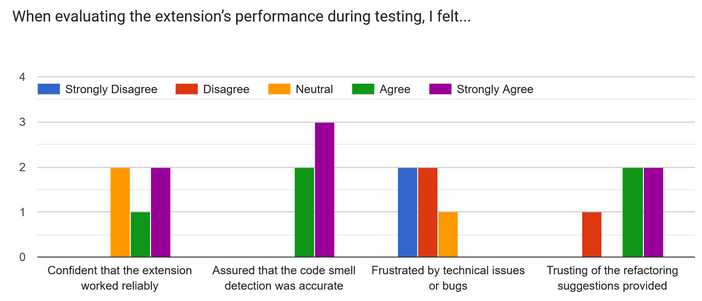
\includegraphics[width=0.7\textwidth]{../Images/usability-satisfaction-graph.png}
  \caption{User Satisfaction Survey Data}
  \label{img:usability-satisfaction}
\end{figure}

\paragraph{Qualitative Results}
Participants found the code smell detection intuitive and accurate,
and they appreciated the preview feature and Accept/Reject buttons.
However, they struggled with sidebar visibility, refactoring speed,
and UI clarity. Hover descriptions were overwhelming, and some
elements (e.g., ``(6/3)'') were unclear. The overall satisfaction ratings can be seen in Figure \ref{img:usability-satisfaction}.

\subsubsection{Discussion}
The usability test revealed that the extension performs well in
detecting code smells and providing refactoring suggestions.
Participants appreciated the energy savings feedback but requested
clearer explanations of how refactoring improves energy efficiency.
The sidebar and refactoring process were identified as major pain
points, requiring immediate attention.\\

The extension met its core functionality objectives but fell short in
UI clarity and performance reliability. Participants expressed
interest in using the extension in the future, provided the
identified issues are addressed. The test highlighted the need for
better onboarding, clearer documentation, and performance
optimizations to enhance user satisfaction and adoption.

\subsubsection{Feedback and Implementation Plan}
The following table summarizes participant feedback and whether the
suggested changes will be implemented:

\begin{table}[H]
  \centering
  \begin{tabular}{>{\raggedright\arraybackslash}p{6cm}p{3.2cm}>{\raggedright\arraybackslash}p{5cm}}
    \toprule \textbf{Feedback} & \textbf{Implementation Decision} &
    \textbf{Reason} \\
    \midrule
    Relocate the sidebar or change its colour for better visibility.
    & Partial & The relocation of the sidebar is not something that
    is in scope during the development period. \\
    Make Accept/Reject buttons more prominent and visually distinct.
    & Yes & High user frustration. \\
    Allow users to customize colours for different types of smells. &
    Yes & Enhances user experience. \\
    Optimize the refactoring process to reduce wait times. & No &
    This is a time intensive ask that is not in scope. \\
    Add progress bars or loading messages to manage user
    expectations. & Yes & Additional messages will be added to the UI.\\
    Provide step-by-step instructions and a tutorial for new users. &
    Yes & This was already planned and will be implemented for revision 1. \\
    Simplify hover descriptions and provide examples or links to
    documentation. & Yes & The hover content will be improved for revision 1. \\
    Explain how refactoring saves energy, possibly with
    visualizations. & Partial & No visualizations will be added, but
    better explanation of smells will be provided. \\
    \bottomrule
  \end{tabular}
  \caption{Participant Feedback and Implementation Decisions}
  \label{tab:participant-feedback}
\end{table}

Based on the feedback summarized in Table \ref{tab:participant-feedback}, we prioritized improvements to the user interface and documentation, focusing on elements that caused the most frustration during testing.\\
\noindent \textbf{Note:} In the Implementation Decision column, ``Partial'' indicates that the issue will not be addressed fully but some changes will be added for the feedback. This means we will implement a limited subset of the suggested improvements that align with our current scope and resource constraints.

\subsection{Performance}

This testing benchmarks the performance of ecooptimizer across
files of varying sizes (250, 1000, and 3000 lines). The data includes
detection times, refactoring times for specific smells, and energy measurement times.
The goal is to identify scalability patterns, performance bottlenecks, and
opportunities for optimization.\\

\textbf{Related Performance Requirement:} PR-1\\

\noindent The test cases for this module can be found
\href{https://github.com/ssm-lab/capstone--source-code-optimizer/blob/new-poc/tests/benchmarking/benchmark.py}{here}\\

This script benchmarks the following components:

\begin{enumerate}
  \item \textbf{Detection/Analyzer Runtime} (via
    \texttt{AnalyzerController.run\_analysis})
  \item \textbf{Refactoring Runtime} (via
    \texttt{RefactorerController.run\_refactorer})
  \item \textbf{Energy Measurement Time} (via
    \texttt{CodeCarbonEnergyMeter.measure\_energy})
\end{enumerate}

For each detected smell (grouped by smell type), refactoring is run
10 times to compute average times.\\

\noindent The following is for your reference: \\

\begin{table}[H]
\centering
\begin{tabular}{|l|l|p{2.5cm}|p{6cm}|}
  \hline
  \textbf{Type of Smell} & \textbf{Code} & \textbf{Smell Name} & \textbf{Brief Explanation} \\
  \hline
  Pylint & R0913 & Long Parameter List & Functions with excessive parameters (beyond configured limit). Complex to refactor as it requires restructuring function signatures and all call sites. \\
  \hline
  Pylint & R6301 & No Self Use & Methods that don't use the instance (self). Requires carefully converting to static methods or class methods. \\
  \hline
  Pylint & R1729 & Use a Generator & List comprehensions that could be generators. Simple transformation but requires ensuring equivalent behavior. \\
  \hline
  Custom & LMC001 & Long Message Chain & Multiple object references chained together (a.b.c.d). Simple to refactor with intermediate variables. \\
  \hline
  Custom & UVA001 & Unused Variable or Attribute & Variables or attributes declared but never used. Easy to remove without complex analysis. \\
  \hline
  Custom & LEC001 & Long Element Chain & Nested dictionary/list access with multiple indexing operations. Simple to refactor with intermediate variables. \\
  \hline
  Custom & LLE001 & Long Lambda Expression & Complex operations in lambda functions. Easy to refactor into named functions. \\
  \hline
  Custom & SCL001 & String Concatenation in Loop & Strings built using += in loops. Simple to refactor to join() or ''.join(). \\
  \hline
  Custom & CRC001 & Cache Repeated Calls & Same function calls made repeatedly with identical parameters. Simple to refactor with caching. \\
  \hline
\end{tabular}
\caption{Code Smells Used in Performance Testing}
\label{tab:code-smells}
\end{table}

\subsubsection{Detection Time vs File Size}
\begin{figure}[H]
  \centering
  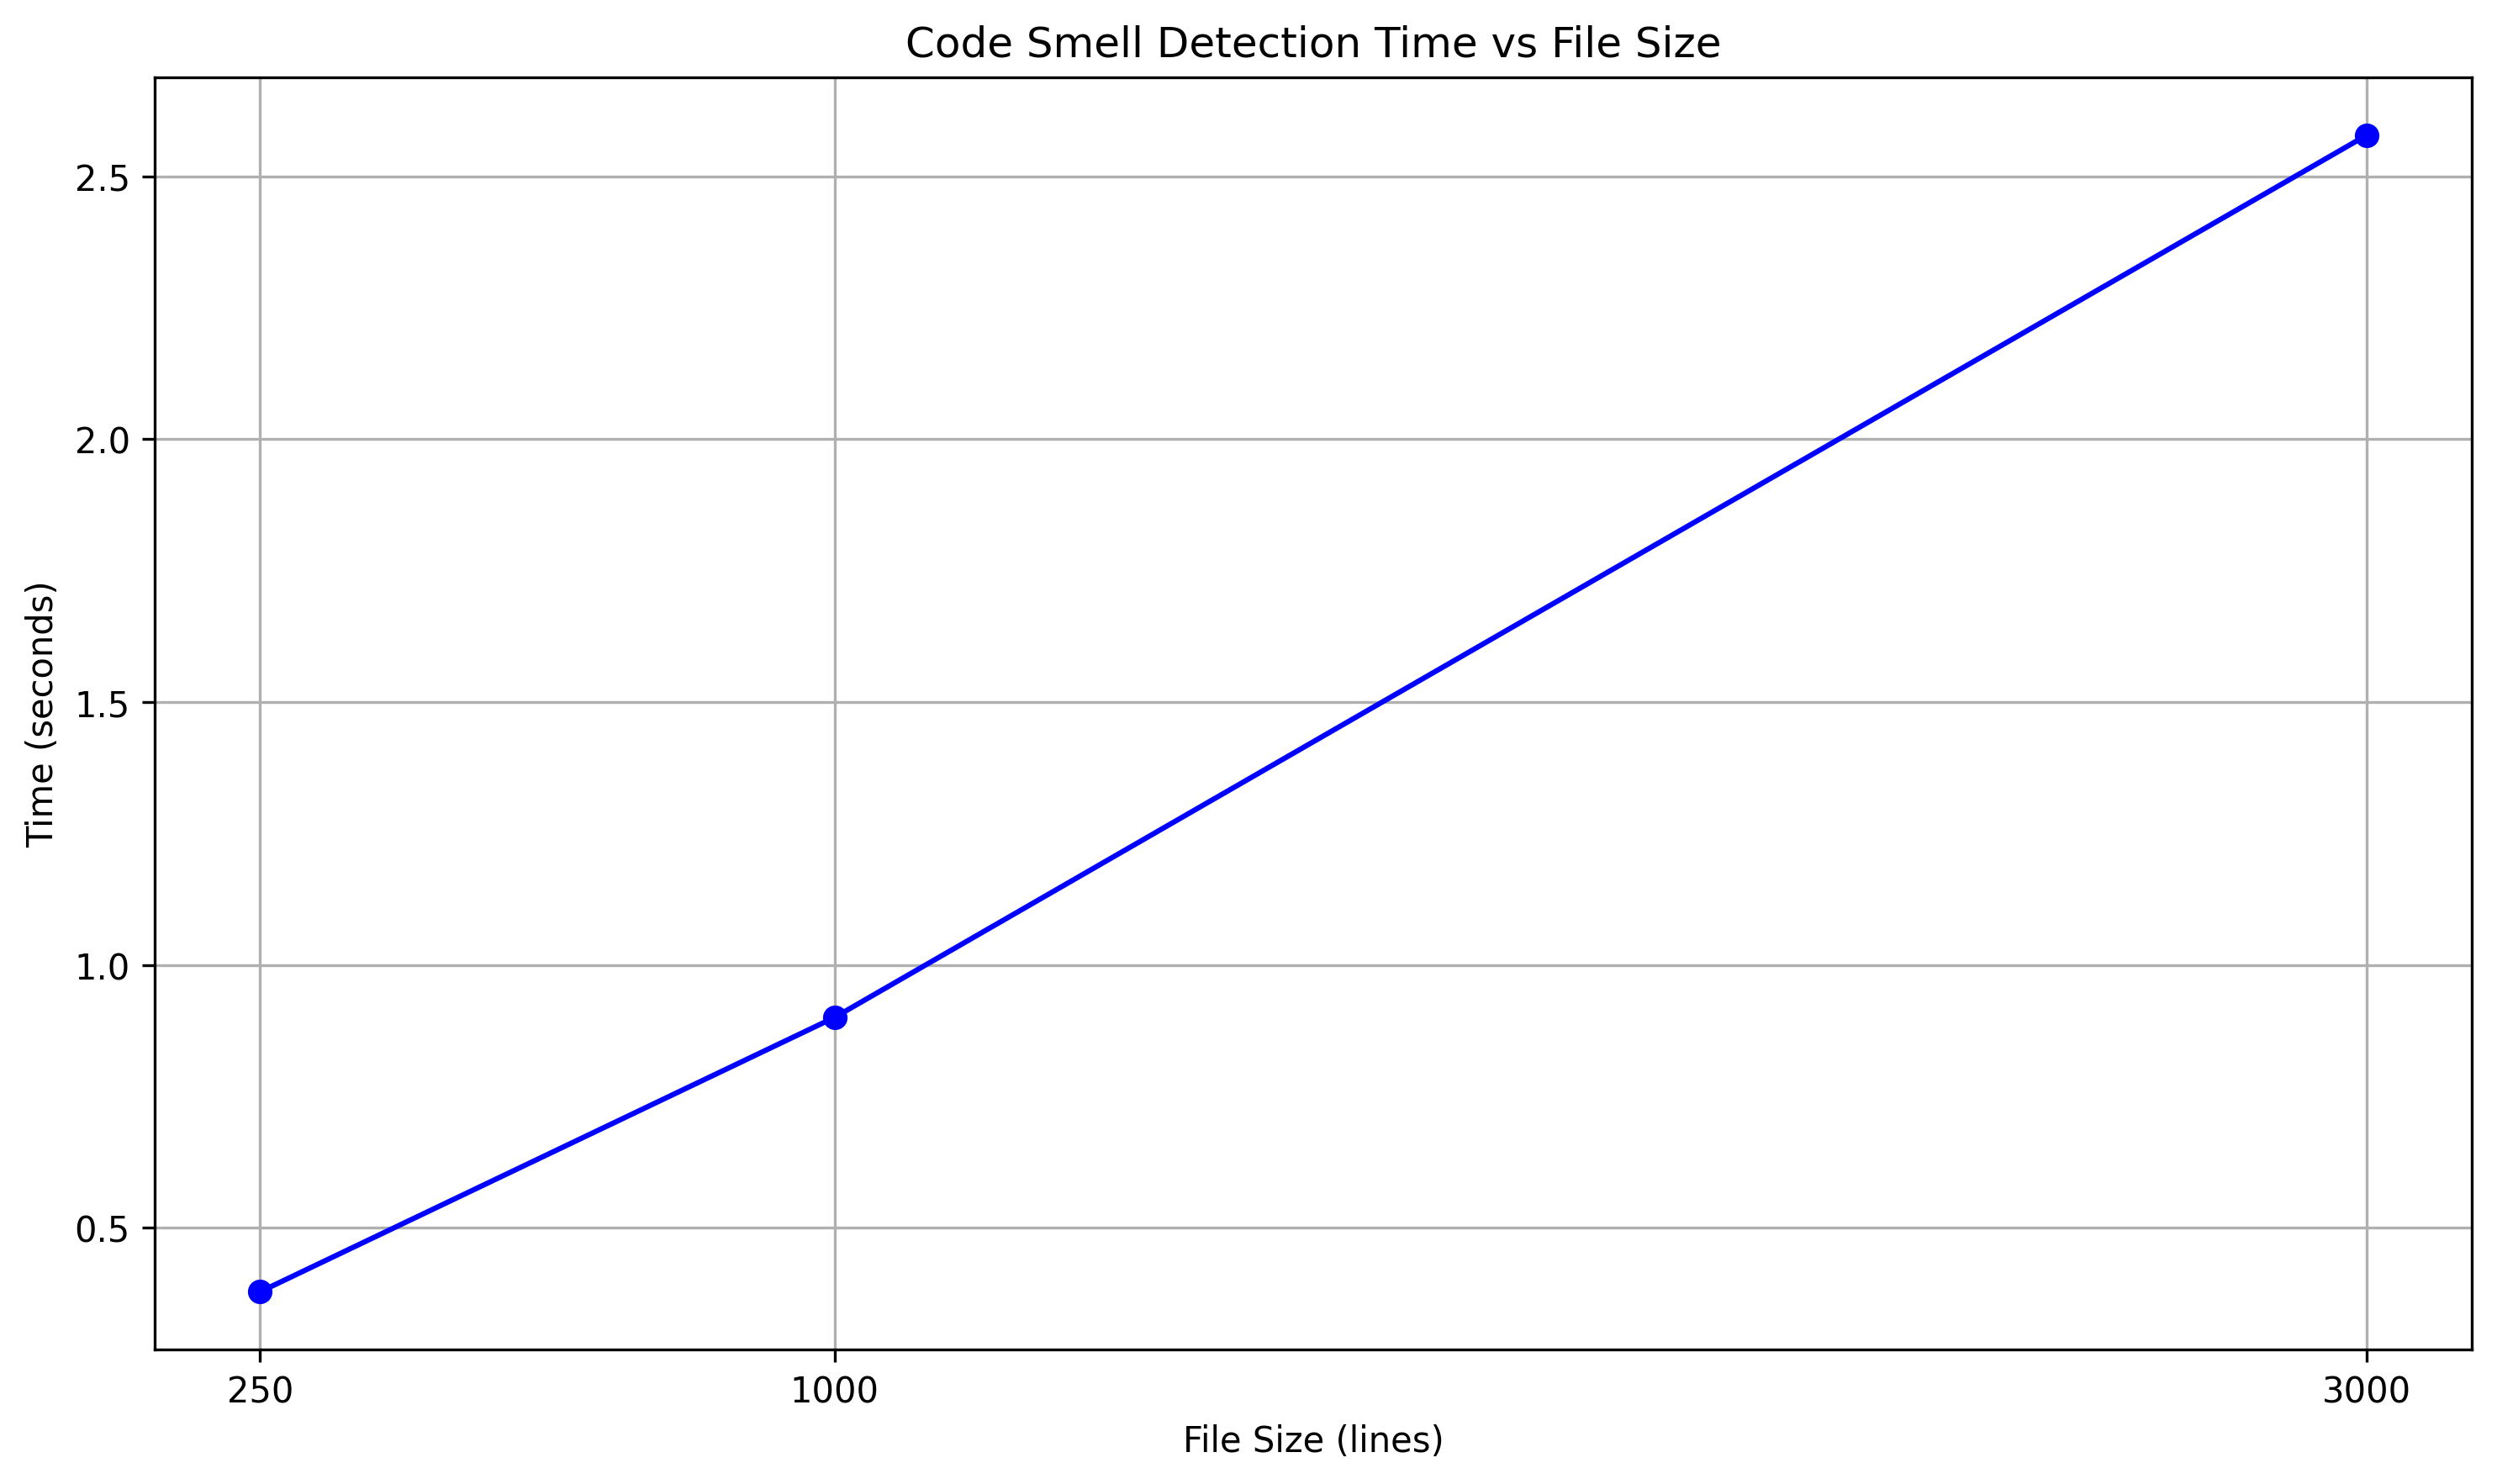
\includegraphics[width=\textwidth]{{../Images/detectionTimeVsFileSize.png}}
  \caption{Detection Time vs File Size}
  \label{fig:detection_time}
\end{figure}

\noindent \textbf{What}: Linear plot showing code smell detection
time growth with file size\\

\noindent \textbf{Why}: Understand scalability of detection mechanism\\

The detection time grows non-linearly with file size, suggesting a
potential \(O(n^2)\) complexity.
For a 250-line file, detection takes 0.38 seconds, while a 1000-line
file takes 0.90 seconds (a 2.4×
increase). At 3000 lines, the detection time jumps to 2.58 seconds (a
2.9× increase from 1000 lines).
This indicates that the detection algorithm scales poorly for larger
files, which could become
problematic for very large codebases. However, the absolute times
remain reasonable, with detection
completing in under 3 seconds even for 3000-line files making this
not a current critical bottleneck, as shown in Figure \ref{fig:detection_time}.

\subsubsection{Refactoring Times by Smell Type (Log Scale)}
\begin{figure}[H]
  \centering
  \includegraphics[width=\textwidth]{../Images/refactoring\_times\_log\_scale.png}
  \caption{Refactoring Times by Smell Type (Log Scale)}
  \label{fig:refactoring_log}
\end{figure}

\noindent \textbf{What}: Logarithmic plot of refactoring times per
smell across file sizes\\

\noindent \textbf{Why}: Identify most expensive refactorings and
scalability patterns\\

The logarithmic plot reveals a clear hierarchy of refactoring costs, as shown in Figure \ref{fig:refactoring_log}.
The most expensive smells are \texttt{R6301} and \texttt{R0913},
which take 6.13 seconds and 5.65 seconds, respectively, for a
3000-line file. These smells show exponential growth, with
\texttt{R6301} increasing by 14.6× from 250 to 3000 lines. In
contrast, low-cost smells like \texttt{LLE001} and \texttt{LMC001}
remain consistently fast (0.03 seconds) across all file sizes. This
suggests that optimizing \texttt{R6301} and \texttt{R0913} should be
a priority, as they dominate the refactoring time for larger files.

\subsubsection{Refactoring Times Heatmap}
\begin{figure}[H]
  \centering
  \includegraphics[width=\textwidth]{../Images/refactoring\_times\_heatmap.png}
  \caption{Refactoring Times Heatmap}
  \label{fig:refactoring_heatmap}
\end{figure}

\noindent \textbf{What}: Color-coded matrix of refactoring times by
smell/file size\\

\noindent \textbf{Why}: Quick visual identification of hot spots\\

The heatmap shown in Figure \ref{fig:refactoring_heatmap} provides a quick visual summary of refactoring times
across smells and file sizes. The darkest cells correspond to
\texttt{R6301} and \texttt{R0913} at 3000 lines, confirming their
status as the most expensive operations. In contrast, \texttt{LLE001}
and \texttt{LMC001} remain light-colored across all sizes, indicating
consistently low costs. The heatmap also highlights the dramatic
variation in refactoring times: at 3000 lines, the fastest smell
(\texttt{LLE001}) is 200× faster than the slowest (\texttt{R6301}).

\subsubsection{Energy Measurement Times Distribution}
\begin{figure}[H]
  \centering
  \includegraphics[width=\textwidth]{../Images/energy\_measurement\_boxplot.png}
  \caption{Energy Measurement Times Distribution}
  \label{fig:energy_boxplot}
\end{figure}

\noindent \textbf{What}: Box plot of energy measurement durations\\

\noindent \textbf{Why}: Verify measurement consistency across operations\\

Energy measurement times are remarkably consistent, ranging from 5.54
to 6.14 seconds across all operations and file sizes, as illustrated in Figure \ref{fig:energy_boxplot}.
The box plot shows no significant variation with file size,
suggesting that energy measurement is operation-specific
rather than dependent on the size of the file. This stability could
indicate that the energy measurement process has a fixed
overhead, which could simplify efforts in the future if we were to
create our own energy measurement module.

\subsubsection{Comparative Refactoring Times per File Size}
\begin{figure}[H]
  \centering
  \includegraphics[width=\textwidth]{../Images/refactoring\_times\_comparison.png}
  \caption{Comparative Refactoring Times per File Size}
  \label{fig:refactoring_comparison}
\end{figure}

\noindent \textbf{What}: Side-by-side bar charts per file size\\

\noindent \textbf{Why}: Direct comparison of refactoring costs at
different scales\\

The side-by-side bar charts in Figure \ref{fig:refactoring_comparison} reveal consistent dominance patterns
across file sizes. \texttt{R6301} and \texttt{R0913} are always the
top two most expensive smells, while \texttt{LLE001} and
\texttt{LMC001} remain the cheapest. Notably, the relative cost
difference between the most and least expensive smells increases with
file size: at 250 lines, the ratio is 100:1, but at 3000 lines, it
grows to 200:1. This suggests that the scalability of refactoring
operations varies significantly by smell type.

\subsubsection{Energy vs Refactoring Time Correlation}

\begin{figure}[H]
  \centering
  \includegraphics[width=\textwidth]{../Images/energy\_refactoring\_correlation.png}
  \caption{Energy vs Refactoring Time Correlation}
  \label{fig:energy_correlation}
\end{figure}

\noindent \textbf{What}: Scatter plot comparing refactoring and
energy measurement times\\

\noindent \textbf{Why}: Identify potential relationships between
effort and energy impact\\

The scatter plot in Figure \ref{fig:energy_correlation} shows no clear correlation between refactoring time
and energy measurement time. Fast refactorings like \texttt{LLE001}
and slow refactorings like \texttt{R6301} both result in energy
measurement times clustered between 5.5 and 6.1 seconds. This makes
perfect sense as the refactoring operations and energy measurement
are disjoint functionalities in the code.

\subsubsection{Key Insights and Recommendations}

\noindent \textbf{Performance Bottlenecks:}
\begin{itemize}
  \item \textbf{Bottleneck Identification:} The smells \texttt{R6301}
    and \texttt{R0913} are the primary bottlenecks, consuming over
    50\% of the total refactoring time for 3000-line files.
    Optimizing these operations should be a top priority.
  \item \textbf{Scalability Concerns:} Both detection and refactoring
    times scale poorly with file size, suggesting \(O(n^2)\)
    complexity. This could become problematic for very large codebases.
  \item \textbf{Low-Hanging Fruit:} Smells like \texttt{LLE001} and
    \texttt{LMC001} are consistently fast to refactor, making them
    ideal candidates for early refactoring efforts.
  \item \textbf{Energy Measurement Stability:} Energy measurement
    times seem consistent across operations and file sizes,
    indicating a fixed overhead. This simplifies efforts to correlate
    refactoring with energy savings.
  \item \textbf{Disproportionate Costs:} The cost difference between
    the most and least expensive smells grows with file size,
    highlighting the need for targeted optimization.
\end{itemize}

\noindent \textbf{Optimization Recommendations:}
The analysis reveals significant scalability challenges for both
detection and refactoring, particularly for smells like
\texttt{R6301} and \texttt{R0913}. While energy measurement times are
stable, their lack of correlation with refactoring time suggests that
additional metrics may be needed to accurately assess energy savings.
Future work should focus on optimizing high-cost operations and
improving the scalability of the detection algorithm.

\subsection{Maintenance and Support}
\begin{enumerate}

  \item \textbf{test-MS-1: Extensibility for New Code Smells and
    Refactorings} \\[2mm]
    To validate the extensibility of our tool, we structured the
    codebase using a modular design, where new code smell detection
    and refactoring functions can
    be easily added as separate components. In simpler terms, each
    refactoring and each custom detection is placed in its own file.
    A code walkthrough confirmed that
    existing modules remain unaffected when adding new detection
    logic. We successfully integrated a sample code smell and its
    corresponding refactoring method with
    minimal changes, ensuring that the new function was accessible
    through the main interface. This demonstrated that our
    architecture supports future expansions without
    disrupting core functionality.
    
    Specifically, we tested the extensibility by implementing the "DUP001" (duplicated list comprehensions) code smell. This smell occurs when the same list comprehension is used multiple times in close proximity, causing unnecessary repeat calculations. The corresponding refactoring method extracts the list comprehension to a variable and reuses the variable. For example:
    
    \begin{verbatim}
    # Original code (with DUP001 smell)
    total_a = sum([x*2 for x in values])
    count_a = len([x*2 for x in values])
    
    # Refactored code
    computed_values = [x*2 for x in values]
    total_a = sum(computed_values)
    count_a = len(computed_values)
    \end{verbatim}
    
    The implementation required:
    1. Adding a new detection module file \texttt{dup001\_detector.py} that scans for repeated list comprehensions
    2. Creating a new refactoring module file \texttt{dup001\_refactor.py} that implements the extraction logic
    3. Registering the new smell and refactoring in the configuration system
    
    The entire process was completed in less than one day, confirming the tool's extensibility target.

  \item \textbf{test-MS-2: Maintainable and Adaptable Codebase} \\[2mm]
    We conducted a static analysis and documentation walkthrough to
    assess the maintainability of our codebase. The code was reviewed
    for modular organization, clear separation
    of concerns, and adherence to coding standards. All modules were
    correctly seperated and organzied. Documentation will be updated
    to include detailed descriptions of functions
    and configuration files, ensuring clarity for future developers.
    Code comments were refined to enhance readability, and function
    naming conventions were standardized for
    consistency. These efforts ensured that the tool remains
    adaptable to new Python versions and evolving best practices.

  \item \textbf{test-MS-3: Easy rollback of updates in case of errors} \\[2mm]
    Once releases are made, each release will be properly tagged and
    versioned to ensure smooth rollbacks through version control.
    This will all be handled with Git. done, but
    this approach guarantees that users will be able to revert to a
    previous stable version if needed, maintaining system integrity
    and minimizing disruptions.
\end{enumerate}

\subsection{Look and Feel}
\begin{enumerate}
  \item \textbf{test-LF-1 Side-by-Side Code Comparison in IDE Plugin} \\[2mm]
    The side-by-side code comparison feature in the IDE plugin was
    tested manually to verify that users can clearly view the
    original and refactored code within the VS Code interface. The
    test followed the procedure outlined in Test-LF-1, which
    specifies that upon initiating a refactoring operation, the
    plugin should display the original and modified versions of the
    code in parallel, allowing users to compare changes effectively.

    The tester performed the test dynamically by opening a sample
    code file within the plugin and applying various refactoring
    operations across all detected code smells. The expected result
    was that the IDE plugin would correctly display the two versions
    side by side, with clear options for users to accept or reject
    each change. The actual result confirmed that the functionality
    operates as expected: refactored code was displayed adjacent to
    the original code, ensuring an intuitive comparison process. The
    tester was also able to interact with the accept/reject buttons,
    verifying their usability and correctness.

    A screenshot of the successful test execution is provided in
    Figure \ref{fig:lf1_test}, illustrating the side-by-side code
    comparison functionality within the IDE plugin.

    \FloatBarrier
    \begin{figure}[h]
      \centering
      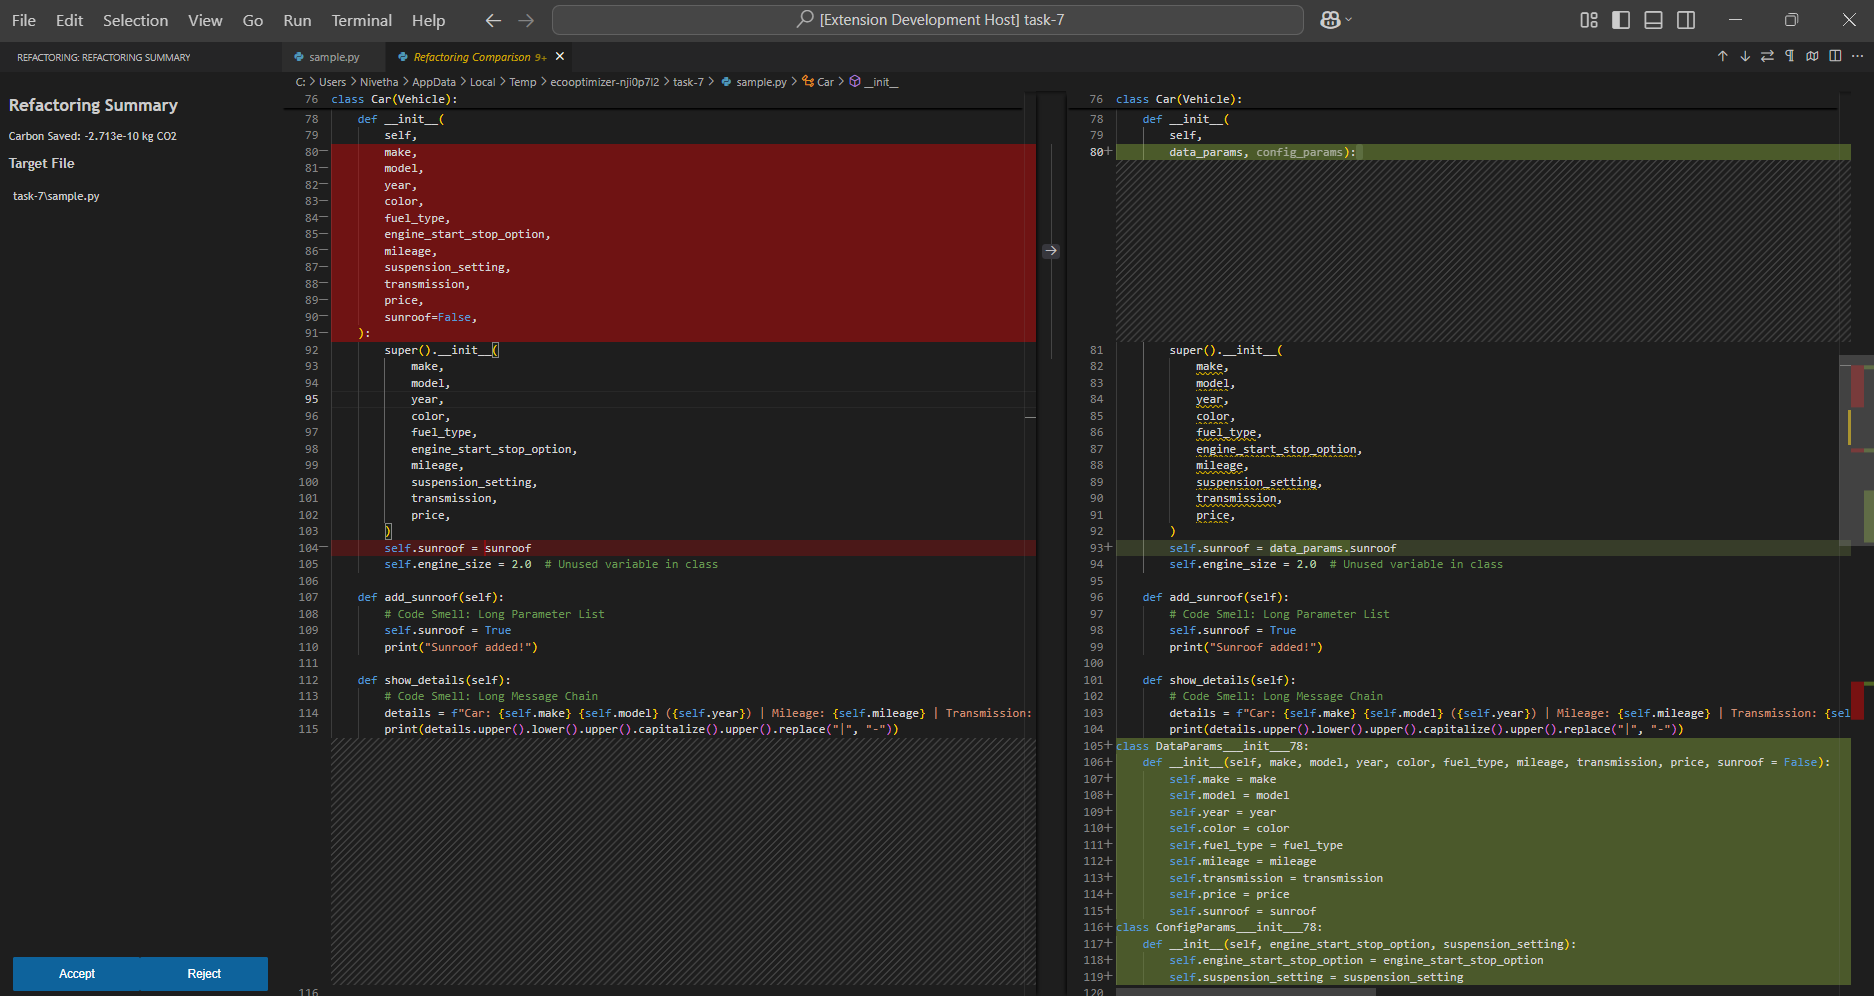
\includegraphics[width=0.8\linewidth]{../Images/test-LF-1-image.png}
      \caption{Side-by-Side Code Comparison in VS Code Plugin}
      \label{fig:lf1_test}
    \end{figure}
    \FloatBarrier

  \item \textbf{test-LF-2 Theme Adaptation in VS Code} \\[2mm]
    The theme adaptation feature in the IDE plugin was tested
    manually to confirm that the plugin correctly adjusts to VS
    Code's light and dark themes without requiring manual
    configuration. The tester performed the test by opening the
    plugin in both themes and switching between them using VS Code's settings.

    The expected result was that the plugin's interface should
    automatically adjust when the theme is changed. The actual result
    confirmed that the plugin seamlessly transitioned between light
    and dark themes while maintaining a consistent interface. The
    images in Figures \ref{fig:lf2_light} and \ref{fig:lf2_dark}
    illustrate the side-by-side refactoring panel in both light mode
    and dark mode.

    \FloatBarrier
    \begin{figure}[h]
      \centering
      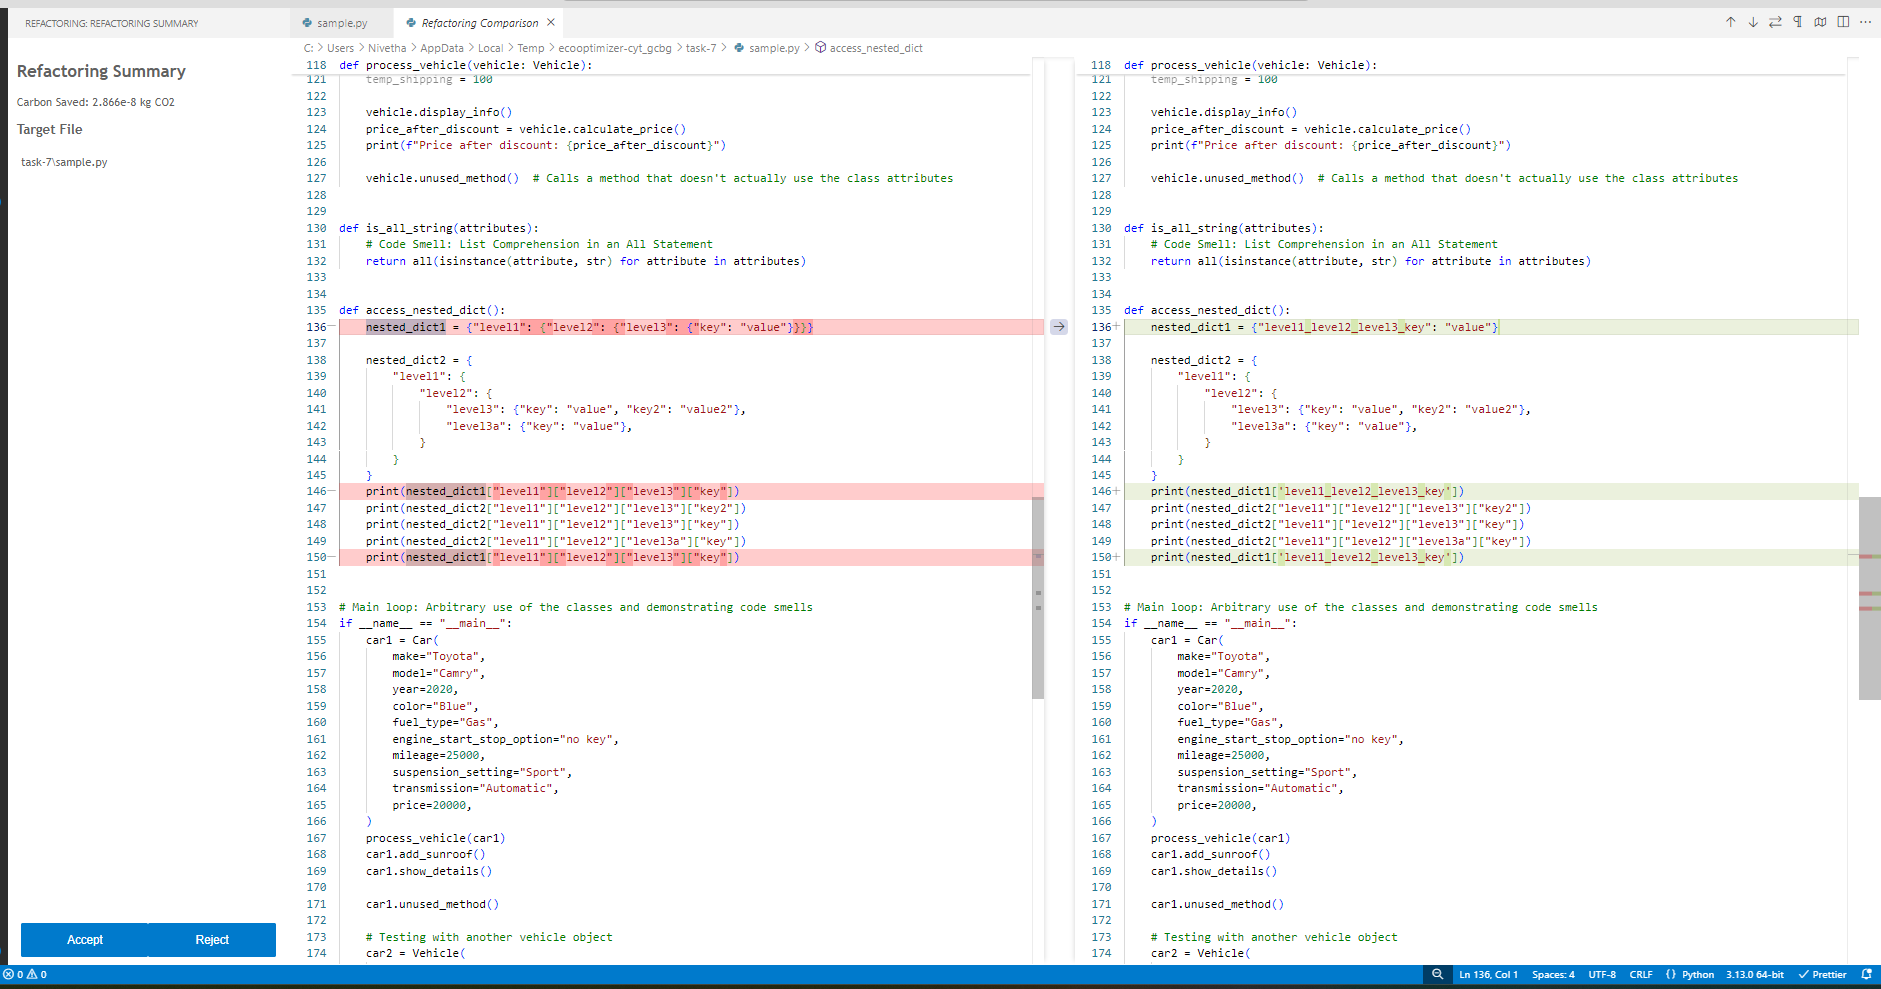
\includegraphics[width=0.8\linewidth]{../Images/test-LF-2-image-light.png}
      \caption{Side-by-Side Refactoring Panel in Light Mode}
      \label{fig:lf2_light}
    \end{figure}
    \FloatBarrier

    \FloatBarrier
    \begin{figure}[h]
      \centering
      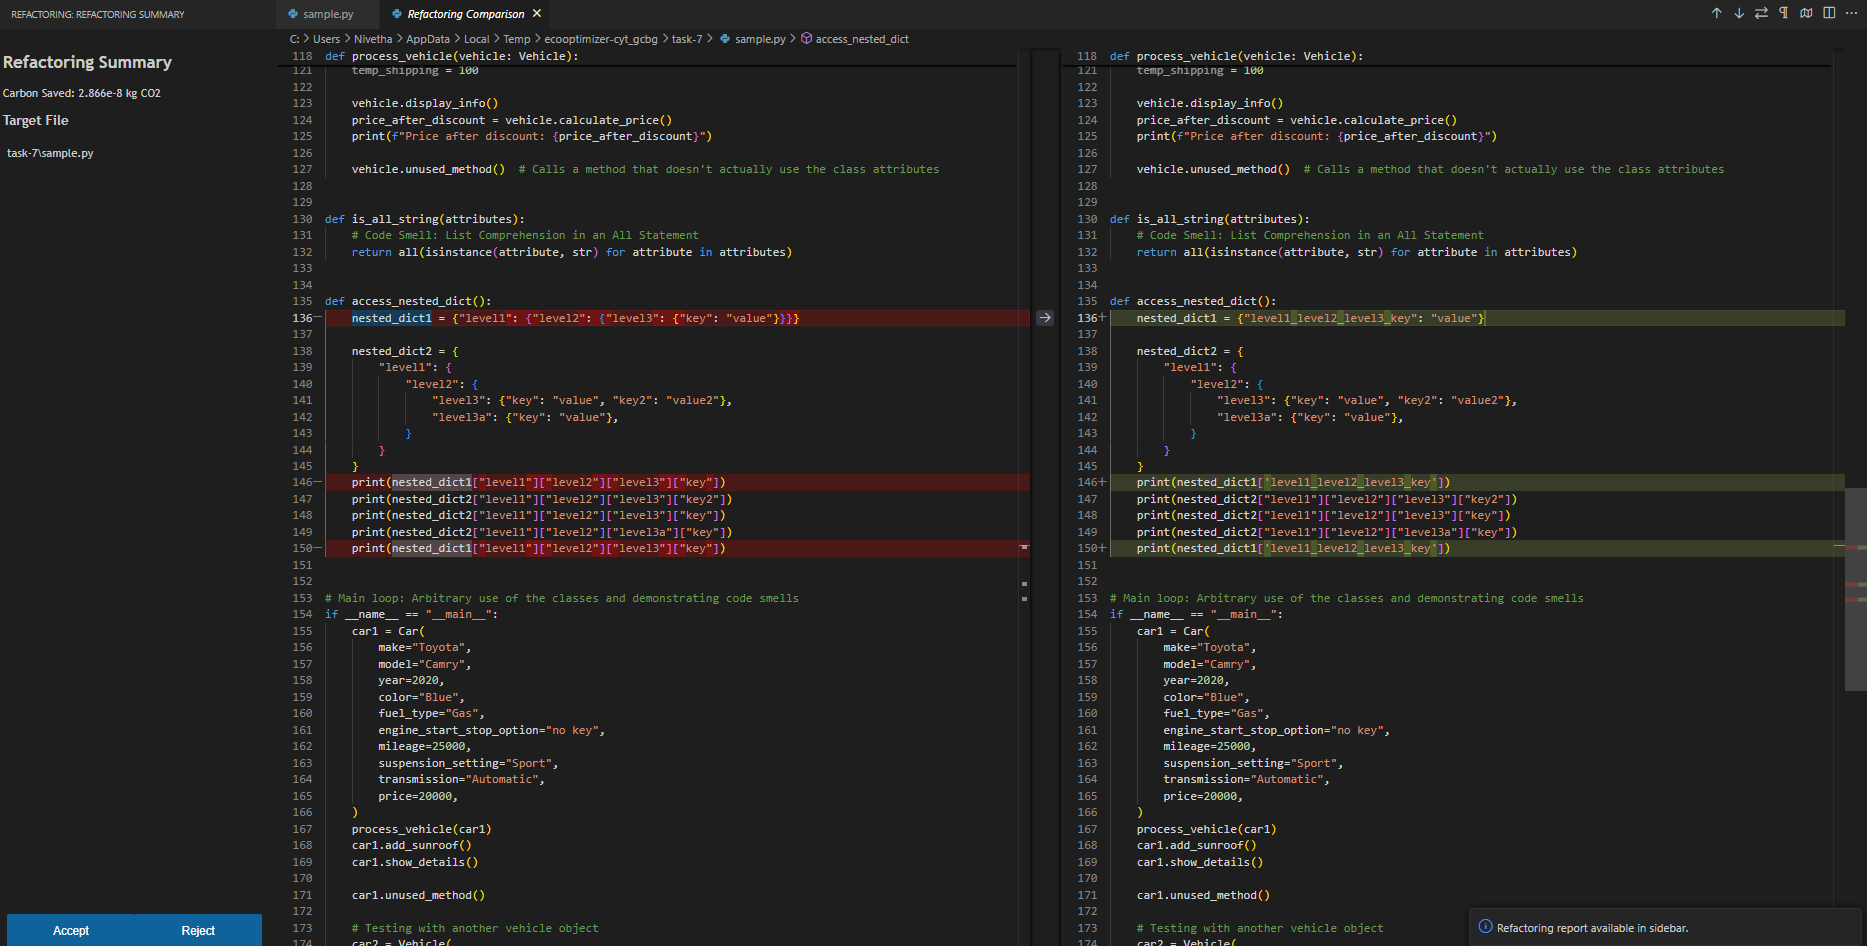
\includegraphics[width=0.8\linewidth]{../Images/test-LF-2-image-dark.png}
      \caption{Side-by-Side Refactoring Panel in Dark Mode}
      \label{fig:lf2_dark}
    \end{figure}
    \FloatBarrier

  \item \textbf{test-LF-3 Design Acceptance} \\[2mm]
    The design acceptance test was conducted as part of the usability
    testing session, where developers and testers interacted with the
    plugin and provided feedback. This test evaluated user
    experience, ease of navigation, and overall satisfaction with the
    plugin's interface.

    The expected result was that users would be able to interact with
    the plugin smoothly and provide structured feedback. The actual
    result confirmed that users were able to navigate and use the
    plugin effectively. The feedback collected during this session
    was used to assess the overall usability of the plugin. More
    details regarding this evaluation can be found in the Usability
    Testing section.

\end{enumerate}

\subsection{Operational \& Environmental}

\textbf{test-OPE-1} will be tested once the extension is officially
launched.\\[2mm]

\noindent
\textbf{test-OPE-2} tests a feature that is yet to be implemented. \\[2mm]

\noindent
\textbf{test-OPE-3} will be tested once the python package is published.

\subsection{Security}

\textbf{test-SRT-1: Audit Logs for Refactoring Processes} \\[2mm]
We conducted a combination of code walkthroughs and static analysis
of logging mechanisms to validate that the tool maintains a secure
log of all refactoring processes, including pattern analysis, energy
analysis, and report generation. The objective was to do so while
covering the logging mechanisms for refactoring events, ensuring that
logs are complete and immutable.\\

\noindent \textbf{Verification Process:} The development team reviewed the codebase to confirm that
each refactoring event (pattern analysis, energy analysis, report
generation) is logged with accurate timestamps and event description.
Missing log entries and/or insufficient details were identified and
added to the logging process.\\

\noindent \textbf{Results:} Through this process, all major refactoring processes were
correctly logged with accurate timestamps. Logs are stored locally on
the user's device, ensuring that unauthorized modifications are
prevented by restricting external access.\\

\noindent \textbf{Conclusion:} The team was able to confirm that the tool maintains a
secure logging system for refactoring processes, with logs being
tamper-resistant due to their local storage on user devices.

\subsection{Compliance}
\begin{enumerate}

  \item \textbf{test-CPL-1: Compliance with PIPEDA and CASL} \\[2mm]
    This process was applied to all processes related to data
    handling and user communication within the local API framework
    with the objective of assesing whether the tool's data handling
    and communication mechanisms align with PIPEDA and CASL
    requirements, ensuring that no personal information is stored,
    all processing is local, and communication practices meet
    regulatory standards.\\
    
    \noindent \textbf{Verification Method:} Through code review, the team confirmed that all data
    processing remains local and does not involve external storage.
    During this time, internal API functionality was also reviewed to
    ensure that user interactions are transient and not logged
    externally. By going through the different workflows, the team
    verified that no personal data collection occurs, eliminating the
    need for explicit consent mechanisms.\\
    
    \noindent \textbf{Compliance Assessment:} As a result of this process, it was concluded that the
    tool does not store any user data. The tool also does not send
    unsolicited communications, aligning with CASL requirements.

  \item \textbf{test-CPL-2: Compliance with ISO 9001 and SSADM
    Standards} \\[2mm]
    This process evaluated development workflows, documentation
    practices, and adherence to structured methodologies with the
    object of assessing whether the tool's quality management and
    software development processes align with ISO 9001 standards for
    quality management and SSADM for structured software development.\\
    
    \noindent \textbf{Evaluation Process:} Through an unbiased approach, the team verified the
    presence of structured documentation, feedback mechanisms, and
    version tracking. It was also confirmed that a combination of
    unit testing, informal testing and iteration processes were
    applied during development. After code review, adherence to
    structured programming and modular design principles was also confirmed.
    
    \noindent \textbf{Development Practices Assessment:} Our goal was to take a third perspective check on
    whether these set of practices were applied to our development
    workflows. Development follows reasonable structured processes
    and also includes formal documentation of testing and quality
    assurance procedures. Version control system is present including
    change tracking and basic project management.

\end{enumerate}

\section{Comparison to Existing Implementation}

Not applicable.

\section{Unit Testing}

The following section outlines the unit tests created for the python
backend modules and the vscode extension.

\newcounter{testcase}
\newcommand{\testcount}{\stepcounter{testcase}\thetestcase}
\renewcommand{\arraystretch}{1.2} % Adjust row height for better readability

\subsection{API Endpoints}

\subsubsection{Smell Detection Endpoint}
The following tests in Table \ref{table:detection_endpoint_tests} verify the functionality of the smell detection API endpoint under various conditions.

\begin{longtable}{c
    >{\raggedright\arraybackslash}p{1.5cm}
    >{\raggedright\arraybackslash}p{4.5cm}
    >{\raggedright\arraybackslash}p{4cm}
  >{\raggedright\arraybackslash}p{3cm} c}
  \toprule
  \textbf{ID} & \textbf{Ref. Req.} & \textbf{Action} &
  \textbf{Expected Result} & \textbf{Actual Result} & \textbf{Result} \\
  \midrule
  \endfirsthead

  \multicolumn{6}{l}{\textit{(Continued from previous page)}} \\
  \toprule
  \textbf{ID} & \textbf{Ref. Req.} & \textbf{Action} &
  \textbf{Expected Result} & \textbf{Actual Result} & \textbf{Result} \\
  \midrule
  \endhead

  \multicolumn{6}{r}{\textit{Continued on next page}} \\
  \endfoot

  \bottomrule
  \caption{Smell Detection Endpoint Test Cases}
  \label{table:detection_endpoint_tests}
  \endlastfoot

  TC\testcount & FR10, OER-IAS1 & User requests to detect smells in a
  valid file. & Status code is 200. Response contains 2 smells. & All
  assertions pass. & \cellcolor{green} Pass \\ \midrule
  TC\testcount & FR10, OER-IAS1 & User requests to detect smells in a
  non-existent file. & Status code is 404. Error message indicates
  file not found. & All assertions pass. & \cellcolor{green} Pass \\ \midrule
  TC\testcount & FR10, OER-IAS1 & Internal server error occurs during
  smell detection. & Status code is 500. Error message indicates
  internal server error. & All assertions pass. & \cellcolor{green} Pass \\
\end{longtable}

\subsubsection{Refactor Endpoint}
Table \ref{table:refactor_endpoint_tests} outlines the test cases for the refactor endpoint, covering both successful operations and error handling scenarios.

\begin{longtable}{c
    >{\raggedright\arraybackslash}p{1.5cm}
    >{\raggedright\arraybackslash}p{4.5cm}
    >{\raggedright\arraybackslash}p{4cm}
  >{\raggedright\arraybackslash}p{3cm} c}
  \toprule
  \textbf{ID} & \textbf{Ref. Req.} & \textbf{Action} &
  \textbf{Expected Result} & \textbf{Actual Result} & \textbf{Result} \\
  \midrule
  \endfirsthead

  \multicolumn{6}{l}{\textit{(Continued from previous page)}} \\
  \toprule
  \textbf{ID} & \textbf{Ref. Req.} & \textbf{Action} &
  \textbf{Expected Result} & \textbf{Actual Result} & \textbf{Result} \\
  \midrule
  \endhead

  \multicolumn{6}{r}{\textit{Continued on next page}} \\
  \endfoot

  \bottomrule
  \caption{Refactor Endpoint Test Cases}
  \label{table:refactor_endpoint_tests}
  \endlastfoot

  TC\testcount & FR10, OER-IAS1 & User requests to refactor a valid
  source directory. & Status code is 200. Response contains
  refactored data and updated smells. & All assertions pass. &
  \cellcolor{green} Pass \\ \midrule
  TC\testcount & FR10, OER-IAS1 & User requests to refactor a
  non-existent source directory. & Status code is 404. Error message
  indicates directory not found. & All assertions pass. &
  \cellcolor{green} Pass \\ \midrule
  TC\testcount & FR10, OER-IAS1 & Energy is not saved after
  refactoring. & Status code is 400. Error message indicates energy
  was not saved. & All assertions pass. & \cellcolor{green} Pass \\ \midrule
  TC\testcount & FR10, OER-IAS1 & Initial energy measurement fails. &
  Status code is 400. Error message indicates initial emissions could
  not be retrieved. & All assertions pass. & \cellcolor{green} Pass \\ \midrule
  TC\testcount & FR10, OER-IAS1 & Final energy measurement fails. &
  Status code is 400. Error message indicates final emissions could
  not be retrieved. & All assertions pass. & \cellcolor{green} Pass \\ \midrule
  TC\testcount & FR10, OER-IAS1 & Unexpected error occurs during
  refactoring. & Status code is 400. Error message contains the
  exception details. & All assertions pass. & \cellcolor{green} Pass \\
  \midrule
  TC\testcount & FR10, OER-IAS1 & User requests to refactor all smells
  of a type successfully. & Status code is 200. Response contains
  refactored data, energy saved, and affected files. & All assertions pass. &
  \cellcolor{green} Pass \\ \midrule
  TC\testcount & FR10, OER-IAS1 & User requests to refactor multiple
  smells of the same type. & Status code is 200. Response contains
  accumulated energy savings from all smells refactored. & All assertions pass. &
  \cellcolor{green} Pass \\ \midrule
  TC\testcount & FR10, OER-IAS1 & Initial energy measurement fails for
  refactor-by-type endpoint. & Status code is 400. Error message indicates
  emissions could not be retrieved. & All assertions pass. &
  \cellcolor{green} Pass \\ \midrule
  TC\testcount & FR10, OER-IAS1 & User requests to refactor all smells
  of a type with nonexistent source directory. & Status code is 404. Error message indicates
  folder not found. & All assertions pass. &
  \cellcolor{green} Pass \\ \midrule
  TC\testcount & FR10, OER-IAS1 & Refactoring error occurs during
  refactor-by-type. & Status code is 500. Error message contains details
  about the refactoring failure. & All assertions pass. &
  \cellcolor{green} Pass \\ \midrule
  TC\testcount & FR10, OER-IAS1 & No energy is saved after refactor-by-type
  operation. & Status code is 400. Error message indicates energy
  was not saved. & All assertions pass. &
  \cellcolor{green} Pass \\ \midrule
  TC\testcount & FR10, OER-IAS1 & Perform refactoring in a new temporary
  directory and validate output. & Temporary directory is created, source is
  copied, smell is refactored, and energy is measured. & All assertions pass. &
  \cellcolor{green} Pass \\ \midrule
  TC\testcount & FR10, OER-IAS1 & Perform refactoring in an existing
  temporary directory. & Uses existing directory, performs refactoring, and
  measures energy without creating new copy. & All assertions pass. &
  \cellcolor{green} Pass \\
\end{longtable}

\subsection{Analyzer Controller Module}
The analyzer controller module was tested extensively to ensure it correctly identifies and processes code smells. Table \ref{table:analyzer_controller_tests} summarizes these test cases.

\begin{longtable}{c
    >{\raggedright\arraybackslash}p{1.5cm}
    >{\raggedright\arraybackslash}p{4.5cm}
    >{\raggedright\arraybackslash}p{4cm}
  >{\raggedright\arraybackslash}p{3cm} c}
  \toprule
  \textbf{ID} & \textbf{Ref. Req.} & \textbf{Action} &
  \textbf{Expected Result} & \textbf{Actual Result} & \textbf{Result} \\
  \midrule
  \endfirsthead

  \multicolumn{6}{l}{\textit{(Continued from previous page)}} \\
  \toprule
  \textbf{ID} & \textbf{Ref. Req.} & \textbf{Action} &
  \textbf{Expected Result} & \textbf{Actual Result} & \textbf{Result} \\
  \midrule
  \endhead

  \multicolumn{6}{r}{\textit{Continued on next page}} \\
  \endfoot

  \bottomrule
  \caption{Analyzer Controller Module Test Cases}
  \label{table:analyzer_controller_tests}
  \endlastfoot

  TC\testcount & FR2, FR5, PR-PAR3 & Test detection of repeated
  function calls in AST-based analysis. & One repeated function call
  should be detected. & All assertions pass. & \cellcolor{green} Pass
  \\ \midrule
  TC\testcount & FR2, FR5, PR-PAR3 & Test detection of repeated
  method calls on the same object instance. & One repeated method
  call should be detected. & All assertions pass. & \cellcolor{green}
  Pass \\ \midrule
  TC\testcount & FR2 & Test that no code smells are detected in a
  clean file. & The system should return an empty list of smells. &
  All assertions pass. & \cellcolor{green} Pass \\ \midrule
  TC\testcount & FR2, PR-PAR2 & Test filtering of smells by analysis
  method. & The function should return only smells matching the
  specified method (AST, Pylint, Astroid). & All assertions pass. &
  \cellcolor{green} Pass \\ \midrule
  TC\testcount & FR2, PR-PAR2 & Test generating custom analysis
  options for AST-based analysis. & The generated options should
  include callable detection functions. & All assertions pass. &
  \cellcolor{green} Pass \\ \midrule
  TC\testcount & FR2, FR5, PR-PAR3 & Test correct logging of detected
  code smells. & Detected smells should be logged with correct
  details. & All assertions pass. & \cellcolor{green} Pass \\ \midrule
  TC\testcount & FR2, FR5 & Test handling of an empty registry when
  filtering smells. & The function should return an empty dictionary.
  & All assertions pass. & \cellcolor{green} Pass \\ \midrule
  TC\testcount & FR2, PR-PAR2 & Test that smells remain unchanged if
  no modifications occur. & The function should not modify existing
  smells if no changes are detected. & All assertions pass. &
  \cellcolor{green} Pass \\
\end{longtable}

\subsection{CodeCarbon Measurement}
The following test cases in Table \ref{table:measurement_tests} were executed to verify the functionality of the CodeCarbon measurement module.

\begin{longtable}{c
    >{\raggedright\arraybackslash}p{1.5cm}
    >{\raggedright\arraybackslash}p{4.5cm}
    >{\raggedright\arraybackslash}p{4cm}
  >{\raggedright\arraybackslash}p{3cm} c}
  \toprule
  \textbf{ID} & \textbf{Ref. Req.} & \textbf{Action} &
  \textbf{Expected Result} & \textbf{Actual Result} & \textbf{Result} \\
  \midrule
  \endfirsthead

  \multicolumn{6}{l}{\textit{(Continued from previous page)}} \\
  \toprule
  \textbf{ID} & \textbf{Ref. Req.} & \textbf{Action} &
  \textbf{Expected Result} & \textbf{Actual Result} & \textbf{Result} \\
  \midrule
  \endhead

  \multicolumn{6}{r}{\textit{Continued on next page}} \\
  \endfoot

  \bottomrule
  \caption{CodeCarbon Measurement Test Cases}
  \label{table:measurement_tests}
  \endlastfoot

  TC\testcount & PR-RFT1, FR6 & Trigger CodeCarbon measurements with
  a valid file path. & CodeCarbon subprocess for the file should be
  invoked at least once. \texttt{EmissionsTracker. start} and
  \texttt{stop} API endpoints should be called. Success message
  ``CodeCarbon measurement completed successfully.'' should be
  logged. & All assertions pass. & \cellcolor{green} Pass \\
  \midrule
  TC\testcount & PR-RFT1 & Trigger CodeCarbon function with a valid
  file path that causes a subprocess failure. & CodeCarbon subprocess
  run should still be invoked. \texttt{EmissionsTracker. start} and
  \texttt{stop} API endpoints should be called. An error message
  ``Error executing file'' should be logged. Returned emissions data
  should be \texttt{None} since the execution failed.& All assertions
  pass. & \cellcolor{green} Pass \\
  \midrule
  TC\testcount & FR5, PR-SCR1 & Results produced by CodeCarbon run
  are at a valid CSV file path and can be read. & Emissions data
  should be read successfully from the CSV file. The function should
  return the last row of emissions data. & All assertions pass. &
  \cellcolor{green} Pass \\
  \midrule
  TC\testcount & PR-RFT1, FR6 & Results produced by CodeCarbon run
  are at a valid CSV file path but the file cannot be read. & An
  error message ``Error reading file'' should be logged. The function
  should return \texttt{None} because the file reading failed. & All
  assertions pass. & \cellcolor{green} Pass \\
  \midrule
  TC\testcount & PR-RFT1, FR5 & Given CSV Path for results produced
  by CodeCarbon does not have a file. & An error message ``File
  \texttt{file path} does not exist.'' should be logged.The function
  should return \texttt{None} since the file does not exist. & All
  assertions pass. & \cellcolor{green} Pass \\
  \midrule
  TC\testcount & PR-RFT1 & Handle unexpected return types from 
  CodeCarbon emissions tracker. & If the tracker returns a non-float
  value (e.g., string), a warning should be logged with message
  ``Unexpected emissions type''. Emissions value should be set to
  \texttt{None}. & All assertions pass. & \cellcolor{green} Pass \\
  \midrule
  TC\testcount & PR-RFT1 & Handle NaN return values from CodeCarbon
  emissions tracker. & If the tracker returns NaN, a warning should
  be logged with message ``Unexpected emissions type''. Emissions
  value should be set to \texttt{None}. & All assertions pass. &
  \cellcolor{green} Pass \\
  \midrule
  TC\testcount & PR-RFT1 & Handle missing emissions file after
  measurement. & If the emissions CSV file does not exist after 
  tracking, an error message ``Emissions file missing - measurement
  failed'' should be logged. Emissions\_data should be \texttt{None}. &
  All assertions pass. & \cellcolor{green} Pass \\
\end{longtable}

\subsection{Smell Analyzers}

\subsubsection{String Concatenation in Loop}

\begin{longtable}{c
    >{\raggedright\arraybackslash}p{1.5cm}
    >{\raggedright\arraybackslash}p{4.5cm}
    >{\raggedright\arraybackslash}p{4cm}
  >{\raggedright\arraybackslash}p{3cm} c}
  \toprule
  \textbf{ID} & \textbf{Ref. Req.} & \textbf{Action} &
  \textbf{Expected Result} & \textbf{Actual Result} & \textbf{Result} \\
  \midrule
  \endfirsthead

  \multicolumn{6}{l}{\textit{(Continued from previous page)}} \\
  \toprule
  \textbf{ID} & \textbf{Ref. Req.} & \textbf{Action} &
  \textbf{Expected Result} & \textbf{Actual Result} & \textbf{Result} \\
  \midrule
  \endhead

  \multicolumn{6}{r}{\textit{Continued on next page}} \\
  \endfoot

  \bottomrule
  \caption{String Concatenation in Loop Detection Test Cases}
  \label{table:string_concat_detection_tests}
  \endlastfoot

  TC\testcount & FR2 & Detects \texttt{+=} string concatenation
  inside a \texttt{for} loop. & One smell detected with target
  \texttt{result} and line 4. & All assertions pass. & \cellcolor{green} Pass \\
  \midrule
  TC\testcount & FR2 & Detects \texttt{<var = var + ...>} string
  concatenation inside a loop. & One smell detected with target
  \texttt{result} and line 4. & All assertions pass. & \cellcolor{green} Pass \\
  \midrule
  TC\testcount & FR2 & Detects \texttt{+=} string concatenation
  inside a \texttt{while} loop. & One smell detected with target
  \texttt{result} and line 4. & All assertions pass. & \cellcolor{green} Pass \\
  \midrule
  TC\testcount & FR2 & Detects \texttt{+=} modifying a list item
  inside a loop. & One smell detected with target
  \lstinline|self.text[0]| and line 6. & All assertions pass. &
  \cellcolor{green} Pass \\
  \midrule
  TC\testcount & FR2 & Detects \texttt{+=} modifying an object
  attribute inside a loop. & One smell detected with target
  \lstinline|self.text| and line 6. & All assertions pass. &
  \cellcolor{green} Pass \\
  \midrule
  TC\testcount & FR2 & Detects \texttt{+=} modifying a dictionary
  value inside a loop. & One smell detected with target
  \texttt{data['key']} and line 4. & All assertions pass. &
  \cellcolor{green} Pass \\
  \midrule
  TC\testcount & FR2 & Detects multiple separate string
  concatenations in a loop. & Two smells detected with targets
  \texttt{result} and \texttt{logs[0]} on line 5. & All assertions
  pass. & \cellcolor{green} Pass \\
  \midrule
  TC\testcount & FR2 & Detects string concatenations with
  re-assignments inside the loop. & One smell detected with target
  \texttt{result} and line 4. & All assertions pass. & \cellcolor{green} Pass \\
  \midrule
  TC\testcount & FR2 & Detects concatenation inside nested loops. &
  One smell detected with target \texttt{result} and line 5. & All
  assertions pass. & \cellcolor{green} Pass \\
  \midrule
  TC\testcount & FR2 & Detects multi-level concatenations belonging
  to the same smell. & One smell detected with target \texttt{result}
  and two occurrences on lines 4 and 5. & All assertions pass. &
  \cellcolor{green} Pass \\
  \midrule
  TC\testcount & FR2 & Detects \texttt{+=} inside an \texttt{if-else}
  condition within a loop. & One smell detected with target
  \texttt{result} and two occurrences on line 4. & All assertions
  pass. & \cellcolor{green} Pass \\
  \midrule
  TC\testcount & FR2 & Detects \texttt{+=} using f-strings inside a
  loop. & One smell detected with target \texttt{result} and line 4.
  & All assertions pass. & \cellcolor{green} Pass \\
  \midrule
  TC\testcount & FR2 & Detects \texttt{+=} using \texttt{\%}
  formatting inside a loop. & One smell detected with target
  \texttt{result} and line 4. & All assertions pass. & \cellcolor{green} Pass \\
  \midrule
  TC\testcount & FR2 & Detects \texttt{+=} using \texttt{.format()}
  inside a loop. & One smell detected with target \texttt{result} and
  line 4. & All assertions pass. & \cellcolor{green} Pass \\
  \midrule
  TC\testcount & FR2 & Ensures accessing the concatenation variable
  inside the loop is NOT flagged. & No smells detected. & All
  assertions pass. & \cellcolor{green} Pass \\
  \midrule
  TC\testcount & FR2 & Ensures regular string assignments are NOT
  flagged. & No smells detected. & All assertions pass. &
  \cellcolor{green} Pass \\
  \midrule
  TC\testcount & FR2 & Ensures number operations with \texttt{+=} are
  NOT flagged. & No smells detected. & All assertions pass. &
  \cellcolor{green} Pass \\
  \midrule
  TC\testcount & FR2 & Ensures string concatenation OUTSIDE a loop is
  NOT flagged. & No smells detected. & All assertions pass. &
  \cellcolor{green} Pass \\
  \midrule
  TC\testcount & FR2 & Detects a variable concatenated multiple times
  in the same loop iteration. & One smell detected with target
  \texttt{result} and two occurrences on line 4. & All assertions
  pass. & \cellcolor{green} Pass \\
  \midrule
  TC\testcount & FR2 & Detects concatenation where both prefix and
  suffix are added. & One smell detected with target \texttt{result}
  and line 4. & All assertions pass. & \cellcolor{green} Pass \\
  \midrule
  TC\testcount & FR2 & Detects \texttt{+=} where new values are
  inserted at the beginning instead of the end. & One smell detected
  with target \texttt{result} and line 4. & All assertions pass. &
  \cellcolor{green} Pass \\
  \midrule
  TC\testcount & FR2 & Ignores potential smells where type cannot be
  confirmed as a string. & No smells detected. & All assertions pass.
  & \cellcolor{green} Pass \\
  \midrule
  TC\testcount & FR2 & Detects string concatenation where type is
  inferred from function type hints. & One smell detected with target
  \texttt{result} and line 4. & All assertions pass. & \cellcolor{green} Pass \\
  \midrule
  TC\testcount & FR2 & Detects string concatenation where type is
  inferred from variable type hints. & One smell detected with target
  \texttt{result} and line 4. & All assertions pass. & \cellcolor{green} Pass \\
  \midrule
  TC\testcount & FR2 & Detects string concatenation where type is
  inferred from class attributes. & One smell detected with target
  \texttt{result} and line 9. & All assertions pass. & \cellcolor{green} Pass \\
  \midrule
  TC\testcount & FR2 & Detects string concatenation where type is
  inferred from the initial value assigned. & One smell detected with
  target \texttt{result} and line 4. & All assertions pass. &
  \cellcolor{green} Pass \\
\end{longtable}

\subsubsection{Long Element Chain Detector Module}

\begin{longtable}{c
    >{\raggedright\arraybackslash}p{1.5cm}
    >{\raggedright\arraybackslash}p{4.5cm}
    >{\raggedright\arraybackslash}p{4cm}
  >{\raggedright\arraybackslash}p{3cm} c}
  \toprule
  \textbf{ID} & \textbf{Ref. Req.} & \textbf{Action} &
  \textbf{Expected Result} & \textbf{Actual Result} & \textbf{Result} \\
  \midrule
  \endfirsthead

  \multicolumn{6}{l}{\textit{(Continued from previous page)}} \\
  \toprule
  \textbf{ID} & \textbf{Ref. Req.} & \textbf{Action} &
  \textbf{Expected Result} & \textbf{Actual Result} & \textbf{Result} \\
  \midrule
  \endhead

  \multicolumn{6}{r}{\textit{Continued on next page}} \\
  \endfoot

  \bottomrule
  \caption{Long Element Chain Detector Module Test Cases}
  \label{table:lec_tests}
  \endlastfoot

  TC\testcount & FR2 & Test with code that has no chains. & No chains
  should be detected. & All assertions pass. & \cellcolor{green} Pass
  \\ \midrule
  TC\testcount & FR2 & Test with chains shorter than threshold. & No
  chains should be detected for threshold of 5. & All assertions
  pass. & \cellcolor{green} Pass \\ \midrule
  TC\testcount & FR2  & Test with chains exactly at threshold. & One
  chain should be detected at line 3. & All assertions pass. &
  \cellcolor{green} Pass \\ \midrule
  TC\testcount & FR2 & Test with chains longer than threshold. & One
  chain should be detected with message ``Dictionary chain too long
  (4/3)''. & All assertions pass. & \cellcolor{green} Pass \\ \midrule
  TC\testcount & FR2 & Test with multiple chains in the same file. &
  Two chains should be detected at different lines. & All assertions
  pass. & \cellcolor{green} Pass \\ \midrule
  TC\testcount & FR2 & Test chains inside nested functions and
  classes. & Two chains should be detected, one inside a function,
  one inside a class. & All assertions pass. & \cellcolor{green} Pass
  \\ \midrule
  TC\testcount & FR2 & Test that chains on the same line are reported
  only once. & One chain should be detected at line 4. & All
  assertions pass. & \cellcolor{green} Pass \\ \midrule
  TC\testcount & FR2 & Test chains with different variable types. &
  Two chains should be detected, one in a list and one in a tuple. &
  All assertions pass. & \cellcolor{green} Pass \\ \midrule
  TC\testcount & FR2 & Test with a custom threshold value. & No
  chains detected with threshold 4. One chain detected with threshold
  2. & All assertions pass. & \cellcolor{green} Pass \\ \midrule
  TC\testcount & FR2 & Test the structure of the returned LECSmell
  object. & Object should have correct type, path, module, symbol,
  and occurrence details. & All assertions pass. & \cellcolor{green}
  Pass \\ \midrule
  TC\testcount & FR2 & Test chains within complex expressions. &
  Three chains should be detected in different contexts. & All
  assertions pass. & \cellcolor{green} Pass \\ \midrule
  TC\testcount & FR2 & Test with an empty file. & No chains should be
  detected. & All assertions pass. & \cellcolor{green} Pass \\ \midrule
  TC\testcount & FR2 & Test with threshold of 1 (every subscript
  reported). & One chain should be detected with message ``Dictionary
  chain too long (5/5)''. & All assertions pass. & \cellcolor{green} Pass \\
\end{longtable}

\subsubsection{Repeated Calls Detection Module}

\begin{longtable}{c
    >{\raggedright\arraybackslash}p{1.5cm}
    >{\raggedright\arraybackslash}p{4.5cm}
    >{\raggedright\arraybackslash}p{4cm}
  >{\raggedright\arraybackslash}p{3cm} c}
  \toprule
  \textbf{ID} & \textbf{Ref. Req.} & \textbf{Action} &
  \textbf{Expected Result} & \textbf{Actual Result} & \textbf{Result} \\
  \midrule
  \endfirsthead

  \multicolumn{6}{l}{\textit{(Continued from previous page)}} \\
  \toprule
  \textbf{ID} & \textbf{Ref. Req.} & \textbf{Action} &
  \textbf{Expected Result} & \textbf{Actual Result} & \textbf{Result} \\
  \midrule
  \endhead

  \multicolumn{6}{r}{\textit{Continued on next page}} \\
  \endfoot

  \bottomrule
  \caption{Repeated Calls Detection Module Test Cases}
  \label{table:crc_tests}
  \endlastfoot

  TC\testcount & FR2, PR-PAR2 & Test detection of repeated function
  calls within the same scope. & One repeated call detected with two
  occurrences. & All assertions pass. & \cellcolor{green} Pass \\ \midrule
  TC\testcount & FR2, PR-PAR2 & Test detection of repeated method
  calls on the same object instance. & One repeated method call
  detected with two occurrences. & All assertions pass. &
  \cellcolor{green} Pass \\ \midrule
  TC\testcount & FR2 & Test that function calls with different
  arguments are not flagged. & No repeated calls should be detected.
  & All assertions pass. & \cellcolor{green} Pass \\ \midrule
  TC\testcount & FR2 & Test that function calls on modified objects
  are not flagged. & No repeated calls should be detected due to
  object state change. & All assertions pass. & \cellcolor{green}
  Pass \\ \midrule
  TC\testcount & FR2, PR-PAR3 & Test detection of repeated external
  function calls. & One repeated function call detected with two
  occurrences. & All assertions pass. & \cellcolor{green} Pass \\ \midrule
  TC\testcount & FR2, PR-PAR3 & Test detection of repeated calls to
  expensive built-in functions. & One repeated function call detected
  with two occurrences. & All assertions pass. & \cellcolor{green}
  Pass \\ \midrule
  TC\testcount & FR2, PR-PAR3 & Test that built-in functions with
  primitive arguments are not flagged. & No repeated calls should be
  detected. & All assertions pass. & \cellcolor{green} Pass \\ \midrule
  TC\testcount & FR2 & Test that method calls on different object
  instances are not flagged. & No repeated calls should be detected.
  & All assertions pass. & \cellcolor{green} Pass \\
\end{longtable}

\subsubsection{Long Lambda Element Detection Module}

\begin{longtable}{c
    >{\raggedright\arraybackslash}p{1.5cm}
    >{\raggedright\arraybackslash}p{4.5cm}
    >{\raggedright\arraybackslash}p{4cm}
  >{\raggedright\arraybackslash}p{3cm} c}
  \toprule
  \textbf{ID} & \textbf{Ref. Req.} & \textbf{Action} &
  \textbf{Expected Result} & \textbf{Actual Result} & \textbf{Result} \\
  \midrule
  \endfirsthead

  \multicolumn{6}{l}{\textit{(Continued from previous page)}} \\
  \toprule
  \textbf{ID} & \textbf{Ref. Req.} & \textbf{Action} &
  \textbf{Expected Result} & \textbf{Actual Result} & \textbf{Result} \\
  \midrule
  \endhead

  \multicolumn{6}{r}{\textit{Continued on next page}} \\
  \endfoot

  \bottomrule
  \caption{Long Lambda Element Detector Module Test Cases}
  \label{table:lle_tests}
  \endlastfoot

  TC\testcount & FR2 & Test code with no lambdas. & No smells should
  be detected. & All assertions pass. & \cellcolor{green} Pass \\ \midrule
  TC\testcount & FR2 & Test short single lambda (under thresholds). &
  No smells should be detected. & All assertions pass. &
  \cellcolor{green} Pass \\ \midrule
  TC\testcount & FR2 & Test lambda exceeding expression count
  threshold. & One smell should be detected. & All assertions pass. &
  \cellcolor{green} Pass \\ \midrule
  TC\testcount & FR2 & Test lambda exceeding character length
  threshold (100). & One smell should be detected. & All assertions
  pass. & \cellcolor{green} Pass \\ \midrule
  TC\testcount & FR2 & Test lambda exceeding both expression and
  length thresholds. & At least one smell should be detected. & All
  assertions pass. & \cellcolor{green} Pass \\ \midrule
  TC\testcount & FR2 & Test nested lambdas. & Two smells should be
  detected. & All assertions pass. & \cellcolor{green} Pass \\ \midrule
  TC\testcount & FR2 & Test inline lambdas passed to functions. & Two
  smells should be detected. & All assertions pass. &
  \cellcolor{green} Pass \\ \midrule
  TC\testcount & FR2 & Test trivial lambda with no body. & No smells
  should be detected. & All assertions pass. & \cellcolor{green} Pass \\
\end{longtable}

\subsubsection{Long Message Chain Detector Module}

\begin{longtable}{c
    >{\raggedright\arraybackslash}p{1.5cm}
    >{\raggedright\arraybackslash}p{4.5cm}
    >{\raggedright\arraybackslash}p{4cm}
  >{\raggedright\arraybackslash}p{3cm} c}
  \toprule
  \textbf{ID} & \textbf{Ref. Req.} & \textbf{Action} &
  \textbf{Expected Result} & \textbf{Actual Result} & \textbf{Result} \\
  \midrule
  \endfirsthead

  \multicolumn{6}{l}{\textit{(Continued from previous page)}} \\
  \toprule
  \textbf{ID} & \textbf{Ref. Req.} & \textbf{Action} &
  \textbf{Expected Result} & \textbf{Actual Result} & \textbf{Result} \\
  \midrule
  \endhead

  \multicolumn{6}{r}{\textit{Continued on next page}} \\
  \endfoot

  \bottomrule
  \caption{Long Message Chain Detector Module Test Cases}
  \label{table:lmc_tests}
  \endlastfoot

  TC\testcount & FR2 & Test chain with exactly five method calls. &
  One smell should be detected. & All assertions pass. &
  \cellcolor{green} Pass \\ \midrule
  TC\testcount & FR2 & Test chain with six method calls. & One smell
  should be detected. & All assertions pass. & \cellcolor{green} Pass
  \\ \midrule
  TC\testcount & FR2 & Test chain with four method calls. & No smells
  should be detected. & All assertions pass. & \cellcolor{green} Pass
  \\ \midrule
  TC\testcount & FR2 & Test chain with both attribute and method
  calls. & One smell should be detected. & All assertions pass. &
  \cellcolor{green} Pass \\ \midrule
  TC\testcount & FR2 & Test chain inside a loop. & One smell should
  be detected. & All assertions pass. & \cellcolor{green} Pass \\ \midrule
  TC\testcount & FR2 & Test multiple chains on the same line. & One
  smell should be detected. & All assertions pass. &
  \cellcolor{green} Pass \\ \midrule
  TC\testcount & FR2 & Test separate statements with fewer calls. &
  No smells should be detected. & All assertions pass. &
  \cellcolor{green} Pass \\ \midrule
  TC\testcount & FR2 & Test short chain in a comprehension. & No
  smells should be detected. & All assertions pass. &
  \cellcolor{green} Pass \\ \midrule
  TC\testcount & FR2 & Test long chain in a comprehension. & One
  smell should be detected. & All assertions pass. &
  \cellcolor{green} Pass \\ \midrule
  TC\testcount & FR2 & Test five separate long chains in one
  function. & Five smells should be detected. & All assertions pass.
  & \cellcolor{green} Pass \\ \midrule
  TC\testcount & FR2 & Test chain with attribute and index lookups
  (no calls). & No smells should be detected. & All assertions pass.
  & \cellcolor{green} Pass \\ \midrule
  TC\testcount & FR2 & Test chain with slicing. & One smell should be
  detected. & All assertions pass. & \cellcolor{green} Pass \\ \midrule
  TC\testcount & FR2 & Test multiline chain. & One smell should be
  detected. & All assertions pass. & \cellcolor{green} Pass \\ \midrule
  TC\testcount & FR2 & Test chain inside a lambda. & One smell should
  be detected. & All assertions pass. & \cellcolor{green} Pass \\ \midrule
  TC\testcount & FR2 & Test chain with mixed return types. & One
  smell should be detected. & All assertions pass. &
  \cellcolor{green} Pass \\ \midrule
  TC\testcount & FR2 & Test multiple short chains on the same line. &
  No smells should be detected. & All assertions pass. &
  \cellcolor{green} Pass \\ \midrule
  TC\testcount & FR2 & Test chain inside a conditional (ternary). &
  No smells should be detected. & All assertions pass. &
  \cellcolor{green} Pass \\
\end{longtable}

\subsection{Refactorer Controller Module}

\begin{longtable}{c
    >{\raggedright\arraybackslash}p{1.5cm}
    >{\raggedright\arraybackslash}p{4.5cm}
    >{\raggedright\arraybackslash}p{4cm}
  >{\raggedright\arraybackslash}p{3cm} c}
  \toprule
  \textbf{ID} & \textbf{Ref. Req.} & \textbf{Action} &
  \textbf{Expected Result} & \textbf{Actual Result} & \textbf{Result} \\
  \midrule
  \endfirsthead

  \multicolumn{6}{l}{\textit{(Continued from previous page)}} \\
  \toprule
  \textbf{ID} & \textbf{Ref. Req.} & \textbf{Action} &
  \textbf{Expected Result} & \textbf{Actual Result} & \textbf{Result} \\
  \midrule
  \endhead

  \multicolumn{6}{r}{\textit{Continued on next page}} \\
  \endfoot

  \bottomrule
  \caption{Refactorer Controller Module Test Cases}
  \label{table:refactorer_controller_tests}
  \endlastfoot

  TC\testcount & FR5 & User requests to refactor a smell. & Correct
  smell is identified. Logger logs ``Running refactoring for
  long-element-chain using TestRefactorer.'' Correct refactorer is
  called once with correct arguments. Output path is
  \texttt{test\_path.LEC001\_1.py}. & All assertions pass. &
  \cellcolor{green} Pass \\ \midrule
  TC\testcount & UHR-UPLD1 & System handles missing refactorer. &
  Raises \texttt{NotImplementedError} with message ``No refactorer
  implemented for smell: long-element-chain.'' Logger logs error. &
  All assertions pass. & \cellcolor{green} Pass \\ \midrule
  TC\testcount & FR5 & Multiple refactorer calls are handled
  correctly. & Correct smell counter incremented. Refactorer is
  called twice. First output: \texttt{test\_path.LEC001\_1.py}.
  Second output: \texttt{test\_path.LEC001\_2.py}. & All assertions
  pass. & \cellcolor{green} Pass \\ \midrule
  TC\testcount & FR5 & Refactorer runs with overwrite set to False. &
  Refactorer is called once. Overwrite argument is set to False. &
  All assertions pass. & \cellcolor{green} Pass \\ \midrule
  TC\testcount & PR-RFT 1, FR5 & System handles empty modified files
  correctly. & Modified files list remains empty (\texttt{[]} in
  output). & All assertions pass. & \cellcolor{green} Pass \\
\end{longtable}

\subsection{Smell Refactorers}

\subsubsection{String Concatenation in Loop}

\begin{longtable}{c
    >{\raggedright\arraybackslash}p{1.5cm}
    >{\raggedright\arraybackslash}p{4.5cm}
    >{\raggedright\arraybackslash}p{4cm}
  >{\raggedright\arraybackslash}p{3cm} c}
  \toprule
  \textbf{ID} & \textbf{Ref. Req.} & \textbf{Action} &
  \textbf{Expected Result} & \textbf{Actual Result} & \textbf{Result} \\
  \midrule
  \endfirsthead

  \multicolumn{6}{l}{\textit{(Continued from previous page)}} \\
  \toprule
  \textbf{ID} & \textbf{Ref. Req.} & \textbf{Action} &
  \textbf{Expected Result} & \textbf{Actual Result} & \textbf{Result} \\
  \midrule
  \endhead

  \multicolumn{6}{r}{\textit{Continued on next page}} \\
  \endfoot

  \bottomrule
  \caption{String Concatenation in Loop Refactoring Test Cases}
  \label{table:string_concat_refactoring_tests}
  \endlastfoot

  TC\testcount & FR3, FR6 & Refactors empty initial concatenation
  variable (e.g., \lstinline|result = ""|). & Code is refactored to
  use a list and \texttt{join()}. & All assertions pass. &
  \cellcolor{green} Pass \\
  \midrule
  TC\testcount & FR3, FR6 & Refactors non-empty initial concatenation
  variable not referenced before the loop. & Code is refactored to
  use a list and \texttt{join()}. & All assertions pass. &
  \cellcolor{green} Pass \\
  \midrule
  TC\testcount & FR3, FR6 & Refactors non-empty initial concatenation
  variable referenced before the loop. & Code is refactored to use a
  list and \texttt{join()}. & All assertions pass. & \cellcolor{green} Pass \\
  \midrule
  TC\testcount & FR3, FR6 & Refactors concatenation where the target
  is not a simple variable (e.g., \texttt{result["key"]}). & Code is
  refactored to use a temporary list and \texttt{join()}. & All
  assertions pass. & \cellcolor{green} Pass \\
  \midrule
  TC\testcount & FR3, FR6 & Refactors concatenation where the
  variable is not initialized in the same scope. & Code is refactored
  to use a list and \texttt{join()}. & All assertions pass. &
  \cellcolor{green} Pass \\
  \midrule
  TC\testcount & FR3, FR6 & Refactors prefix concatenation (e.g.,
  \lstinline|result = str(i) + result|). & Code uses
  \lstinline|insert(0, ...)| for prefix concatenation. & All
  assertions pass. & \cellcolor{green} Pass \\
  \midrule
  TC\testcount & FR3, FR6 & Refactors concatenation with both prefix
  and suffix. & Code uses both \lstinline|insert(0, ...)| and
  \texttt{append(...)}. & All assertions pass. & \cellcolor{green} Pass \\
  \midrule
  TC\testcount & FR3, FR6 & Refactors multiple concatenations in the
  same loop. & Code uses \texttt{append(...)} and \texttt{insert(0,
  ...)} as needed. & All assertions pass. & \cellcolor{green} Pass \\
  \midrule
  TC\testcount & FR3, FR6 & Refactors nested concatenation in loops.
  & Code uses \texttt{append(...)} and \texttt{insert(0, ...)} for
  nested loops. & All assertions pass. & \cellcolor{green} Pass \\
  \midrule
  TC\testcount & FR3, FR6 & Refactors multiple occurrences of
  concatenation at different loop levels. & Code uses
  \texttt{append(...)} for all occurrences. & All assertions pass. &
  \cellcolor{green} Pass \\
  \midrule
  TC\testcount & FR3, FR6 & Handles reassignment of the concatenation
  variable inside the loop. & Code resets the list to the new value.
  & All assertions pass. & \cellcolor{green} Pass \\
  \midrule
  TC\testcount & FR3, FR6 & Handles reassignment of the concatenation
  variable to an empty value. & Code clears the list using
  \texttt{clear()}. & All assertions pass. & \cellcolor{green} Pass \\
  \midrule
  TC\testcount & FR3, FR6 & Ensures unrelated code and comments are
  preserved during refactoring. & Unrelated lines and comments remain
  unchanged. & All assertions pass. & \cellcolor{green} Pass \\
\end{longtable}

\subsubsection{Member Ignoring Method}

\begin{longtable}{c
    >{\raggedright\arraybackslash}p{1.5cm}
    >{\raggedright\arraybackslash}p{4.5cm}
    >{\raggedright\arraybackslash}p{4cm}
  >{\raggedright\arraybackslash}p{3cm} c}
  \toprule
  \textbf{ID} & \textbf{Ref. Req.} & \textbf{Action} &
  \textbf{Expected Result} & \textbf{Actual Result} & \textbf{Result} \\
  \midrule
  \endfirsthead

  \multicolumn{6}{l}{\textit{(Continued from previous page)}} \\
  \toprule
  \textbf{ID} & \textbf{Ref. Req.} & \textbf{Action} &
  \textbf{Expected Result} & \textbf{Actual Result} & \textbf{Result} \\
  \midrule
  \endhead

  \multicolumn{6}{r}{\textit{Continued on next page}} \\
  \endfoot

  \bottomrule
  \caption{Member Ignoring Method Refactoring Test Cases}
  \label{table:member_ignoring_method_tests}
  \endlastfoot

  TC\testcount & FR3, FR6 & Refactors a basic member-ignoring method.
  & Adds \texttt{@staticmethod}, removes \texttt{self}, and updates
  calls. & All assertions pass. & \cellcolor{green} Pass \\
  \midrule
  TC\testcount & FR3, FR6 & Refactors a member-ignoring method with
  inheritance. & Updates calls from subclass instances. & All
  assertions pass. & \cellcolor{green} Pass \\
  \midrule
  TC\testcount & FR3, FR6 & Refactors a member-ignoring method with
  subclass in a separate file. & Updates calls from subclass
  instances in external files. & All assertions pass. &
  \cellcolor{green} Pass \\
  \midrule
  TC\testcount & FR3, FR6 & Refactors a member-ignoring method with
  subclass method override. & Does not update calls to overridden
  methods. & All assertions pass. & \cellcolor{green} Pass \\
  \midrule
  TC\testcount & FR3, FR6 & Refactors a member-ignoring method with
  type hints. & Updates calls using type hints to infer instance
  type. & All assertions pass. & \cellcolor{green} Pass \\
\end{longtable}

\subsubsection{Long Element Chain Refactorer Module}

\begin{longtable}{c
    >{\raggedright\arraybackslash}p{1.5cm}
    >{\raggedright\arraybackslash}p{4.5cm}
    >{\raggedright\arraybackslash}p{4cm}
  >{\raggedright\arraybackslash}p{3cm} c}
  \toprule
  \textbf{ID} & \textbf{Ref. Req.} & \textbf{Action} &
  \textbf{Expected Result} & \textbf{Actual Result} & \textbf{Result} \\
  \midrule
  \endfirsthead

  \multicolumn{6}{l}{\textit{(Continued from previous page)}} \\
  \toprule
  \textbf{ID} & \textbf{Ref. Req.} & \textbf{Action} &
  \textbf{Expected Result} & \textbf{Actual Result} & \textbf{Result} \\
  \midrule
  \endhead

  \multicolumn{6}{r}{\textit{Continued on next page}} \\
  \endfoot

  \bottomrule
  \caption{Long Element Chain Refactorer Test Cases}
  \label{table:lec_refactorer_tests}
  \endlastfoot

  TC\testcount & PR-PAR3, FR6, FR3 & Test the long element chain
  refactorer on basic nested dictionary access & Dictionary should be
  flattened, and access updated & Refactoring applied successfully,
  dictionary access updated & \cellcolor{green} Pass \\ \midrule
  TC\testcount & PR-PAR3, FR6, FR3 & Test the long element chain
  refactorer across multiple files & Dictionary access across
  multiple files should be updated & Refactoring applied successfully
  across multiple files & \cellcolor{green} Pass \\ \midrule
  TC\testcount & PR-PAR3, FR6, FR3 & Test the refactorer on
  dictionary access via class attributes & Class attributes should be
  flattened and access updated & Refactoring applied successfully on
  class attribute accesses. All accesses changed correctly. &
  \cellcolor{green} Pass \\ \midrule
  TC\testcount & PR-PAR3, FR6, FR3 & Ensure the refactorer skips
  shallow dictionary access & Refactoring should be skipped for
  shallow access & Refactoring correctly skipped for shallow access &
  \cellcolor{green} Pass \\ \midrule
  TC\testcount & PR-PAR3, FR6, FR3 & Test the refactorer on
  dictionary access with mixed depths & Flatten the dictionary up to
  the minimum access depth & All dictionary access chains flattened
  to minimum access depth and dictionary flattened successfully. &
  \cellcolor{green} Pass \\
\end{longtable}

\subsubsection{Repeated Calls Refactoring Module}

\begin{longtable}{c
    >{\raggedright\arraybackslash}p{1.5cm}
    >{\raggedright\arraybackslash}p{4.5cm}
    >{\raggedright\arraybackslash}p{4cm}
  >{\raggedright\arraybackslash}p{3cm} c}
  \toprule
  \textbf{ID} & \textbf{Ref. Req.} & \textbf{Action} &
  \textbf{Expected Result} & \textbf{Actual Result} & \textbf{Result} \\
  \midrule
  \endfirsthead

  \multicolumn{6}{l}{\textit{(Continued from previous page)}} \\
  \toprule
  \textbf{ID} & \textbf{Ref. Req.} & \textbf{Action} &
  \textbf{Expected Result} & \textbf{Actual Result} & \textbf{Result} \\
  \midrule
  \endhead

  \multicolumn{6}{r}{\textit{Continued on next page}} \\
  \endfoot

  \bottomrule
  \caption{Cache Repeated Calls Refactoring Module Test Cases}
  \label{table:crc_refactor_tests}
  \endlastfoot

  TC\testcount & FR3, FR5, PR-PAR3 & Test that repeated function
  calls are cached properly. & The function calls should be replaced
  with a cached variable. & All assertions pass. & \cellcolor{green}
  Pass \\ \midrule
  TC\testcount & FR3, FR5, PR-PAR3 & Test that repeated method calls
  on the same object are cached. & Method calls should be replaced
  with a cached result stored in a variable. & All assertions pass. &
  \cellcolor{green} Pass \\ \midrule
  TC\testcount & FR3, FR5, PR-PAR2 & Test that repeated method calls
  on different object instances are not cached. & Calls on different
  object instances should remain unchanged. & All assertions pass. &
  \cellcolor{green} Pass \\ \midrule
  TC\testcount & FR3, FR5 & Test that caching is applied even with
  multiple identical function calls. & The repeated function calls
  should be replaced with a cached variable. & All assertions pass. &
  \cellcolor{green} Pass \\ \midrule
  TC\testcount & FR3, FR5 & Test caching when refactoring function
  calls that appear in a docstring. & Function calls inside the
  docstring should not be modified. & All assertions pass. &
  \cellcolor{green} Pass \\ \midrule
  TC\testcount & FR3, FR5, PR-PAR3 & Test caching of method calls
  inside a class with an unchanged instance state. & Repeated method
  calls should be cached correctly. & All assertions pass. &
  \cellcolor{green} Pass \\ \midrule
  TC\testcount & FR3, FR5 & Test that functions with varying
  arguments are not cached. & Calls with different arguments should
  remain unchanged. & All assertions pass. & \cellcolor{green} Pass \\ \midrule
  TC\testcount & FR3, FR5, PR-PAR2 & Test that caching does not
  interfere with scope and closures. & The cached value should remain
  valid within the correct scope. & All assertions pass. &
  \cellcolor{green} Pass \\
\end{longtable}

\subsubsection{Use a Generator Refactoring Module}

\begin{longtable}{c
    >{\raggedright\arraybackslash}p{1.5cm}
    >{\raggedright\arraybackslash}p{4.5cm}
    >{\raggedright\arraybackslash}p{4cm}
  >{\raggedright\arraybackslash}p{3cm} c}
  \toprule
  \textbf{ID} & \textbf{Ref. Req.} & \textbf{Action} &
  \textbf{Expected Result} & \textbf{Actual Result} & \textbf{Result} \\
  \midrule
  \endfirsthead

  \multicolumn{6}{l}{\textit{(Continued from previous page)}} \\
  \toprule
  \textbf{ID} & \textbf{Ref. Req.} & \textbf{Action} &
  \textbf{Expected Result} & \textbf{Actual Result} & \textbf{Result} \\
  \midrule
  \endhead

  \multicolumn{6}{r}{\textit{Continued on next page}} \\
  \endfoot

  \bottomrule
  \caption{Use a Generator Refactoring Module Test Cases}
  \label{table:ugen_refactor_tests}
  \endlastfoot

  TC\testcount & FR3, FR5, PR-PAR3 & Test refactoring of list
  comprehensions in `all()` calls. & The list comprehension should be
  converted into a generator expression. & All assertions pass. &
  \cellcolor{green} Pass \\ \midrule
  TC\testcount & FR3, FR5, PR-PAR3 & Test refactoring of list
  comprehensions in `any()` calls. & The list comprehension should be
  converted into a generator expression. & All assertions pass. &
  \cellcolor{green} Pass \\ \midrule
  TC\testcount & FR3, FR5, PR-PAR3 & Test refactoring of multi-line
  list comprehensions. & The multi-line comprehension should be
  refactored correctly while preserving indentation. & All assertions
  pass. & \cellcolor{green} Pass \\ \midrule
  TC\testcount & FR3, FR5, PR-PAR3 & Test refactoring of complex
  conditions within `any()` and `all()`. & The refactored generator
  expression should maintain logical correctness. & All assertions
  pass. & \cellcolor{green} Pass \\ \midrule
  TC\testcount & FR3, FR5 & Test that improperly formatted list
  comprehensions are handled correctly. & No unintended modifications
  should be applied to non-standard formats. & All assertions pass. &
  \cellcolor{green} Pass \\ \midrule
  TC\testcount & FR3, FR5 & Test that readability is preserved in
  refactored code. & The refactored code should be clear,
  well-formatted, and maintain original intent. & All assertions
  pass. & \cellcolor{green} Pass \\ \midrule
  TC\testcount & FR3, FR5 & Test that list comprehensions outside of
  `all()` and `any()` remain unchanged. & The refactorer should not
  modify list comprehensions used in other contexts. & All assertions
  pass. & \cellcolor{green} Pass \\ \midrule
  TC\testcount & FR3, FR5 & Test refactoring when `all()` or `any()`
  calls are nested. & The refactored code should handle nested
  expressions correctly. & All assertions pass. & \cellcolor{green} Pass \\
\end{longtable}

\subsubsection{Long Lambda Element Refactorer}

\begin{longtable}{c
    >{\raggedright\arraybackslash}p{1.5cm}
    >{\raggedright\arraybackslash}p{4.5cm}
    >{\raggedright\arraybackslash}p{4cm}
  >{\raggedright\arraybackslash}p{3cm} c}
  \toprule
  \textbf{ID} & \textbf{Ref. Req.} & \textbf{Action} &
  \textbf{Expected Result} & \textbf{Actual Result} & \textbf{Result} \\
  \midrule
  \endfirsthead

  \multicolumn{6}{l}{\textit{(Continued from previous page)}} \\
  \toprule
  \textbf{ID} & \textbf{Ref. Req.} & \textbf{Action} &
  \textbf{Expected Result} & \textbf{Actual Result} & \textbf{Result} \\
  \midrule
  \endhead

  \multicolumn{6}{r}{\textit{Continued on next page}} \\
  \endfoot

  \bottomrule
  \caption{Long Lambda Element Refactorer Test Cases}
  \label{table:long_lambda_refactorer_tests}
  \endlastfoot

  TC\testcount & FR1, FR2, FR3, FR5, FR6 & Refactor a basic
  single-line lambda. & Lambda is converted to a named function. &
  All assertions pass. & \cellcolor{green} Pass \\
  \midrule
  TC\testcount & FR1, FR2, FR3, FR5, FR6 & Ensure no print statements
  are added unnecessarily. & Refactored code contains no print
  statements. & All assertions pass. & \cellcolor{green} Pass \\
  \midrule
  TC\testcount & FR1, FR2, FR3, FR5, FR6 & Refactor a lambda passed
  as an argument to another function. & Lambda is converted to a
  named function and used correctly. & All assertions pass. &
  \cellcolor{green} Pass \\
  \midrule
  TC\testcount & FR1, FR2, FR3, FR5, FR6 & Refactor a lambda with
  multiple parameters. & Lambda is converted to a named function with
  multiple parameters. & All assertions pass. & \cellcolor{green} Pass \\
  \midrule
  TC\testcount & FR1, FR2, FR3, FR5, FR6 & Refactor a lambda used
  with keyword arguments. & Lambda is converted to a named function
  and used correctly with keyword arguments. & All assertions pass. &
  \cellcolor{green} Pass \\
  \midrule
  TC\testcount & FR1, FR2, FR3, FR5, FR6 & Refactor a very long
  lambda spanning multiple lines. & Lambda is converted to a named
  function preserving the logic. & All assertions pass. &
  \cellcolor{green} Pass \\
\end{longtable}

\subsubsection{Long Message Chain Refactorer}

\begin{longtable}{c
    >{\raggedright\arraybackslash}p{1.5cm}
    >{\raggedright\arraybackslash}p{4.5cm}
    >{\raggedright\arraybackslash}p{4cm}
  >{\raggedright\arraybackslash}p{3cm} c}
  \toprule
  \textbf{ID} & \textbf{Ref. Req.} & \textbf{Action} &
  \textbf{Expected Result} & \textbf{Actual Result} & \textbf{Result} \\
  \midrule
  \endfirsthead

  \multicolumn{6}{l}{\textit{(Continued from previous page)}} \\
  \toprule
  \textbf{ID} & \textbf{Ref. Req.} & \textbf{Action} &
  \textbf{Expected Result} & \textbf{Actual Result} & \textbf{Result} \\
  \midrule
  \endhead

  \multicolumn{6}{r}{\textit{Continued on next page}} \\
  \endfoot

  \bottomrule
  \caption{Long Message Chain Refactorer Test Cases}
  \label{table:long_message_chain_refactorer_tests}
  \endlastfoot

  TC\testcount & FR1, FR2, FR3, FR5, FR6 & Refactor a basic method
  chain. & Method chain is split into intermediate variables. & All
  assertions pass. & \cellcolor{green} Pass \\
  \midrule
  TC\testcount & FR1, FR2, FR3, FR5, FR6 & Refactor a long message
  chain with an f-string. & F-string chain is split into intermediate
  variables. & All assertions pass. & \cellcolor{green} Pass \\
  \midrule
  TC\testcount & FR1, FR2, FR3, FR5, FR6 & Ensure modifications occur
  even if the method chain isn't long. & Short method chain is split
  into intermediate variables. & All assertions pass. &
  \cellcolor{green} Pass \\
  \midrule
  TC\testcount & FR1, FR2, FR3, FR5, FR6 & Ensure indentation is
  preserved after refactoring. & Refactored code maintains proper
  indentation. & All assertions pass. & \cellcolor{green} Pass \\
  \midrule
  TC\testcount & FR1, FR2, FR3, FR5, FR6 & Refactor method chains
  containing method arguments. & Method chain with arguments is split
  into intermediate variables. & All assertions pass. &
  \cellcolor{green} Pass \\
  \midrule
  TC\testcount & FR1, FR2, FR3, FR5, FR6 & Refactor print statements
  with method chains. & Print statement with method chain is split
  into intermediate variables. & All assertions pass. &
  \cellcolor{green} Pass \\
  \midrule
  TC\testcount & FR1, FR2, FR3, FR5, FR6 & Refactor nested method
  chains. & Nested method chain is split into intermediate variables.
  & All assertions pass. & \cellcolor{green} Pass \\
\end{longtable}

\subsubsection{Long Parameter List}

\begin{longtable}{c
    >{\raggedright\arraybackslash}p{1.5cm}
    >{\raggedright\arraybackslash}p{4.5cm}
    >{\raggedright\arraybackslash}p{4cm}
  >{\raggedright\arraybackslash}p{3cm} c}
  \toprule
  \textbf{ID} & \textbf{Ref. Req.} & \textbf{Action} &
  \textbf{Expected Result} & \textbf{Actual Result} & \textbf{Result} \\
  \midrule
  \endfirsthead

  \multicolumn{6}{l}{\textit{(Continued from previous page)}} \\
  \toprule
  \textbf{ID} & \textbf{Ref. Req.} & \textbf{Action} &
  \textbf{Expected Result} & \textbf{Actual Result} & \textbf{Result} \\
  \midrule
  \endhead

  \multicolumn{6}{r}{\textit{Continued on next page}} \\
  \endfoot

  \bottomrule
  \caption{Long Parameter List Refactoring Test Cases}
  \label{table:long_parameter_list_tests}
  \endlastfoot

  TC\testcount & FR3, FR6 & Refactors a constructor definition with 8
  parameters, and class initialization with positional arguments. &
  Declares grouping classes. Updates constructor call with grouped
  instantiations. Also updates function signature and body to reflect
  new parameters. & All assertions pass. & \cellcolor{green} Pass \\
  \midrule
  TC\testcount & FR3, FR6 & Refactors a constructor definition with 8
  parameters with one unused in body, as well as class initialization
  with positional arguments. & Declares grouping classes. Updates
  constructor call with grouped instantiations. Also updates function
  signature and body to reflect new used parameters. & All assertions
  pass. & \cellcolor{green} Pass \\
  \midrule
  TC\testcount & FR3, FR6 & Refactors an instance method with 8
  parameters (two default values) and the call made to it (1
  positional argument). & Declares grouping classes with default
  values preserved. Updates method call with grouped instantiations.
  Also updates method signature and body to reflect new parameters.
  & All assertions pass. & \cellcolor{green} Pass \\
  \midrule
  TC\testcount & FR3, FR6 & Refactors a static method with 8
  parameters (1 with default value, 4 unused in body) and the call
  made to it (2 positional arguments)& Declares grouping classes with
  default values preserved. Updates method call with grouped
  instantiations. Also updates method signature and body to reflect
  new used parameters. & All assertions pass. & \cellcolor{green} Pass \\
  \midrule
  TC\testcount & FR3, FR6 & Refactors a standalone function with 8
  parameters (1 with default value that is also unused in body) and
  the call made to it (1 positional arguments) & Declares grouping
  classes. Updates method call with grouped instantiations. Also
  updates method signature and body to reflect new used parameters. &
  All assertions pass. & \cellcolor{green} Pass \\
\end{longtable}

\subsection{VS Code Plugin}

\subsubsection{Configure Workspace Command}
\begin{longtable}{c
    >{\raggedright\arraybackslash}p{1.5cm}
    >{\raggedright\arraybackslash}p{4.5cm}
    >{\raggedright\arraybackslash}p{4cm}
    >{\raggedright\arraybackslash}p{3cm} c}
  \toprule
  \textbf{ID} & \textbf{Ref. Req.} & \textbf{Action} &
  \textbf{Expected Result} & \textbf{Actual Result} & \textbf{Result} \\
  \midrule
  \endfirsthead

  \multicolumn{6}{l}{\textit{(Continued from previous page)}} \\
  \toprule
  \textbf{ID} & \textbf{Ref. Req.} & \textbf{Action} &
  \textbf{Expected Result} & \textbf{Actual Result} & \textbf{Result} \\
  \midrule
  \endhead

  \multicolumn{6}{r}{\textit{Continued on next page}} \\
  \endfoot

  \bottomrule
  \caption{Configure Workspace Command Test Case}
  \label{table:configure_workspace_command_tests}
  \endlastfoot

  TC\testcount & OER-IAS1, OER-PR1 & User selects a Python project folder using the quick pick. & 
  The tool scans the workspace for Python files, detects valid folders, and prompts the user with a quick pick. After selection, it updates the workspace state and shows confirmation message. & 
  Workspace is detected and configured. Workspace state is updated, VS Code context is set, and confirmation message is shown. & \cellcolor{green} Pass \\
\end{longtable}

\subsubsection{Reset Configuration Command}
\begin{longtable}{c
    >{\raggedright\arraybackslash}p{1.5cm}
    >{\raggedright\arraybackslash}p{4.5cm}
    >{\raggedright\arraybackslash}p{4cm}
  >{\raggedright\arraybackslash}p{3cm} c}
  \toprule
  \textbf{ID} & \textbf{Ref. Req.} & \textbf{Action} &
  \textbf{Expected Result} & \textbf{Actual Result} & \textbf{Result} \\
  \midrule
  \endfirsthead

  \multicolumn{6}{l}{\textit{(Continued from previous page)}} \\
  \toprule
  \textbf{ID} & \textbf{Ref. Req.} & \textbf{Action} &
  \textbf{Expected Result} & \textbf{Actual Result} & \textbf{Result} \\
  \midrule
  \endhead

  \multicolumn{6}{r}{\textit{Continued on next page}} \\
  \endfoot

  \bottomrule
  \caption{Reset Configuration Command Test Cases}
  \label{table:reset_configuration_command_tests}
  \endlastfoot

  TC\testcount & OER-PR1, UHR-ACS2 & User confirms reset when prompted by warning dialog. & 
  Workspace configuration is removed from persistent storage, context is cleared, and function returns \texttt{true}. & 
  Workspace state is cleared, context is reset, and return value is \texttt{true}. & \cellcolor{green} Pass \\
  \midrule
  TC\testcount & OER-PR1, UHR-ACS2 & User cancels when prompted by warning dialog. & 
  No changes made to workspace configuration, and function returns \texttt{false}. & 
  No state updates or command executions occurred, and return value is \texttt{false}. & \cellcolor{green} Pass \\
\end{longtable}

\subsubsection{Detect Smells API}
\begin{longtable}{c
    >{\raggedright\arraybackslash}p{1.5cm}
    >{\raggedright\arraybackslash}p{5cm}
    >{\raggedright\arraybackslash}p{4cm}
    >{\raggedright\arraybackslash}p{3cm} c}
  \toprule
  \textbf{ID} & \textbf{Ref. Req.} & \textbf{Action} &
  \textbf{Expected Result} & \textbf{Actual Result} & \textbf{Result} \\
  \midrule
  \endfirsthead

  \multicolumn{6}{l}{\textit{(Continued from previous page)}} \\
  \toprule
  \textbf{ID} & \textbf{Ref. Req.} & \textbf{Action} &
  \textbf{Expected Result} & \textbf{Actual Result} & \textbf{Result} \\
  \midrule
  \endhead

  \multicolumn{6}{r}{\textit{Continued on next page}} \\
  \endfoot

  \bottomrule
  \caption{Detect Smells API Test Cases}
  \label{table:detect_smells_tests}
  \endlastfoot

  TC\testcount & FR10, OER-IAS1 & File URI is not a physical file (e.g., `untitled'). & Smell detection is skipped. & No status or messages are triggered. & \cellcolor{green} Pass \\
  \midrule
  TC\testcount & FR10, OER-IAS1 & File path is not a Python file. & Smell detection is skipped. & No status or messages are triggered. & \cellcolor{green} Pass \\
  \midrule
  TC\testcount & FR10, OER-IAS1 & Cached smells are available. & Uses cached smells and sets status to `passed'. & Cached smells are returned and UI updated. & \cellcolor{green} Pass \\
  \midrule
  TC\testcount & FR10, OER-IAS1 & Server is down and no cached smells exist. & Displays warning and sets status to `server\_down'. & Warning is shown, status updated. & \cellcolor{green} Pass \\
  \midrule
  TC\testcount & FR10, OER-IAS1 & No smells are enabled. & Displays warning and skips detection. & Warning is shown. & \cellcolor{green} Pass \\
  \midrule
  TC\testcount & FR10, OER-IAS1 & Enabled smells present and server returns valid results. & Fetches smells, caches them, and updates UI. & Smells are fetched, cached, and UI updated. & \cellcolor{green} Pass \\
  \midrule
  TC\testcount & FR10, OER-IAS1 & API returns no smells. & Sets status to \texttt{no\_issues}, caches empty result. & Status and cache updated as expected. & \cellcolor{green} Pass \\
  \midrule
  TC\testcount & FR10, OER-IAS1 & API returns error (500). & Displays error and sets status to `failed'. & Error message shown and status updated. & \cellcolor{green} Pass \\
  \midrule
  TC\testcount & FR10, OER-IAS1 & Network error during API call. & Displays error and sets status to `failed`. & Error message and status shown as expected. & \cellcolor{green} Pass \\
  \midrule
  TC\testcount & FR10, OER-IAS1 & Scans folder with no Python files. & Shows warning: ``No Python files found.'' & Message displayed, no detection performed. & \cellcolor{green} Pass \\
  \midrule
  TC\testcount & FR10, OER-IAS1 & Scans folder with 2 Python files. & Processes only Python files, skips others. & Info message displayed, detection runs on valid files. & \cellcolor{green} Pass \\
  \midrule
  TC\testcount & FR10, OER-IAS1 & File system throws error during folder scan. & Logs error and skips processing. & Error logged via ecoOutput. & \cellcolor{green} Pass \\
\end{longtable}

\subsubsection{Export Metrics Command}

\begin{longtable}{c
    >{\raggedright\arraybackslash}p{1.5cm}
    >{\raggedright\arraybackslash}p{4.5cm}
    >{\raggedright\arraybackslash}p{4cm}
  >{\raggedright\arraybackslash}p{3cm} c}
  \toprule
  \textbf{ID} & \textbf{Ref. Req.} & \textbf{Action} &
  \textbf{Expected Result} & \textbf{Actual Result} & \textbf{Result} \\
  \midrule
  \endfirsthead

  \multicolumn{6}{l}{\textit{(Continued from previous page)}} \\
  \toprule
  \textbf{ID} & \textbf{Ref. Req.} & \textbf{Action} &
  \textbf{Expected Result} & \textbf{Actual Result} & \textbf{Result} \\
  \midrule
  \endhead

  \multicolumn{6}{r}{\textit{Continued on next page}} \\
  \endfoot

  \bottomrule
  \caption{Export Metrics Command Test Cases}
  \label{table:export_metrics_tests}
  \endlastfoot

  TC\testcount & FR13, OER-IAS2 & No metrics data is found in workspace state. &
  Displays message ``No metrics data available to export.'' &
  Info message shown as expected. &
  \cellcolor{green} Pass \\
  \midrule

  TC\testcount & FR13, OER-IAS2 & No workspace path is configured. &
  Shows error ``No configured workspace path found.'' &
  Error message triggered appropriately. &
  \cellcolor{green} Pass \\
  \midrule

  TC\testcount & FR13, OER-IAS2 & Workspace path is a directory. &
  Saves \texttt{metrics-data.json} inside the directory. &
  File written and success message shown. &
  \cellcolor{green} Pass \\
  \midrule

  TC\testcount & FR13, OER-IAS2 & Workspace path is a file. &
  Saves \texttt{metrics-data.json} to parent directory. &
  File written in parent folder as expected. &
  \cellcolor{green} Pass \\
  \midrule

  TC\testcount & FR13, OER-IAS2 & Workspace path is of unknown type. &
  Displays error ``Invalid workspace path type.'' &
  Error triggered and logged as expected. &
  \cellcolor{green} Pass \\
  \midrule

  TC\testcount & FR13, OER-IAS2 & Filesystem stat call fails. &
  Displays error with ``Failed to access workspace path...'' &
  Error is caught and message shown. &
  \cellcolor{green} Pass \\
  \midrule

  TC\testcount & FR13, OER-IAS2 & File write fails during export. &
  Displays error with ``Failed to export metrics data...'' &
  Error is logged and user is notified. &
  \cellcolor{green} Pass \\
\end{longtable}

\subsubsection{Filter Command Registration}

\begin{longtable}{c
    >{\raggedright\arraybackslash}p{1.5cm}
    >{\raggedright\arraybackslash}p{4.5cm}
    >{\raggedright\arraybackslash}p{4cm}
  >{\raggedright\arraybackslash}p{3cm} c}
  \toprule
  \textbf{ID} & \textbf{Ref. Req.} & \textbf{Action} &
  \textbf{Expected Result} & \textbf{Actual Result} & \textbf{Result} \\
  \midrule
  \endfirsthead

  \multicolumn{6}{l}{\textit{(Continued from previous page)}} \\
  \toprule
  \textbf{ID} & \textbf{Ref. Req.} & \textbf{Action} &
  \textbf{Expected Result} & \textbf{Actual Result} & \textbf{Result} \\
  \midrule
  \endhead

  \multicolumn{6}{r}{\textit{Continued on next page}} \\
  \endfoot

  \bottomrule
  \caption{Filter Command Registration Test Cases}
  \label{table:filter_smell_command_tests}
  \endlastfoot

  TC\testcount & FR11, UHR-EOU1 & Register and trigger \texttt{toggleSmellFilter}. &
  Invokes \texttt{toggleSmell} with correct key. &
  Method called with \texttt{test-smell}. &
  \cellcolor{green} Pass \\
  \midrule

  TC\testcount & FR11, UHR-EOU1 & Register and trigger \texttt{editSmellFilterOption} with valid input. &
  Updates option and refreshes filter view. &
  \texttt{updateOption} and \texttt{refresh} called with correct values. &
  \cellcolor{green} Pass \\
  \midrule

  TC\testcount & FR11 & Trigger \texttt{editSmellFilterOption} with invalid number. &
  Does not call update function. &
  \texttt{updateOption} not triggered. &
  \cellcolor{green} Pass \\
  \midrule

  TC\testcount & FR11 & Trigger \texttt{editSmellFilterOption} with missing keys. &
  Displays error message about missing smell or option key. &
  Error shown as expected. &
  \cellcolor{green} Pass \\
  \midrule

  TC\testcount & FR11 & Trigger \texttt{selectAllFilterSmells}. &
  Enables all smell filters. &
  \texttt{setAllSmellsEnabled(true)} called. &
  \cellcolor{green} Pass \\
  \midrule

  TC\testcount & FR11 & Trigger \texttt{deselectAllFilterSmells}. &
  Disables all smell filters. &
  \texttt{setAllSmellsEnabled(false)} called. &
  \cellcolor{green} Pass \\
  \midrule

  TC\testcount & FR11 & Trigger \texttt{setFilterDefaults}. &
  Resets filters to default settings. &
  \texttt{resetToDefaults()} called. &
  \cellcolor{green} Pass \\
  \midrule

  TC\testcount & FR11 & Register all commands to subscriptions. &
  All filter commands are added to context. &
  5 commands registered. &
  \cellcolor{green} Pass \\
\end{longtable}

\subsubsection{Refactor Workflow}

\begin{longtable}{c
    >{\raggedright\arraybackslash}p{2cm}
    >{\raggedright\arraybackslash}p{4.5cm}
    >{\raggedright\arraybackslash}p{4.3cm}
  >{\raggedright\arraybackslash}p{3cm} c}
  \toprule
  \textbf{ID} & \textbf{Ref. Req.} & \textbf{Action} &
  \textbf{Expected Result} & \textbf{Actual Result} & \textbf{Result} \\
  \midrule
  \endfirsthead

  \multicolumn{6}{l}{\textit{(Continued from previous page)}} \\
  \toprule
  \textbf{ID} & \textbf{Ref. Req.} & \textbf{Action} &
  \textbf{Expected Result} & \textbf{Actual Result} & \textbf{Result} \\
  \midrule
  \endhead

  \multicolumn{6}{r}{\textit{Continued on next page}} \\
  \endfoot

  \bottomrule
  \caption{Refactor Workflow Test Cases}
  \label{table:refactor_command_tests}
  \endlastfoot

  TC\testcount & FR12 & Workspace not configured. & Shows error message and aborts refactoring. & Error message shown. & \cellcolor{green} Pass \\
  \midrule

  TC\testcount & FR12 & Backend is down. & Displays warning and updates status to \texttt{server\_down}. & Warning shown and status updated. & \cellcolor{green} Pass \\
  \midrule

  TC\testcount & FR12 & Refactors a single smell via backend. & Queues status, updates workspace, and logs info. & Refactor completed as expected. & \cellcolor{green} Pass \\
  \midrule

  TC\testcount & FR12 & Refactors all smells of a type. & Calls smell-type API and displays appropriate info. & Refactoring succeeds. & \cellcolor{green} Pass \\
  \midrule

  TC\testcount & FR12 & Backend refactor call fails. & Displays error and resets state. & Refactor error handled. & \cellcolor{green} Pass \\
  \midrule

  TC\testcount & FR13 & Starts refactor session and shows diff. & Updates detail view, opens diff, shows buttons. & Session started with correct UI behavior. & \cellcolor{green} Pass \\
  \midrule

  TC\testcount & FR13 & Starts session with missing energy data. & Displays N/A in savings output. & Info message shown with N/A. & \cellcolor{green} Pass \\
  \midrule

  TC\testcount & FR13, MS-MNT4 & Accepts refactoring with full file updates. & Copies files, updates metrics, clears cache. & Files replaced and data updated. & \cellcolor{green} Pass \\
  \midrule

  TC\testcount & FR13 & Accept triggered without refactor data. & Displays error message. & No action taken. & \cellcolor{green} Pass \\
  \midrule

  TC\testcount & FR13 & Filesystem copy fails during accept. & Shows error and aborts application. & Error message shown. & \cellcolor{green} Pass \\
  \midrule

  TC\testcount & FR13 & Rejects refactoring and clears view. & Updates status, clears state. & Refactor discarded. & \cellcolor{green} Pass \\
  \midrule

  TC\testcount & FR13 & Reject cleanup throws error. & Logs error in ecoOutput. & Output error logged. & \cellcolor{green} Pass \\
\end{longtable}

\subsubsection{Wipe Workspace Cache Command}

\begin{longtable}{c
    >{\raggedright\arraybackslash}p{2cm}
    >{\raggedright\arraybackslash}p{4.5cm}
    >{\raggedright\arraybackslash}p{4.3cm}
  >{\raggedright\arraybackslash}p{3cm} c}
  \toprule
  \textbf{ID} & \textbf{Ref. Req.} & \textbf{Action} &
  \textbf{Expected Result} & \textbf{Actual Result} & \textbf{Result} \\
  \midrule
  \endfirsthead

  \multicolumn{6}{l}{\textit{(Continued from previous page)}} \\
  \toprule
  \textbf{ID} & \textbf{Ref. Req.} & \textbf{Action} &
  \textbf{Expected Result} & \textbf{Actual Result} & \textbf{Result} \\
  \midrule
  \endhead

  \multicolumn{6}{r}{\textit{Continued on next page}} \\
  \endfoot

  \bottomrule
  \caption{Wipe Workspace Cache Test Cases}
  \label{table:wipe_workspace_tests}
  \endlastfoot

  TC\testcount & FR11, UHR-EOU2 & User opens wipe cache command. & Confirmation dialog is shown. & Dialog displayed as expected. & \cellcolor{green} Pass \\
  \midrule

  TC\testcount & FR11, MS-MNT2 & User confirms wipe action. & Cache cleared, status UI reset, success message shown. & All behaviors executed as expected. & \cellcolor{green} Pass \\
  \midrule

  TC\testcount & FR11, UHR-EOU2 & User cancels confirmation dialog. & Cache remains intact, cancellation message shown. & No clearing occurred. & \cellcolor{green} Pass \\
  \midrule

  TC\testcount & FR11, UHR-EOU2 & User dismisses dialog (no selection). & Tool cancels operation with message. & Cancellation handled gracefully. & \cellcolor{green} Pass \\
  \midrule

  TC\testcount & FR11, UHR-EOU2 & User clicks non-confirm option. & Tool shows cancellation message. & No data lost, message shown. & \cellcolor{green} Pass \\
  \midrule

  TC\testcount & FR11, MS-MNT2 & Cache cleared without error. & Success message shown after operation. & Message shown only after success. & \cellcolor{green} Pass \\
  \midrule

  TC\testcount & FR11 & Dialog closed with no response. & Cancellation message shown. & Message shown, no success triggered. & \cellcolor{green} Pass \\
\end{longtable}

\subsubsection{File Highlighter}

\begin{longtable}{c
    >{\raggedright\arraybackslash}p{1.5cm}
    >{\raggedright\arraybackslash}p{4.5cm}
    >{\raggedright\arraybackslash}p{4cm}
  >{\raggedright\arraybackslash}p{3cm} c}
  \toprule
  \textbf{ID} & \textbf{Ref. Req.} & \textbf{Action} &
  \textbf{Expected Result} & \textbf{Actual Result} & \textbf{Result} \\
  \midrule
  \endfirsthead

  \multicolumn{6}{l}{\textit{(Continued from previous page)}} \\
  \toprule
  \textbf{ID} & \textbf{Ref. Req.} & \textbf{Action} &
  \textbf{Expected Result} & \textbf{Actual Result} & \textbf{Result} \\
  \midrule
  \endhead

  \multicolumn{6}{r}{\textit{Continued on next page}} \\
  \endfoot

  \bottomrule
  \caption{File Highlighter Test Cases}
  \label{table:file_highlighter_tests}
  \endlastfoot

  TC\testcount & FR10, LFR-AP2 & Test creation of decorations with correct color and style. & Decorations are created with proper color and style for each smell type. & All assertions pass. & \cellcolor{green} Pass \\
  \midrule
  TC\testcount & FR10, LFR-AP2 & Test highlighting of detected smells in editor. & Smells are highlighted based on their line occurrences with correct hover content. & All assertions pass. & \cellcolor{green} Pass \\
  \midrule
  TC\testcount & FR10 & Test initial highlighting without resetting existing decorations. & Decorations are applied and stored without affecting existing ones. & All assertions pass. & \cellcolor{green} Pass \\
  \midrule
  TC\testcount & FR10 & Test resetting decorations before applying new ones. & Existing decorations are disposed of and new ones are properly applied. & All assertions pass. & \cellcolor{green} Pass \\
\end{longtable}

\subsubsection{Hover Manager}

\begin{longtable}{c
    >{\raggedright\arraybackslash}p{1.5cm}
    >{\raggedright\arraybackslash}p{4.5cm}
    >{\raggedright\arraybackslash}p{4cm}
  >{\raggedright\arraybackslash}p{3cm} c}
  \toprule
  \textbf{ID} & \textbf{Ref. Req.} & \textbf{Action} &
  \textbf{Expected Result} & \textbf{Actual Result} & \textbf{Result} \\
  \midrule
  \endfirsthead

  \multicolumn{6}{l}{\textit{(Continued from previous page)}} \\
  \toprule
  \textbf{ID} & \textbf{Ref. Req.} & \textbf{Action} &
  \textbf{Expected Result} & \textbf{Actual Result} & \textbf{Result} \\
  \midrule
  \endhead

  \multicolumn{6}{r}{\textit{Continued on next page}} \\
  \endfoot

  \bottomrule
  \caption{Hover Manager Test Cases}
  \label{table:hover_manager_tests}
  \endlastfoot

  TC\testcount & FR12 & Test registration of hover provider for Python files. & Hover provider is correctly registered for Python files. & All assertions pass. & \cellcolor{green} Pass \\
  \midrule
  TC\testcount & FR12 & Test hover provider for non-Python files. & Returns undefined for non-Python files. & All assertions pass. & \cellcolor{green} Pass \\
  \midrule
  TC\testcount & FR12 & Test hover provider with no cache. & Returns undefined when no cache exists. & All assertions pass. & \cellcolor{green} Pass \\
  \midrule
  TC\testcount & FR12 & Test hover provider with non-matching line. & Returns undefined for lines without smells. & All assertions pass. & \cellcolor{green} Pass \\
  \midrule
  TC\testcount & FR12, UHR-EOU1 & Test hover provider with valid smell. & Returns hover with markdown details. & All assertions pass. & \cellcolor{green} Pass \\
  \midrule
  TC\testcount & FR12, LFR-AP1 & Test hover provider escapes markdown. & Output safely renders escaped characters. & All assertions pass. & \cellcolor{green} Pass \\
\end{longtable}

\subsubsection{Line Selection Manager}

\begin{longtable}{c
    >{\raggedright\arraybackslash}p{1.5cm}
    >{\raggedright\arraybackslash}p{4.5cm}
    >{\raggedright\arraybackslash}p{4cm}
  >{\raggedright\arraybackslash}p{3cm} c}
  \toprule
  \textbf{ID} & \textbf{Ref. Req.} & \textbf{Action} &
  \textbf{Expected Result} & \textbf{Actual Result} & \textbf{Result} \\
  \midrule
  \endfirsthead

  \multicolumn{6}{l}{\textit{(Continued from previous page)}} \\
  \toprule
  \textbf{ID} & \textbf{Ref. Req.} & \textbf{Action} &
  \textbf{Expected Result} & \textbf{Actual Result} & \textbf{Result} \\
  \midrule
  \endhead

  \multicolumn{6}{r}{\textit{Continued on next page}} \\
  \endfoot

  \bottomrule
  \caption{Line Selection Manager Test Cases}
  \label{table:line_selection_tests}
  \endlastfoot

  TC\testcount & FR12 & Test removal of last comment with existing decoration. & Last comment decoration is properly disposed of. & All assertions pass. & \cellcolor{green} Pass \\
  \midrule
  TC\testcount & FR12 & Test removal of last comment with no decoration. & No action taken when no decoration exists. & All assertions pass. & \cellcolor{green} Pass \\
  \midrule
  TC\testcount & FR12 & Test comment line with no editor. & Skips decoration when no editor is provided. & All assertions pass. & \cellcolor{green} Pass \\
  \midrule
  TC\testcount & FR12 & Test comment line with multi-line selection. & Skips decoration for multi-line selections. & All assertions pass. & \cellcolor{green} Pass \\
  \midrule
  TC\testcount & FR12 & Test comment line with no cached smells. & Calls removeLastComment when no smells are cached. & All assertions pass. & \cellcolor{green} Pass \\
  \midrule
  TC\testcount & FR12 & Test comment line with mismatched line. & No decoration is added for non-matching lines. & All assertions pass. & \cellcolor{green} Pass \\
  \midrule
  TC\testcount & FR12, LFR-AP1 & Test comment line with one smell match. & Adds comment with correct smell type. & All assertions pass. & \cellcolor{green} Pass \\
  \midrule
  TC\testcount & FR12, LFR-AP1 & Test comment line with multiple smells. & Adds comment with correct smell count. & All assertions pass. & \cellcolor{green} Pass \\
  \midrule
  TC\testcount & FR12 & Test comment line with existing decoration. & Skips redecoration of already decorated lines. & All assertions pass. & \cellcolor{green} Pass \\
\end{longtable}

\subsubsection{Smells Data Management}

\begin{longtable}{c
    >{\raggedright\arraybackslash}p{1.5cm}
    >{\raggedright\arraybackslash}p{4.5cm}
    >{\raggedright\arraybackslash}p{4cm}
  >{\raggedright\arraybackslash}p{3cm} c}
  \toprule
  \textbf{ID} & \textbf{Ref. Req.} & \textbf{Action} &
  \textbf{Expected Result} & \textbf{Actual Result} & \textbf{Result} \\
  \midrule
  \endfirsthead

  \multicolumn{6}{l}{\textit{(Continued from previous page)}} \\
  \toprule
  \textbf{ID} & \textbf{Ref. Req.} & \textbf{Action} &
  \textbf{Expected Result} & \textbf{Actual Result} & \textbf{Result} \\
  \midrule
  \endhead

  \multicolumn{6}{r}{\textit{Continued on next page}} \\
  \endfoot

  \bottomrule
  \caption{Smells Data Management Test Cases}
  \label{table:smells_data_management_tests}
  \endlastfoot

  TC\testcount & FR10, UHR-PSI1 & Test retrieval of enabled smells from settings. & Returns all enabled smells from VS Code settings. & All assertions pass. & \cellcolor{green} Pass \\
  \midrule
  TC\testcount & FR10, UHR-PSI1 & Test empty settings case. & Returns empty object when no smells are enabled. & All assertions pass. & \cellcolor{green} Pass \\
  \midrule
  TC\testcount & FR10, UHR-EOU2 & Test smell filter updates with notifications. & Proper notification shown when enabling/disabling smells. & All assertions pass. & \cellcolor{green} Pass \\
  \midrule
  TC\testcount & FR10 & Test cache clearing on settings update. & Cache is cleared when smell settings change. & All assertions pass. & \cellcolor{green} Pass \\
  \midrule
  TC\testcount & FR10 & Test smell name formatting. & Correctly formats smell names from kebab-case. & All assertions pass. & \cellcolor{green} Pass \\
\end{longtable}

\subsubsection{Cache Initialization}

\begin{longtable}{c
    >{\raggedright\arraybackslash}p{1.5cm}
    >{\raggedright\arraybackslash}p{4.5cm}
    >{\raggedright\arraybackslash}p{4cm}
  >{\raggedright\arraybackslash}p{3cm} c}
  \toprule
  \textbf{ID} & \textbf{Ref. Req.} & \textbf{Action} &
  \textbf{Expected Result} & \textbf{Actual Result} & \textbf{Result} \\
  \midrule
  \endfirsthead

  \multicolumn{6}{l}{\textit{(Continued from previous page)}} \\
  \toprule
  \textbf{ID} & \textbf{Ref. Req.} & \textbf{Action} &
  \textbf{Expected Result} & \textbf{Actual Result} & \textbf{Result} \\
  \midrule
  \endhead

  \multicolumn{6}{r}{\textit{Continued on next page}} \\
  \endfoot

  \bottomrule
  \caption{Cache Initialization Test Cases}
  \label{table:cache_initialization_tests}
  \endlastfoot

  TC\testcount & FR10 & Test initialization of workspace cache. & Cache is properly initialized with workspace settings. & All assertions pass. & \cellcolor{green} Pass \\
  \midrule
  TC\testcount & FR10 & Test initialization with invalid workspace. & Cache initialization fails gracefully. & All assertions pass. & \cellcolor{green} Pass \\
  \midrule
  TC\testcount & FR10 & Test cache update on workspace change. & Cache is updated when workspace settings change. & All assertions pass. & \cellcolor{green} Pass \\
  \midrule
  TC\testcount & FR10 & Test cache persistence across sessions. & Cache state is preserved between sessions. & All assertions pass. & \cellcolor{green} Pass \\
  \midrule
  TC\testcount & FR10 & Test cache cleanup on extension deactivation. & Cache is properly cleared on extension deactivation. & All assertions pass. & \cellcolor{green} Pass \\
\end{longtable}

\subsubsection{Tracked Diff Editors}

\begin{longtable}{c
    >{\raggedright\arraybackslash}p{1.5cm}
    >{\raggedright\arraybackslash}p{4.5cm}
    >{\raggedright\arraybackslash}p{4cm}
  >{\raggedright\arraybackslash}p{3cm} c}
  \toprule
  \textbf{ID} & \textbf{Ref. Req.} & \textbf{Action} &
  \textbf{Expected Result} & \textbf{Actual Result} & \textbf{Result} \\
  \midrule
  \endfirsthead

  \multicolumn{6}{l}{\textit{(Continued from previous page)}} \\
  \toprule
  \textbf{ID} & \textbf{Ref. Req.} & \textbf{Action} &
  \textbf{Expected Result} & \textbf{Actual Result} & \textbf{Result} \\
  \midrule
  \endhead

  \multicolumn{6}{r}{\textit{Continued on next page}} \\
  \endfoot

  \bottomrule
  \caption{Tracked Diff Editor Test Cases}
  \label{table:tracked_diff_editor_tests}
  \endlastfoot

  TC\testcount & FR11, MS-MNT3 & Register diff editor with valid URIs. & Diff editor is properly tracked in the system. & All assertions pass. & \cellcolor{green} Pass \\
  \midrule
  TC\testcount & FR11 & Test unrelated URIs tracking. & System correctly identifies unrelated URIs as not tracked. & All assertions pass. & \cellcolor{green} Pass \\
  \midrule
  TC\testcount & FR11 & Verify tracked diff editor status. & System correctly identifies tracked diff editors. & All assertions pass. & \cellcolor{green} Pass \\
  \midrule
  TC\testcount & FR11 & Test unregistered diff editor status. & System correctly identifies unregistered diff editors. & All assertions pass. & \cellcolor{green} Pass \\
  \midrule
  TC\testcount & FR11 & Test case-sensitive URI comparison. & System properly handles case sensitivity in URI comparison. & All assertions pass. & \cellcolor{green} Pass \\
  \midrule
  TC\testcount & FR11 & Close all tracked diff editors. & All registered diff editors are properly closed. & All assertions pass. & \cellcolor{green} Pass \\
  \midrule
  TC\testcount & FR11 & Clear tracked editor list. & Tracked editor list is properly cleared after closing. & All assertions pass. & \cellcolor{green} Pass \\
  \midrule
  TC\testcount & FR11 & Handle empty tab list. & System gracefully handles case when no tabs exist. & All assertions pass. & \cellcolor{green} Pass \\
\end{longtable}

\subsubsection{Refactor Action Buttons}

\begin{longtable}{c
    >{\raggedright\arraybackslash}p{1.5cm}
    >{\raggedright\arraybackslash}p{4.5cm}
    >{\raggedright\arraybackslash}p{4cm}
  >{\raggedright\arraybackslash}p{3cm} c}
  \toprule
  \textbf{ID} & \textbf{Ref. Req.} & \textbf{Action} &
  \textbf{Expected Result} & \textbf{Actual Result} & \textbf{Result} \\
  \midrule
  \endfirsthead

  \multicolumn{6}{l}{\textit{(Continued from previous page)}} \\
  \toprule
  \textbf{ID} & \textbf{Ref. Req.} & \textbf{Action} &
  \textbf{Expected Result} & \textbf{Actual Result} & \textbf{Result} \\
  \midrule
  \endhead

  \multicolumn{6}{r}{\textit{Continued on next page}} \\
  \endfoot

  \bottomrule
  \caption{Refactor Action Button Test Cases}
  \label{table:refactor_button_tests}
  \endlastfoot

  TC\testcount & FR12, UHR-EOU1 & Show refactor action buttons after initialization. & Accept and Reject buttons are displayed and refactoring context is set. & All assertions pass. & \cellcolor{green} Pass \\
  \midrule
  TC\testcount & FR12, UHR-ACS2 & Hide refactor action buttons after initialization. & Buttons are hidden and context is properly cleared. & All assertions pass. & \cellcolor{green} Pass \\
  \midrule
  TC\testcount & FR12, UHR-EOU1 & Test button visibility with no active editor. & Buttons remain hidden when no editor is active. & All assertions pass. & \cellcolor{green} Pass \\
  \midrule
  TC\testcount & FR12, UHR-EOU1 & Test button state during refactoring. & Buttons show correct enabled/disabled state during refactoring. & All assertions pass. & \cellcolor{green} Pass \\
  \midrule
  TC\testcount & FR12, UHR-EOU1 & Test button actions with invalid refactoring state. & Buttons handle invalid state gracefully with appropriate messages. & All assertions pass. & \cellcolor{green} Pass \\
\end{longtable}

\subsubsection{Workspace File Monitoring}

\begin{longtable}{c
    >{\raggedright\arraybackslash}p{1.8cm}
    >{\raggedright\arraybackslash}p{4.2cm}
    >{\raggedright\arraybackslash}p{4.2cm}
  >{\raggedright\arraybackslash}p{2.8cm} c}
  \toprule
  \textbf{ID} & \textbf{Ref. Req.} & \textbf{Action} &
  \textbf{Expected Result} & \textbf{Actual Result} & \textbf{Result} \\
  \midrule
  \endfirsthead

  \multicolumn{6}{l}{\textit{(Continued from previous page)}} \\
  \toprule
  \textbf{ID} & \textbf{Ref. Req.} & \textbf{Action} &
  \textbf{Expected Result} & \textbf{Actual Result} & \textbf{Result} \\
  \midrule
  \endhead

  \multicolumn{6}{r}{\textit{Continued on next page}} \\
  \endfoot

  \bottomrule
  \caption{Workspace File Listener Test Cases}
  \label{table:workspace_listener_tests}
  \endlastfoot

  TC\testcount & FR12, MS-MNT4 & File changes with cache. & Cache cleared, status marked outdated, notification shown. & All assertions pass. & \cellcolor{green} Pass \\
  \midrule

  TC\testcount & FR12 & File changes without cache. & Listener skips invalidation, logs trace. & All assertions pass. & \cellcolor{green} Pass \\
  \midrule

  TC\testcount & FR12 & Error during file change cache clearing. & Error is caught and logged. & Error trace logged. & \cellcolor{green} Pass \\
  \midrule

  TC\testcount & FR12 & File deleted and cache existed. & Cache and status removed, UI refreshed. & All behaviors verified. & \cellcolor{green} Pass \\
  \midrule

  TC\testcount & FR12 & File deleted but not cached. & Skips removal, no action taken. & No deletions occurred. & \cellcolor{green} Pass \\
  \midrule

  TC\testcount & FR12 & Error during deletion. & Logs error message. & Error handled correctly. & \cellcolor{green} Pass \\
  \midrule

  TC\testcount & FR14, OER-IAS2 & Python file is saved. & detectSmellsFile is called. & Auto detection triggered. & \cellcolor{green} Pass \\
  \midrule

  TC\testcount & FR14 & Non-Python file is saved. & Listener skips detection. & detectSmellsFile not called. & \cellcolor{green} Pass \\
  \midrule

  TC\testcount & MS-MNT4 & dispose() called. & File watcher and save listener are disposed. & Disposables cleaned. & \cellcolor{green} Pass \\
\end{longtable}

\subsubsection{Backend Communication}

\begin{longtable}{c
    >{\raggedright\arraybackslash}p{1.8cm}
    >{\raggedright\arraybackslash}p{4.2cm}
    >{\raggedright\arraybackslash}p{4.2cm}
  >{\raggedright\arraybackslash}p{2.8cm} c}
  \toprule
  \textbf{ID} & \textbf{Ref. Req.} & \textbf{Action} &
  \textbf{Expected Result} & \textbf{Actual Result} & \textbf{Result} \\
  \midrule
  \endfirsthead

  \multicolumn{6}{l}{\textit{(Continued from previous page)}} \\
  \toprule
  \textbf{ID} & \textbf{Ref. Req.} & \textbf{Action} &
  \textbf{Expected Result} & \textbf{Actual Result} & \textbf{Result} \\
  \midrule
  \endhead

  \multicolumn{6}{r}{\textit{Continued on next page}} \\
  \endfoot

  \bottomrule
  \caption{Backend Communication Test Cases}
  \label{table:backend_communication_tests}
  \endlastfoot

  TC\testcount & FR10, OER-INT1 & checkServerStatus returns healthy. & Sets server status to UP. & All assertions pass. & \cellcolor{green} Pass \\
  \midrule

  TC\testcount & FR10 & checkServerStatus gets 500. & Sets server status to DOWN, logs warning. & All assertions pass. & \cellcolor{green} Pass \\
  \midrule

  TC\testcount & FR10, SR-IM 1 & checkServerStatus throws network error. & Sets server status to DOWN, logs error. & All assertions pass. & \cellcolor{green} Pass \\
  \midrule

  TC\testcount & OER-IAS1 & initLogs successfully initializes logs. & Returns true. & All assertions pass. & \cellcolor{green} Pass \\
  \midrule

  TC\testcount & OER-IAS1 & initLogs fails server response. & Returns false, logs error. & All assertions pass. & \cellcolor{green} Pass \\
  \midrule

  TC\testcount & OER-IAS1 & initLogs throws network error. & Returns false, logs connection error. & All assertions pass. & \cellcolor{green} Pass \\
  \midrule

  TC\testcount & FR10 & fetchSmells returns successful detection. & Returns list of smells, logs messages. & All assertions pass. & \cellcolor{green} Pass \\
  \midrule

  TC\testcount & FR10, SR-IM 1 & fetchSmells gets 500 from server. & Throws error with status. & All assertions pass. & \cellcolor{green} Pass \\
  \midrule

  TC\testcount & FR10, SR-IM 1 & fetchSmells throws network error. & Throws error and logs it. & All assertions pass. & \cellcolor{green} Pass \\
  \midrule

  TC\testcount & FR13, OER-INT1 & backendRefactorSmell works. & Calls refactor API and returns result. & All assertions pass. & \cellcolor{green} Pass \\
  \midrule

  TC\testcount & FR13 & backendRefactorSmell with empty path. & Throws error, logs abortion. & All assertions pass. & \cellcolor{green} Pass \\
  \midrule

  TC\testcount & FR13, SR-IM 1 & backendRefactorSmell server error. & Throws error with message. & All assertions pass. & \cellcolor{green} Pass \\
  \midrule

  TC\testcount & FR13, OER-INT1 & backendRefactorSmellType works. & Calls /refactor-by-type and returns result. & All assertions pass. & \cellcolor{green} Pass \\
  \midrule

  TC\testcount & FR13 & backendRefactorSmellType no path. & Throws error for missing path. & All assertions pass. & \cellcolor{green} Pass \\
  \midrule

  TC\testcount & FR13, SR-IM 1 & backendRefactorSmellType server error. & Throws error for failed refactor. & All assertions pass. & \cellcolor{green} Pass \\
\end{longtable}

\subsubsection{Smell Highlighting}

\begin{longtable}{c
    >{\raggedright\arraybackslash}p{1.8cm}
    >{\raggedright\arraybackslash}p{4.2cm}
    >{\raggedright\arraybackslash}p{4.2cm}
    >{\raggedright\arraybackslash}p{2.8cm} c}
  \toprule
  \textbf{ID} & \textbf{Ref. Req.} & \textbf{Action} &
  \textbf{Expected Result} & \textbf{Actual Result} & \textbf{Result} \\
  \midrule
  \endfirsthead

  \multicolumn{6}{l}{\textit{(Continued from previous page)}} \\
  \toprule
  \textbf{ID} & \textbf{Ref. Req.} & \textbf{Action} &
  \textbf{Expected Result} & \textbf{Actual Result} & \textbf{Result} \\
  \midrule
  \endhead

  \multicolumn{6}{r}{\textit{Continued on next page}} \\
  \endfoot

  \bottomrule
  \caption{File Highlighter Test Cases}
  \label{table:file_highlighter_tests}
  \endlastfoot

  TC\testcount & FR12, LFR-AP 1 & highlightSmells with valid cache. & Two decorations created and applied. & All assertions pass. & \cellcolor{green} Pass \\
  \midrule

  TC\testcount & FR12 & highlightSmells with no cache. & Does not apply any highlights. & All assertions pass. & \cellcolor{green} Pass \\
  \midrule

  TC\testcount & FR12, LFR-AP 1 & highlightSmells with only one smell enabled. & Only matching smells are decorated. & All assertions pass. & \cellcolor{green} Pass \\
  \midrule

  TC\testcount & FR12 & highlightSmells with invalid line. & Skips decoration for that smell. & All assertions pass. & \cellcolor{green} Pass \\
  \midrule

  TC\testcount & LFR-AP 2 & getDecoration with underline style. & Returns text underline decoration. & All assertions pass. & \cellcolor{green} Pass \\
  \midrule

  TC\testcount & LFR-AP 2 & getDecoration with flashlight style. & Returns whole-line background decoration. & All assertions pass. & \cellcolor{green} Pass \\
  \midrule

  TC\testcount & LFR-AP 2 & getDecoration with border-arrow style. & Returns right-arrow styled decoration. & All assertions pass. & \cellcolor{green} Pass \\
  \midrule

  TC\testcount & LFR-AP 2 & getDecoration with unknown style. & Falls back to underline decoration. & All assertions pass. & \cellcolor{green} Pass \\
  \midrule

  TC\testcount & FR12, UHR-EOU 1 & resetHighlights disposes all active decorations. & Decorations are disposed and cleared. & All assertions pass. & \cellcolor{green} Pass \\
  \midrule

  TC\testcount & FR12 & updateHighlightsForVisibleEditors with Python editor. & highlightSmells called once. & All assertions pass. & \cellcolor{green} Pass \\
  \midrule

  TC\testcount & FR12 & updateHighlightsForFile with matching Python file. & Triggers highlightSmells. & All assertions pass. & \cellcolor{green} Pass \\
  \midrule

  TC\testcount & FR12 & updateHighlightsForFile with non-matching file. & Skips highlighting. & All assertions pass. & \cellcolor{green} Pass \\
  \midrule

  TC\testcount & FR12 & updateHighlightsForFile with JS file. & Skips highlighting. & All assertions pass. & \cellcolor{green} Pass \\
  \midrule

  TC\testcount & FR12 & getInstance returns same instance. & Singleton pattern confirmed. & All assertions pass. & \cellcolor{green} Pass \\
\end{longtable}


\subsubsection{Smell Hover Display}

\begin{longtable}{c
    >{\raggedright\arraybackslash}p{1.8cm}
    >{\raggedright\arraybackslash}p{4.2cm}
    >{\raggedright\arraybackslash}p{4.2cm}
    >{\raggedright\arraybackslash}p{2.8cm} c}
  \toprule
  \textbf{ID} & \textbf{Ref. Req.} & \textbf{Action} &
  \textbf{Expected Result} & \textbf{Actual Result} & \textbf{Result} \\
  \midrule
  \endfirsthead

  \multicolumn{6}{l}{\textit{(Continued from previous page)}} \\
  \toprule
  \textbf{ID} & \textbf{Ref. Req.} & \textbf{Action} &
  \textbf{Expected Result} & \textbf{Actual Result} & \textbf{Result} \\
  \midrule
  \endhead

  \multicolumn{6}{r}{\textit{Continued on next page}} \\
  \endfoot

  \bottomrule
  \caption{Hover Manager Test Cases}
  \label{table:hover_manager_tests}
  \endlastfoot

  TC\testcount & FR12 & register() on init. & Registers hover for Python files. & All assertions pass. & \cellcolor{green} Pass \\
  \midrule

  TC\testcount & FR12 & provideHover for JS file. & Returns undefined. & All assertions pass. & \cellcolor{green} Pass \\
  \midrule

  TC\testcount & FR12 & provideHover with no cache. & Returns undefined. & All assertions pass. & \cellcolor{green} Pass \\
  \midrule

  TC\testcount & FR12 & provideHover with non-matching line. & Returns undefined. & All assertions pass. & \cellcolor{green} Pass \\
  \midrule

  TC\testcount & FR12, UHR-EOU 1 & provideHover with valid smell. & Returns hover with markdown details. & All assertions pass. & \cellcolor{green} Pass \\
  \midrule

  TC\testcount & FR12, LFR-AP 1 & provideHover escapes markdown. & Output safely renders escaped characters. & All assertions pass. & \cellcolor{green} Pass \\
\end{longtable}


\subsubsection{Line Selection Decorations}

\begin{longtable}{c
    >{\raggedright\arraybackslash}p{1.8cm}
    >{\raggedright\arraybackslash}p{4.2cm}
    >{\raggedright\arraybackslash}p{4.2cm}
    >{\raggedright\arraybackslash}p{2.8cm} c}
  \toprule
  \textbf{ID} & \textbf{Ref. Req.} & \textbf{Action} &
  \textbf{Expected Result} & \textbf{Actual Result} & \textbf{Result} \\
  \midrule
  \endfirsthead

  \multicolumn{6}{l}{\textit{(Continued from previous page)}} \\
  \toprule
  \textbf{ID} & \textbf{Ref. Req.} & \textbf{Action} &
  \textbf{Expected Result} & \textbf{Actual Result} & \textbf{Result} \\
  \midrule
  \endhead

  \multicolumn{6}{r}{\textit{Continued on next page}} \\
  \endfoot

  \bottomrule
  \caption{Line Selection Manager Test Cases}
  \label{table:line_selection_tests}
  \endlastfoot

  TC\testcount & FR12 & Construct manager. & Registers callback for smell updates. & All assertions pass. & \cellcolor{green} Pass \\
  \midrule

  TC\testcount & FR12 & removeLastComment with decoration. & Disposes and clears decorated line. & All assertions pass. & \cellcolor{green} Pass \\
  \midrule

  TC\testcount & FR12 & removeLastComment with no decoration. & Does nothing. & All assertions pass. & \cellcolor{green} Pass \\
  \midrule

  TC\testcount & FR12 & commentLine with no editor. & Skips decoration. & All assertions pass. & \cellcolor{green} Pass \\
  \midrule

  TC\testcount & FR12 & commentLine with multi-line selection. & Skips decoration. & All assertions pass. & \cellcolor{green} Pass \\
  \midrule

  TC\testcount & FR12 & commentLine with no cached smells. & Calls removeLastComment. & All assertions pass. & \cellcolor{green} Pass \\
  \midrule

  TC\testcount & FR12 & commentLine with mismatched line. & Does not decorate. & All assertions pass. & \cellcolor{green} Pass \\
  \midrule

  TC\testcount & FR12, LFR-AP 1 & commentLine with one smell match. & Adds comment with smell type. & All assertions pass. & \cellcolor{green} Pass \\
  \midrule

  TC\testcount & FR12, LFR-AP 1 & commentLine with multiple smells. & Adds comment with smell count. & All assertions pass. & \cellcolor{green} Pass \\
  \midrule

  TC\testcount & FR12 & commentLine already decorated. & Skips redecoration. & All assertions pass. & \cellcolor{green} Pass \\
  \midrule

  TC\testcount & FR12 & smellsUpdated for 'all'. & Clears comment. & All assertions pass. & \cellcolor{green} Pass \\
  \midrule

  TC\testcount & FR12 & smellsUpdated for current file. & Clears comment. & All assertions pass. & \cellcolor{green} Pass \\
  \midrule

  TC\testcount & FR12 & smellsUpdated for unrelated file. & Skips clearing. & All assertions pass. & \cellcolor{green} Pass \\
\end{longtable}

\subsubsection{Cache Initialization From Previous Workspace State}

\begin{longtable}{c
    >{\raggedright\arraybackslash}p{1.8cm}
    >{\raggedright\arraybackslash}p{4.2cm}
    >{\raggedright\arraybackslash}p{4.2cm}
  >{\raggedright\arraybackslash}p{2.8cm} c}
  \toprule
  \textbf{ID} & \textbf{Ref. Req.} & \textbf{Action} &
  \textbf{Expected Result} & \textbf{Actual Result} & \textbf{Result} \\
  \midrule
  \endfirsthead

  \multicolumn{6}{l}{\textit{(Continued from previous page)}} \\
  \toprule
  \textbf{ID} & \textbf{Ref. Req.} & \textbf{Action} &
  \textbf{Expected Result} & \textbf{Actual Result} & \textbf{Result} \\
  \midrule
  \endhead

  \multicolumn{6}{r}{\textit{Continued on next page}} \\
  \endfoot

  \bottomrule
  \caption{Cache Initialization Test Cases}
  \label{table:cache_init_tests}
  \endlastfoot

  TC\testcount & FR11 & No workspace path configured. & Skips initialization and logs warning. & All assertions pass. & \cellcolor{green} Pass \\
  \midrule

  TC\testcount & FR11 & File path outside workspace. & File is removed from cache. & All assertions pass. & \cellcolor{green} Pass \\
  \midrule

  TC\testcount & FR11 & File no longer exists. & Cache is cleared for missing file. & All assertions pass. & \cellcolor{green} Pass \\
  \midrule

  TC\testcount & FR11, PR-RFT 1 & File has smells. & Status is set to \texttt{passed} and smells restored. & All assertions pass. & \cellcolor{green} Pass \\
  \midrule

  TC\testcount & FR11, PR-RFT 1 & File is clean. & Status is set to \texttt{no\_issues}. & All assertions pass. & \cellcolor{green} Pass \\
  \midrule

  TC\testcount & FR11, MS-MNT 5 & Mixed file scenarios (valid, missing, outside). & Accurate logs of valid, clean, and removed files. & All assertions pass. & \cellcolor{green} Pass \\
\end{longtable}


\subsubsection{Smell Configuration Management}

\begin{longtable}{c
    >{\raggedright\arraybackslash}p{1.8cm}
    >{\raggedright\arraybackslash}p{4.2cm}
    >{\raggedright\arraybackslash}p{4.2cm}
    >{\raggedright\arraybackslash}p{2.8cm} c}
  \toprule
  \textbf{ID} & \textbf{Ref. Req.} & \textbf{Action} &
  \textbf{Expected Result} & \textbf{Actual Result} & \textbf{Result} \\
  \midrule
  \endfirsthead

  \multicolumn{6}{l}{\textit{(Continued from previous page)}} \\
  \toprule
  \textbf{ID} & \textbf{Ref. Req.} & \textbf{Action} &
  \textbf{Expected Result} & \textbf{Actual Result} & \textbf{Result} \\
  \midrule
  \endhead

  \multicolumn{6}{r}{\textit{Continued on next page}} \\
  \endfoot

  \bottomrule
  \caption{Smell Configuration Test Cases}
  \label{table:smells_data_tests}
  \endlastfoot

  TC\testcount & FR14, MS-MNT 3 & Load smell config file from disk. & JSON is parsed into smell config object. & All assertions pass. & \cellcolor{green} Pass \\
  \midrule

  TC\testcount & FR14 & Config file is missing. & Show error message. & All assertions pass. & \cellcolor{green} Pass \\
  \midrule

  TC\testcount & FR14 & Config file is invalid JSON. & Show error message and log. & All assertions pass. & \cellcolor{green} Pass \\
  \midrule

  TC\testcount & FR14 & Save smells config to disk. & File is written without error. & All assertions pass. & \cellcolor{green} Pass \\
  \midrule

  TC\testcount & FR14 & Save fails due to file error. & Show error and log failure. & All assertions pass. & \cellcolor{green} Pass \\
  \midrule

  TC\testcount & FR14 & Call \texttt{getFilterSmells()}. & Returns current loaded smell config. & All assertions pass. & \cellcolor{green} Pass \\
  \midrule

  TC\testcount & FR14 & Call \texttt{getEnabledSmells()}. & Returns enabled smells and options only. & All assertions pass. & \cellcolor{green} Pass \\
  \midrule

  TC\testcount & FR14 & Lookup acronym by known message ID. & Returns correct acronym. & All assertions pass. & \cellcolor{green} Pass \\
  \midrule

  TC\testcount & FR14 & Lookup acronym by unknown ID. & Returns undefined. & All assertions pass. & \cellcolor{green} Pass \\
  \midrule

  TC\testcount & FR14 & Lookup name by known message ID. & Returns correct name. & All assertions pass. & \cellcolor{green} Pass \\
  \midrule

  TC\testcount & FR14 & Lookup description by known message ID. & Returns correct description. & All assertions pass. & \cellcolor{green} Pass \\
\end{longtable}

\section{Changes Due to Testing}

\wss{This section should highlight how feedback from the users and from
  the supervisor (when one exists) shaped the final product.  In particular
  the feedback from the Rev 0 demo to the supervisor (or to potential users)
should be highlighted.}

During the testing phase, several changes were made to the tool based
on feedback from user testing, supervisor reviews, and edge cases
encountered during unit and integration testing. These changes were
necessary to improve the tool's usability, functionality, and robustness.

\subsection{Usability and User Input Adjustments}
One of the key findings from testing was the balance between
\textbf{automating refactorings} and \textbf{allowing user control}
over changes. Initially, the tool required users to manually approve
every refactoring, which slowed down the workflow. However, after
usability testing, it became evident that an \textbf{option to
refactor all occurrences of the same smell type} would significantly
improve efficiency. This led to the introduction of a
\textbf{``Refactor Smell of Same Type''} feature in the VS Code
extension, allowing users to apply the same refactoring across
multiple instances of a detected smell simultaneously. Additionally,
we refined the \textbf{Accept/Reject UI elements} to make them more
intuitive and streamlined the workflow for batch refactoring actions.

\subsection{Detection and Refactoring Improvements}
Heavy modifications were made to the \textbf{detection and
refactoring modules}, particularly in handling \textbf{multi-file
projects}. Initially, the detectors and refactorers assumed a
\textbf{single-file scope}, leading to missed optimizations when
function calls or variable dependencies spanned across multiple
files. After extensive testing, the detection system was updated to
track \textbf{cross-file dependencies}, ensuring that refactoring
suggestions accounted for the broader codebase.

\subsection{VS Code Extension Enhancements}
Through usability testing, it became apparent that
\textbf{integrating the tool as a VS Code extension} was a
significant improvement over a standalone CLI tool. This led to the
following enhancements:
\begin{itemize}
  \item \textbf{Enhanced Hover Tooltips} – Descriptions for detected
    code smells were rewritten to be clearer and more informative.
  \item \textbf{Smell Filtering Options} – Users can now enable or
    disable specific code smell detections directly from the VS Code
    settings menu.
\end{itemize}

\subsection{Future Revisions and Remaining Work}
Certain features, including \textbf{report generation and full
documentation availability}, have yet to be fully implemented. These
components will be finalized in \textbf{Revision 1}, where testing
will ensure that:
\begin{itemize}
  \item The \textbf{reporting system correctly logs detected smells,
    applied refactorings, and energy savings}.
  \item The \textbf{documentation includes detailed installation,
    usage, and troubleshooting guides}.
\end{itemize}

Additionally, once all features are complete, the \textbf{VS Code
extension will be packaged and tested as a full release} to ensure
seamless installation via the VS Code Marketplace.

\bigskip
Overall, the testing phase played a crucial role in refining the
tool's functionality, optimizing performance, and improving
usability. The feedback gathered led to meaningful changes that
enhance both the developer experience and the effectiveness of
automated refactoring.

\section{Automated Testing}

All test for the Python backend as well as the individual modules on
the TypeScript side (for the VSCode extension) are automated. The
Python tests are run using Pytest by simply typing \texttt{pytest} in
the command line in the root project directory. All the Typescript
tests can be run similarly, though they run with Jest and through the
command \texttt{npm run test}. The results for both are printed to the console.

\section{Trace to Requirements}

This section maps the tests performed to the requirements they validate, providing traceability between verification activities and project requirements.

\begin{table}[H]
  \centering
  \caption{Functional Requirements and Corresponding Test Sections}
  \begin{tabular}{p{0.42\textwidth}p{0.42\textwidth}}
    \toprule \textbf{Test Section} & \textbf{Functional Requirement(s)} \\
    \midrule
    Code Input Acceptance Tests & FR1 \\
    Code Smell Detection and Refactoring Suggestion Tests & FR2, FR3, FR4 \\
    Tests for Reporting Functionality & FR6, FR15 \\
    Visual Studio Code Interactions & FR8, FR9, FR10, FR11, FR12, FR13, FR14, FR15, FR16, FR17 \\
    Documentation Availability Tests & FR7, FR5 \\
    Installation and Onboarding Tests & FR7 \\
    \bottomrule
  \end{tabular}
  \label{tab:sections_requirements}
\end{table}

Table \ref{tab:sections_requirements} shows the functional requirements and their corresponding test sections, ensuring all requirements have been properly tested.

  \begin{table}[H]
  \centering
  \caption{Look \& Feel Tests and Corresponding Requirements}
  \label{tab:nfr-trace-lf}
  \begin{tabular}{cc}
    \toprule \textbf{Test ID (test-)} & \textbf{Non-Functional Requirement} \\
    \midrule
    LF-1 & LFR-AP 1 \\
    LF-2 & LFR-ST 1, LFR-AP 2 \\
    % Note: LFR-AP 2 is tested indirectly in LF-2
    \bottomrule
  \end{tabular}
\end{table}

Table \ref{tab:nfr-trace-lf} maps the Look \& Feel test cases to their corresponding non-functional requirements.

  \begin{table}[H]
  \centering
  \caption{Usability \& Humanity Tests and Corresponding Requirements}
  \label{tab:nfr-trace-uh}
  \begin{tabular}{cc}
    \toprule \textbf{Test ID (test-)} & \textbf{Non-Functional Requirement} \\
    \midrule
    UH-1 & UHR-PSI 1, UHR-PSI 2 \\
    UH-2 & UHR-ACS 1 \\
    UH-3 & UHR-EOU 1 \\
    UH-4 & UHR-EOU 2 \\
    UH-5 & UHR-LRN 1 \\
    UH-6 & UHR-UPL 1 \\
    \bottomrule
  \end{tabular}
\end{table}

The usability and humanity requirements and their corresponding test cases are shown in Table \ref{tab:nfr-trace-uh}.

\begin{table}[H]
  \centering
  \caption{Performance Tests and Corresponding Requirements}
  \begin{tabular}{cc}
    \toprule \textbf{Test ID (test-)} & \textbf{Non-Functional Requirement} \\
    \midrule
    % Performance
    PF-1 & PR-SL 1, PR-SL 2, PR-CR 1 \\
    \bottomrule
  \end{tabular}
  \label{tab:nfr-trace-perf}
\end{table}

Performance requirements and their test cases are outlined in Table \ref{tab:nfr-trace-perf}.

  \begin{table}[H]
    \centering
    \caption{Operational \& Environmental Tests and Corresponding Requirements}
    \begin{tabular}{cc}
      \toprule \textbf{Test ID (test-)} & \textbf{Non-Functional Requirement} \\
      \midrule
      % Operational and Environmental
      Not explicitly tested & OER-EP 1 \\
      Not explicitly tested & OER-EP 2 \\
      OPE-1 & OER-WE 1 \\
      OPE-2 & OER-IAS 1 \\
      OPE-3 & OER-IAS 2 \\
      OPE-4 & OER-IAS 3 \\
      OPE-5 & OER-PR 1 \\
      Tested by FRs & OER-RL 1 \\
      Not explicitly tested & OER-RL 2 \\
      \bottomrule
    \end{tabular}
    \label{tab:nfr-trace-ope}
  \end{table}

Table \ref{tab:nfr-trace-ope} shows the operational and environmental requirements along with their test cases.

  \begin{table}[H]
    \centering
    \caption{Maintenance \& Support Tests and Corresponding Requirements}
    \begin{tabular}{cc}
      \toprule \textbf{Test ID (test-)} & \textbf{Non-Functional Requirement} \\
      \midrule
      % Maintenance and Support
      MS-1 & MS-MNT 1, PR-SER 1 \\
      MS-2 & MS-MNT 2 \\
      MS-3 & MS-MNT 3 \\
      Not explicitly tested & MS-MNT 4 \\
      \bottomrule
    \end{tabular}
    \label{tab:nfr-trace-ms}
  \end{table}

The maintenance and support requirements and their test cases are shown in Table \ref{tab:nfr-trace-ms}.

\begin{table}[H]
  \centering
  \caption{Security Tests and Corresponding Requirements}
  \begin{tabular}{cc}
    \toprule \textbf{Test ID (test-)} & \textbf{Non-Functional Requirement} \\
    \midrule
    SRT-1 & SR-IM 1 \\
    \bottomrule
  \end{tabular}
  \label{tab:nfr-trace-sec}
\end{table}

Table \ref{tab:nfr-trace-sec} outlines the security requirements and their corresponding test cases.

  \begin{table}[H]
    \centering
    \caption{Compliance Tests and Corresponding Requirements}
    \begin{tabular}{cc}
      \toprule \textbf{Test ID (test-)} & \textbf{Non-Functional Requirement} \\
      \midrule
      % Compliance
      CPL-1 & CL-LR 1 \\
      CPL-2 & CL-SCR 1 \\
      \bottomrule
    \end{tabular}
    \label{tab:nfr-trace-comp}
  \end{table}

The compliance requirements and their test cases are outlined in Table \ref{tab:nfr-trace-comp}.

\section{Trace to Modules}

This section maps test cases to the specific modules they validated, organized by architectural levels to ensure comprehensive verification of our system.

\begin{table}[H]
  \centering
  \caption{Tests for Behaviour-Hiding Modules}
  \begin{tabular}{cc}
    \toprule \textbf{Test ID (TC-)} & \textbf{Module} \\
    \midrule
    TC1-TC10 & M1 (Smell) \\
    TC11-TC15 & M2 (BaseRefactorer) \\
    TC16-TC20 & M3 (MakeMethodStaticRefactorer) \\
    TC21-TC27 & M4 (UseListAccumulationRefactorer) \\
    TC28-TC35 & M5 (UseAGeneratorRefactorer) \\
    TC36-TC44 & M6 (CacheRepeatedCallsRefactorer) \\
    TC45-TC49 & M7 (LongElementChainRefactorer) \\
    TC50-TC56 & M8 (LongParameterListRefactorer) \\
    TC57-TC63 & M9 (LongMessageChainRefactorer) \\
    TC64-TC70 & M10 (LongLambdaFunctionRefactorer) \\
    TC71-TC75 & M11 (PluginInitiator) \\
    TC76-TC81 & M12 (BackendCommunicator) \\
    TC82-TC88 & M13 (SmellDetector) \\
    TC89-TC93 & M14 (FileHighlighter) \\
    TC94-TC98 & M15 (HoverManager) \\
    TC99-TC102 & M20 (CacheManager) \\
    TC103-TC114 & M21 (FilterManager) \\
    \bottomrule
  \end{tabular}
  \label{tab:behaviour_hiding_modules_tests}
\end{table}

Table \ref{tab:behaviour_hiding_modules_tests} shows the mapping between test cases and the behavior-hiding modules they verify.

\begin{table}[H]
  \centering
  \caption{Tests for Software Decision Modules}
  \begin{tabular}{cc}
    \toprule \textbf{Test ID (TC-)} & \textbf{Module} \\
    \midrule
    TC115-TC120 & M16 (Measurements) \\
    TC121-TC125 & M17 (PylintAnalyzer) \\
    TC126-TC132 & M18 (SmellRefactorer) \\
    TC133-TC138 & M19 (RefactorManager) \\
    TC139-TC143 & M22 (EnergyMetrics) \\
    TC144-TC148 & M23 (ViewProvider) \\
    TC149-TC153 & M24 (EventManager) \\
    \bottomrule
  \end{tabular}
  \label{tab:software_decision_modules_tests}
\end{table}

Table \ref{tab:software_decision_modules_tests} maps test cases to the software decision modules they validate.

\section{Code Coverage Metrics}

The following analyzes the code coverage metrics for the TypeScript frontend of the VSCode extension. The
analysis is based on the coverage data provided in Figure \ref{img:vscode-cov}
(frontend). Code coverage is a measure of how well the codebase is
tested, and it helps identify areas that may require additional testing.

\begin{figure}[H]
  \centering
  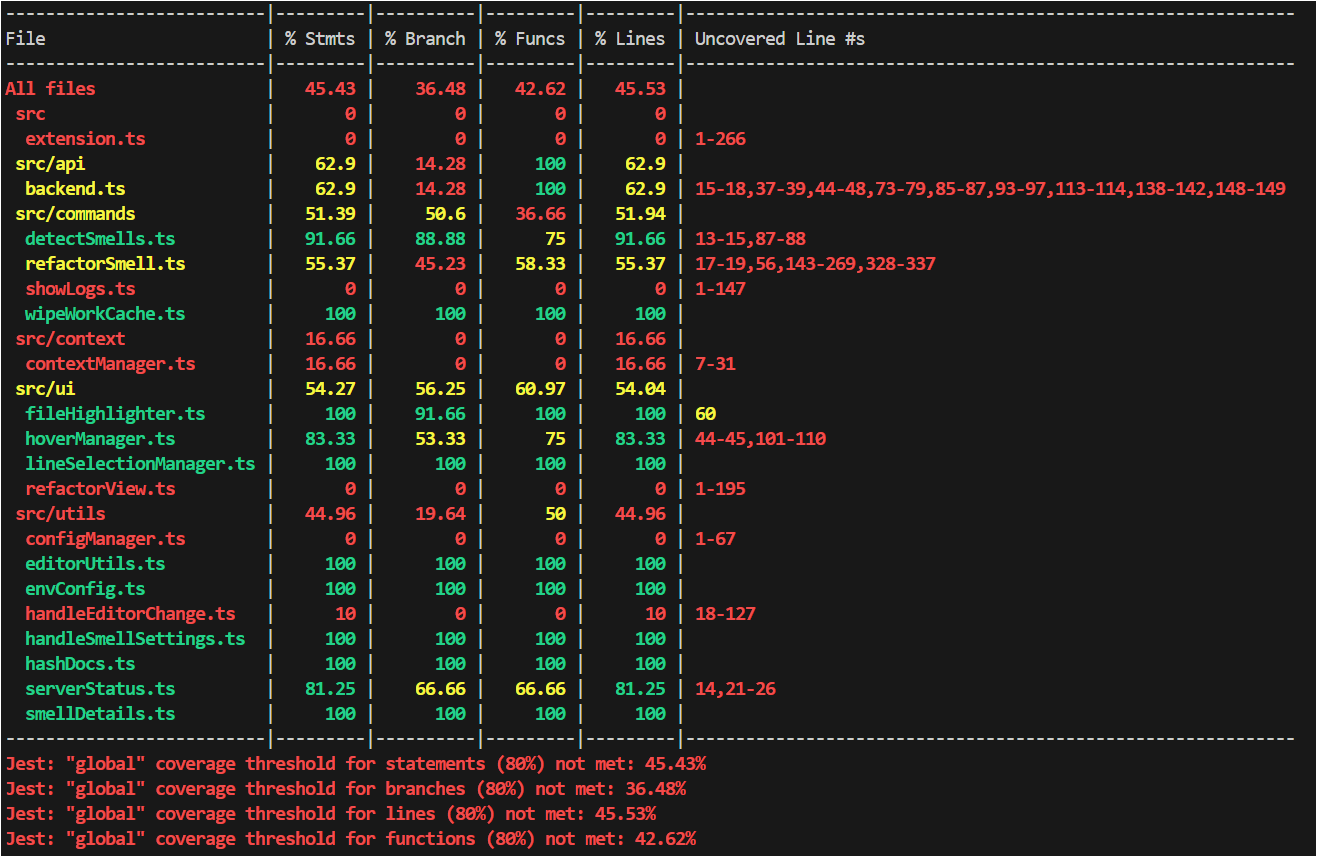
\includegraphics[width=0.7\textwidth]{../Images/vscode-coverage.png}
  \caption{Coverage Report of the VSCode Extension}
  \label{img:vscode-cov}
\end{figure}

\subsection{VSCode Extension}
The frontend codebase has an overall coverage of 96.99\% for
lines, 96.91\% for statements, 82.95\% for branches, and 95.09\% for functions
(Figure \ref{img:vscode-cov}). These metrics show significant test coverage across the codebase.

\noindent \textbf{Well-Tested Components:} Many critical components have excellent coverage, including:
\begin{itemize}
  \item \texttt{resetConfiguration.ts}: 100\% coverage across all metrics
  \item \texttt{wipeWorkCache.ts}: 100\% coverage across all metrics
  \item \texttt{hoverManager.ts}: 100\% coverage across all metrics
  \item \texttt{exportMetricsData.ts}: 100\% coverage across all metrics
  \item \texttt{trackedDiffEditors.ts}: 100\% coverage across all metrics
  \item \texttt{acceptRefactoring.ts}: 100\% line coverage (87.5\% branch coverage)
  \item \texttt{refactor.ts}: 100\% line coverage (84.61\% branch coverage)
  \item \texttt{normalizePath.ts}: 100\% coverage across all metrics
\end{itemize}

\noindent \textbf{Areas for Improvement:} The following components still require testing attention:
\begin{itemize}
  \item \texttt{backend.ts}: 98.96\% line coverage with uncovered line 124
  \item \texttt{configureWorkspace.ts}: 88.09\% line coverage with uncovered lines 59, 79-82, 91-94
  \item \texttt{detectSmells.ts}: 98.76\% line coverage with uncovered line 103
  \item \texttt{rejectRefactoring.ts}: 100\% line coverage but only 66.66\% branch coverage, with uncovered line 44
  \item \texttt{workspaceModifiedListener.ts}: 91.3\% line coverage but only 69.23\% branch coverage, with uncovered lines 58-59, 63-64, 71, 113
  \item \texttt{fileHighlighter.ts}: 95.08\% line coverage with uncovered lines 17-20
  \item \texttt{lineSelectionManager.ts}: 100\% line coverage but uncovered line 52
  \item \texttt{initializeStatusesFromCache.ts}: 97.82\% line coverage with uncovered line 96
  \item \texttt{refactorActionButtons.ts}: 87.5\% line coverage with uncovered lines 44-47, 61-64
  \item \texttt{smellsData.ts}: 100\% line coverage but only 62.5\% branch coverage, with uncovered lines 39, 117-120
\end{itemize}

\noindent \textbf{Future Testing:} While overall code coverage is excellent at 96.99\% for lines, there are still specific uncovered lines and branches in several components that should be addressed in future testing efforts. Improving branch coverage, especially in components with coverage below 70\%, should be prioritized.
\subsection{Python Backend}
The backend codebase has an overall coverage of 91\% (Figure
\ref{img:python-cov}) and has been thoroughly tested as it contains
the key features of project and the bulk of the logic. 

\noindent \textbf{Testing Exceptions:} The exception
is \texttt{show\_logs.py}, which handles the websocket endpoint for
logging, due to the complex nature of this module testing has been
omitted. Since its function is mainly to broadcast logs it is also
relatively simple to verify its functionality manually\\

\newpage
\section*{Appendix A -- Usability Testing Data} \label{appendix:usability}

\subsection*{Protocol}

\section*{Purpose}
The purpose of this usability test is to evaluate the ease of use,
efficiency, and overall user experience of the VSCode extension for
refactoring Python code to improve energy efficiency. The test will
identify usability issues that may hinder adoption by software developers.

\section*{Objective}
Evaluate the usability of the extension's \textbf{smell detection},
\textbf{refactoring process}, \textbf{customization settings}, and
\textbf{refactoring view}.

\begin{itemize}
  \item Assess how easily developers can navigate the extension interface.
  \item Measure the efficiency of the workflow when applying or
    rejecting refactorings.
  \item Identify areas of confusion or frustration.
\end{itemize}

\section*{Methodology}
\subsection*{Test Type}
Moderated usability testing.

\subsection*{Participants}
\begin{itemize}
  \item \textbf{Target Users:} Python developers who use VSCode.
  \item \textbf{Number of Participants:} 5–7.
  \item \textbf{Recruitment Criteria:}
    \begin{itemize}
      \item Experience with Python development.
      \item Familiarity with VSCode.
      \item No prior experience with this extension.
    \end{itemize}
\end{itemize}

\subsection*{Testing Environment}
\begin{itemize}
  \item \textbf{Hardware:} Provided computer.
  \item \textbf{Software:}
    \begin{itemize}
      \item VSCode (latest stable release).
      \item The VSCode extension installed.
      \item Screen recording software (optional, for post-test analysis).
      \item A sample project with \textbf{predefined code snippets}
        containing various \textbf{code smells}.
    \end{itemize}
  \item \textbf{Network Requirements:} Stable internet connection for
    remote testing.
\end{itemize}

\subsection*{Test Moderator Role}
\begin{itemize}
  \item Introduce the test and explain objectives.
  \item Observe user interactions without providing assistance unless necessary.
  \item Take notes on usability issues, pain points, and confusion.
  \item Ask follow-up questions after each task.
  \item Encourage participants to \textbf{think aloud}.
\end{itemize}

\section*{Data Collection}
\subsection*{Metrics}
\begin{itemize}
  \item \textbf{Task Success Rate:} Percentage of users who complete
    tasks without assistance.
  \item \textbf{Error Rate:} Number of errors or missteps per task.
  \item \textbf{User Satisfaction:} Post-test rating on a scale of 1–5.
\end{itemize}

\subsection*{Qualitative Data}
\begin{itemize}
  \item Observations of confusion, hesitation, or frustration.
  \item Participant comments and feedback.
  \item Follow-up questions about expectations vs. actual experience.
  \item Pre-test survey.
  \item Post-test survey.
\end{itemize}

\section*{Analysis and Reporting}
\begin{itemize}
  \item Identify common pain points and recurring issues.
  \item Categorize usability issues by severity:
    \begin{itemize}
      \item \textbf{Critical:} Blocks users from completing tasks.
      \item \textbf{Major:} Causes significant frustration but has workarounds.
      \item \textbf{Minor:} Slight inconvenience, but doesn't impact
        core functionality.
    \end{itemize}
  \item Provide recommendations for UI/UX improvements.
  \item Summarize key findings and next steps.
\end{itemize}

\section*{Next Steps}
\begin{itemize}
  \item Fix major usability issues before release.
  \item Conduct follow-up usability tests if significant changes are made.
  \item Gather further feedback from real users post-release.
\end{itemize}

\subsection*{Task List}

\section*{Mock Installation Documentation}
The extension can be installed to detect energy inefficiencies
(smells) in your code and refactor them.

\subsection*{Commands}
Open the VSCode command palette (\texttt{CTRL+SHIFT+P}):

\begin{itemize}
  \item \textbf{Detect Smells:} \texttt{Eco: Detect Smells}
  \item \textbf{Refactor Smells:} \texttt{Eco: Refactor Smell} or
    \texttt{CTRL+SHIFT+R} (or to be discovered).
\end{itemize}

\section*{Tasks}
Report your observations \textbf{aloud}!

\subsection*{Task 1: Smell Detection}
\begin{enumerate}
  \item Open the \texttt{sample.py} file.
  \item Detect the smells in the file.
  \item What do you see?
\end{enumerate}

\subsection*{Task 2: Line Selection}
\begin{enumerate}
  \item In the same \texttt{sample.py} file, select one of the
    highlighted lines.
  \item What do you see?
  \item Select another line.
\end{enumerate}

\subsection*{Task 3: Hover}
\begin{enumerate}
  \item In the same file, hover over a highlighted line.
  \item What do you see?
\end{enumerate}

\subsection*{Task 4: Initiate Refactoring (Single)}
\begin{enumerate}
  \item In the same file, refactor any smell of your choice.
  \item What do you observe immediately after?
  \item Does a sidebar pop up after some time?
\end{enumerate}

\subsection*{Task 5: Refactor Smell (Sidebar)}
\begin{enumerate}
  \item What information do you see in the sidebar?
  \item Do you understand the information communicated?
  \item Do you see what was changed in the file?
  \item Try rejecting a smell. Did the file change?
  \item Repeat Tasks 1, 4, and 5, but reject a smell. Did the file
    stay the same?
\end{enumerate}

\subsection*{Task 6: Refactor Multi-File Smell}
\begin{enumerate}
  \item Open the \texttt{main.py} file.
  \item Detect the smells in the file.
  \item Refactor any smell of your choice.
  \item Do you see anything different in the sidebar?
  \item Try clicking on the new addition to the sidebar. Notice anything?
  \item Try accepting the refactoring. Did both files change?
\end{enumerate}

\subsection*{Task 7: Change Smell Settings}
\begin{enumerate}
  \item Open the \texttt{sample.py} file.
  \item Detect the smells in the file.
  \item Take note of the smells detected.
  \item Open the settings page (\texttt{CTRL+,}).
  \item Navigate to the \textbf{Extensions} drop-down and select
    \textbf{Eco Optimizer}.
  \item Unselect one of the smells you noticed earlier.
  \item Navigate back to the \texttt{sample.py} file.
  \item Detect the smells again. Is the smell you unselected still there?
\end{enumerate}

\subsection*{Participant Data}
The following links point to the data collected from each participant:\\

{\noindent
  \href{https://github.com/ssm-lab/capstone--source-code-optimizer/blob/main/docs/Extras/UsabilityTesting/test_data/participant1-data.csv}{Participant
  1} \\[2mm]
  \href{https://github.com/ssm-lab/capstone--source-code-optimizer/blob/main/docs/Extras/UsabilityTesting/test_data/participant2-data.csv}{Participant
  2} \\[2mm]
  \href{https://github.com/ssm-lab/capstone--source-code-optimizer/blob/main/docs/Extras/UsabilityTesting/test_data/participant3-data.csv}{Participant
  3} \\[2mm]
  \href{https://github.com/ssm-lab/capstone--source-code-optimizer/blob/main/docs/Extras/UsabilityTesting/test_data/participant4-data.csv}{Participant
  4} \\[2mm]
  \href{https://github.com/ssm-lab/capstone--source-code-optimizer/blob/main/docs/Extras/UsabilityTesting/test_data/participant5-data.csv}{Participant
  5}
}

\subsection*{Pre-Test Survey Data}
The following link points to a CSV file containing the pre-survey data:\\

\noindent
\href{https://github.com/ssm-lab/capstone--source-code-optimizer/blob/main/docs/Extras/UsabilityTesting/surveys/pre-test-survey-data.csv}{Click
here to access the survey results CSV file}.

\subsection*{Post-Test Survey Data}
The following link points to a CSV file containing the post-survey data:\\

\noindent
\href{https://github.com/ssm-lab/capstone--source-code-optimizer/blob/main/docs/Extras/UsabilityTesting/surveys/post-test-survey-data.csv}{Click
here to access the survey results CSV file}.

\newpage{}
\section*{Appendix --- Reflection}

The information in this section will be used to evaluate the team members on the
graduate attribute of Reflection.

\input{../Reflection.tex}

\begin{enumerate}
  \item What went well while writing this deliverable?
  \item What pain points did you experience during this deliverable, and how
    did you resolve them?
  \item Which parts of this document stemmed from speaking to your client(s) or
    a proxy (e.g. your peers)? Which ones were not, and why?
  \item In what ways was the Verification and Validation (VnV) Plan different
    from the activities that were actually conducted for VnV?  If there were
    differences, what changes required the modification in the plan?  Why did
    these changes occur?  Would you be able to anticipate these
    changes in future
    projects?  If there weren't any differences, how was your team
    able to clearly
    predict a feasible amount of effort and the right tasks needed to build the
    evidence that demonstrates the required quality?  (It is expected that most
    teams will have had to deviate from their original VnV Plan.)
\end{enumerate}

\subsubsection*{Mya Hussain}
\begin{itemize}
  \item \textit{What went well while writing this deliverable?} \\

    One of the most rewarding parts of completing this report was
    writing and compiling
    the benchmarking and performance analysis. Seeing the data come
    to life through plots
    and visualizations was very satisfying as we could see the
    underlying patterns we
    knew existed in our code in a visual format. It also outted
    everyones performance
    on their corresponding refactorers which was cool. Overall, the
    whole process of turning raw data
    into meaningful insights was really fulfilling.  It felt like I
    was uncovering useful information that
    could really help improve the tool, which made the effort feel worthwhile

  \item \textit{What pain points did you experience during this
    deliverable, and how did you resolve them?}\\

    The biggest pain point for me was definitely the sheer amount of
    unit testing that had to
    be done before even starting the report. Writing all those tests
    and making sure everything
    worked as expected was a lot of legwork, it felt like I was stuck
    in an endless loop of running
    tests, fixing bugs, and then running more tests. It was necessary
    but not the most exciting part of
    the process. The tricky part was making sure the report actually
    reflected all that effort. As we spent hours
    testing, and finding bugs, and fixing them, so the tool is a lot
    better, but logging all of those fixes without
    1. sounding like the tool was broken to start and 2. overselling
    all the trivial tests we felt like
    we had to do to achive coverage, was a challenge.

\end{itemize}

\subsubsection*{Sevhena Walker}
\begin{itemize}
  \item \textit{What went well while writing this deliverable?} \\

    A big win was how much of our work naturally fed into the report.
    Since we had already been refining our verification and
    validation (V\&V) process throughout development, we weren't
    starting from scratch, we just had to document what we had done.
    Having clear test cases in place made it easier to describe our
    approach and results, rather than writing purely in the abstract.
    Another positive was that our understanding of the system had
    improved significantly by this point, so explaining our reasoning
    behind certain tests felt more natural.

  \item \textit{What pain points did you experience during this
    deliverable, and how did you resolve them?}\\

    One challenge was finalizing our tests while also writing about
    them. Since we were still adjusting some test cases, we had to
    ensure that any changes were reflected correctly in the report,
    which meant some back-and-forth edits. Another issue was
    balancing detail; some sections needed more explanation than
    expected, while others felt overly technical. We resolved this by
    reviewing each section with fresh eyes and making sure we
    explained things clearly without unnecessary complexity. Time was
    also a factor, as wrapping up both testing and documentation at
    the same time was a bit hectic. We managed by setting smaller
    milestones to keep things on track and making sure to check in
    regularly to avoid last-minute rushes.
\end{itemize}

\subsubsection*{Ayushi Amin}
\begin{itemize}
  \item \textit{What went well while writing this deliverable?} \\

    One of the best parts of working on this deliverable was how well
    my team collaborated. We had a clear understanding of what needed
    to be covered, which made it easier to organize our thoughts and
    avoid unnecessary back-and-forth. Writing about our unit tests
    was also pretty smooth since we had already put a lot of effort
    into designing them in the vnv-plan.
    It was satisfying to document the thought process behind them,
    especially since they played a big role in making sure the tool
    was accurate and functioned correctly.
    Another thing I really enjoyed was usability testing. It was fun
    to see how others interacted with our tool and to get real
    feedback on what worked and what did not. Seeing users struggle
    with certain parts that we thought were intuitive was interesting
    to find out, but it also made the process more rewarding because
    we could make meaningful improvements.

  \item \textit{What pain points did you experience during this
    deliverable, and how did you resolve them?}\\

    One pain point I experienced was structering the unit tests
    report and tracing back to the VnV plan tests. This is because
    The samples we had were really all over the place and not consistent at all.
    It was difficult to know what information was required for
    certian portions when most of the samples did not cover some
    portions. Also tracing back to VnV Plan tests, I realized that
    that some tests were not
    feasible and it would make no sense to do them for this project.
    Not entirely sure what we were thinking when we wrote them. So we
    decided to modify our VnV plan to be more realistic with the time
    frame we have
    and since a lot was changed in the scope of this project, we
    removed certain tests to better suit our current project.

\end{itemize}

\subsubsection*{Nivetha Kuruparan}
\begin{itemize}
  \item \textit{What went well while writing this deliverable?}

    One of the things that went well while working on this
    deliverable was our ability to catch a significant number of bugs
    and edge cases during testing. Through extensive unit and
    integration testing, we identified multiple issues related to
    multi-file refactoring, detection accuracy, and performance
    optimization. This allowed us to refine our detection and
    refactoring mechanisms, making them more reliable and robust.

  \item \textit{What pain points did you experience during this
    deliverable, and how did you resolve them?}

    One of the biggest challenges we faced was the overwhelming
    number of tests outlined in the original V\&V Plan. While
    comprehensive, implementing every test and writing detailed
    reports for each became highly time-consuming and impractical. As
    a result, we had to carefully trim down and consolidate tests to
    focus on the most critical functionalities while still
    maintaining full coverage of our system requirements. This
    process involved combining similar tests and prioritizing cases
    that had the most significant impact on correctness, usability,
    and performance. While this required careful review and
    restructuring, it ultimately streamlined the validation process
    and improved efficiency in writing the report.
\end{itemize}

\subsubsection*{Tanveer}
\begin{itemize}
  \item \textit{What went well while writing this deliverable?} \\

    The fun part was validating different requirements that we had
    defined in the VnV Plan against our tool. I saw that some of them
    were too ambitious versus others could have more points added for
    the verification. Overall, it was fun mapping non functional
    requirements against the features of the tool. At the end of it,
    I was able to deduce which NFR maps to a certain feature of the tool.

  \item \textit{What pain points did you experience during this
    deliverable, and how did you resolve them?}\\

    Writing unit tests turned out to be harder than actual
    implementation because (1) not only did I come across bugs when
    testing but also (2) mocking dependencies such as
    \texttt{vscode.workspace} for our plugin was definitely a
    learning curve. It is important to mentiont that I don't believe
    that the course and capstone would have been the same as testing,
    the team was testing left and right to get the maximum coverage.
    To resolve the learning curve I referred to multiple tutorials
    online and eventually the process became getting rid of the
    syntax errors or bugs in the unit test implementation so that the
    tests could pass.
\end{itemize}

\subsubsection*{Group}
\begin{itemize}
  \item \textit{Which parts of this document stemmed from speaking to
      your client(s) or
    a proxy (e.g. your peers)? Which ones were not, and why?} \\

    Parts of this document stemmed from speaking to users who acted
    as proxies for clients. Specifically:
    \begin{itemize}
      \item \textbf{Usability Testing Findings:} The document details
        usability testing conducted with student developers, who
        served as proxies for real-world users. Their feedback on
        sidebar visibility, refactoring speed, UI clarity, and energy
        savings feedback directly influenced the report.
      \item \textbf{Methodology and Results:} The task completion
        rates, user satisfaction scores, and qualitative insights
        were derived from these interactions, making them user-driven.
      \item \textbf{Non-functional Requirements:} This is based on
        client as some requirements like look and feel is evaluated
        by client and usability testers since they will be the ones
        using the application.
    \end{itemize}

    Parts of the document that did not stem from client or proxy
    interactions include:
    \begin{itemize}

      \item \textbf{Functional Requirements Evaluations:} These
        sections reference predefined specifications/industry
        standards rather than direct client input.
      \item \textbf{Implementation and Technical Explanations:} These
        were formulated based on the development team's decisions,
        software documentation, and prior knowledge rather than
        external feedback.

    \end{itemize}


  \item \textit{In what ways was the Verification and Validation
      (VnV) Plan different
      from the activities that were actually conducted for VnV?  If there were
      differences, what changes required the modification in the plan?  Why did
      these changes occur?  Would you be able to anticipate these
      changes in future
      projects?  If there weren't any differences, how was your team
      able to clearly
      predict a feasible amount of effort and the right tasks needed
      to build the
      evidence that demonstrates the required quality?  (It is
        expected that most
    teams will have had to deviate from their original VnV Plan.)}\\

    There were definitely some differences between what we assumed
    would happen during
    the VnV Plan and the results we actually got during testing. For
    example, the plan initially assumed that
    energy measurement times would vary significantly with file size, but the
    testing revealed that they were actually decently consistent. This meant we
    had to adjust our focus in the report to highlight the fixed
    overhead of energy
    measurement rather than exploring variability.

    For the most part, though, all of the unit testing we planned in
    the VnV Plan was
    written out per spec, and the code was fixed until all of them passed. This
    rigorous testing process actually caught a lot of bugs and edge
    cases that we
    hadn't fully anticipated in the plan. For instance, some
    refactoring operations
    worked fine on smaller files but broke on larger ones. Testing
    also revealed edge cases,
    like how the tool handled files with \textbf{multiline
    whitespace}, \textbf{nested structures},
    \textbf{degenerate/trivial input} (e.g., empty files or files
    with a single line), and
    \textbf{wrong input} (e.g., malformed code or unsupported
    syntax). These cases weren't
    explicitly called out in the original plan, but they became a big
    part of the testing process
    once we realized how critical they were to the tool's reliability.

    For example:
    \begin{itemize}
      \item \textbf{Multiline whitespace:} The tool initially
        struggled with files that had excessive or irregular
        whitespace, which caused false positives in code smell
        detection. We had to update the detection logic to handle
        these cases gracefully.
      \item \textbf{Nested structures:} Deeply nested code (e.g.,
        loops within loops or functions within functions) exposed
        performance bottlenecks and sometimes caused the tool to
        crash. This led to optimizations in the refactoring algorithms.
      \item \textbf{Degenerate/trivial input:} Empty files or files
        with minimal content revealed that some refactoring
        operations weren't properly handling edge cases, so we added
        checks to ensure the tool behaved correctly in these scenarios.
      \item \textbf{Wrong input:} Malformed or unsupported code
        caused unexpected errors, so we improved error handling and
        added clearer feedback for users.
    \end{itemize}

    Fixing these issues required additional effort, but it ultimately
    made the tool more robust and user-friendly.


    These changes happened because testing revealed patterns in the data
    and uncovered bugs that weren't obvious during the planning phase.
    The bugs and edge cases we found during testing forced us to
    revisit parts of the code and make improvements we hadn't planned
    for initially.

    Some of these changes could be anticipated in future projects
    with more thorough initial testing.
    If i could do it again I'd build more flexibility into the VnV
    Plan to account for unexpected results and allocate extra time
    for debugging and edge-case testing. I'd also include a broader
    range of test cases (e.g., multiline whitespace, wrong input) in
    the initial plan to catch these issues sooner.

\end{itemize}

\end{document}
